\documentclass[degree=master, tocarialchapter]{thuthesis}
% 选项
%   degree=[bachelor|master|doctor|postdoctor], % 必选,学位类型
%   secret,                % 可选(默认:关闭),是否有密级
%   tocarialchapter,       % 可选(默认:关闭),章目录中使用黑体(这项表示同时打开下面两项)
%   tocarialchapterentry,  % 可选(默认:关闭),单独控制章标题在目录中使用黑体
%   tocarialchapterpage,   % 可选(默认:关闭),单独控制章页码在目录中使用黑体
%   pifootnote,            % 可选(默认:关闭),页脚编号采用 pifont 字体符号,建议打开

% 所有其它可能用到的包都统一放到这里了,可以根据自己的实际添加或者删除。
\usepackage{thuthesis}
\usepackage{bm}
\usepackage{algorithm}
\usepackage{algorithmic}
\renewcommand{\algorithmicrequire}{ \textbf{Input:}}
\renewcommand{\algorithmicensure}{ \textbf{Output:}}

% 定义所有的图片文件在 figures 子目录下
\graphicspath{{figures/}}

% 可以在这里修改配置文件中的定义。导言区可以使用中文。
% \def\myname{李知赫}

\begin{document}

%%% 封面部分
\frontmatter
\thusetup{
  %******************************
  % 注意:
  %   1. 配置里面不要出现空行
  %   2. 不需要的配置信息可以删除
  %******************************
  %
  %=====
  % 秘级
  %=====
  secretlevel={秘密},
  secretyear={10},
  %
  %=========
  % 中文信息
  %=========
  ctitle={基于用户定位的广告投放服务研究},
  cdegree={工学硕士},
  cdepartment={电子工程系},
  cmajor={信息与通信工程},
  cauthor={李知赫},
  csupervisor={钟晓峰副研究员},
  % 日期自动使用当前时间,若需指定按如下方式修改:
  cdate={二〇一九年四月},
  %
  % 博士后专有部分
  cfirstdiscipline={计算机科学与技术},
  cseconddiscipline={系统结构},
  postdoctordate={2009年7月——2011年7月},
  id={编号}, % 可以留空: id={},
  udc={UDC}, % 可以留空
  catalognumber={分类号}, % 可以留空
  %
  %=========
  % 英文信息
  %=========
  etitle={Research on the Information Push Service Based on Users' Location},
  % 这块比较复杂,需要分情况讨论:
  % 1. 学术型硕士
  %    edegree:必须为Master of Arts或Master of Science(注意大小写)
  %             “哲学、文学、历史学、法学、教育学、艺术学门类,公共管理学科
  %              填写Master of Arts,其它填写Master of Science”
  %    emajor:“获得一级学科授权的学科填写一级学科名称,其它填写二级学科名称”
  % 2. 专业型硕士
  %    edegree:“填写专业学位英文名称全称”
  %    emajor:“工程硕士填写工程领域,其它专业学位不填写此项”
  % 3. 学术型博士
  %    edegree:Doctor of Philosophy(注意大小写)
  %    emajor:“获得一级学科授权的学科填写一级学科名称,其它填写二级学科名称”
  % 4. 专业型博士
  %    edegree:“填写专业学位英文名称全称”
  %    emajor:不填写此项
  edegree={Master of Science},
  emajor={Electronics Science and Technology},
  eauthor={Li Zhihe},
  esupervisor={Associate Research Professor Zhong Xiaofeng},
  % 日期自动生成,若需指定按如下方式修改:
  edate={April, 2019}
  %
  % 关键词用“英文逗号”分割
  % ckeywords={\TeX, \LaTeX, CJK, 模板, 论文},
  % ekeywords={\TeX, \LaTeX, CJK, template, thesis}
}

% 定义中英文摘要和关键字
\begin{cabstract}
  随着智能手机与移动互联网的高速发展,基于用户定位的网络服务呈现出蓬勃发展的态势。然而目前主要依赖导航卫星的定位方式只能在用户接收端定位解算且在遮挡严重的城市和室内等地方定位精度较差。与此同时,在获得用户定位后,如何有效利用这些信息也是一个研究热点。在这些应用中,有一类广告投放问题,依据用户位置筛选出广告投放的候选用户群,在保证投放量的同时尽可能得到最优的广告投放效果。为了解决上述问题,我们提出了一种基于用户定位的广告投放服务机制,它只需要接收信号强度就可以实现用户定位,并且在后续的广告投放中可以获得更好的广告投放效果。在本文中,我们先提出了两种用户定位方法,分别是以用户作为信号发射源的定位解算算法和以用户作为信号接收端的指纹定位算法,二者相比于各自方向的经典算法均能提高定位精准度。在获得用户位置之后,我们提出一种基于凸优化的保量推荐下的最优广告投放算法,在提高广告投放效果的同时还有较低的在线计算复杂度。

  本文的主要贡献如下:
  \begin{itemize}
    \item 提出一种新的定位算法实现对发射源定位,并分析其克拉美罗下界(Cram\'{e}r-Rao Lower Bound)和置信区间。仿真实验显示,当噪声较大时我们的新算法可以取得比经典的最大似然算法更小的误差,而实测数据实验结果表明新算法相比于最大似然法可以在均方根误差和平均绝对值误差上分别减少18.9\%和25.7\%;
    \item 将切线距离引入指纹定位的距离度量方法,并提出曼哈顿切线距离的计算方法及其近似算法。在校园内实地采集的接收信号强度数据上开展的实验表明,曼哈顿切线距离及其近似算法相比于曼哈顿距离分别在均方根误差上平均降低了7.45\%和5.02\%;
    \item 给出一种保量推荐下的最优广告投放算法,基于凸优化原理推导出广告投放方案,并介绍一些工程实现细节增强算法的稳健性和适用性。仿真实验证实了该算法相比于简单贪心算法可以在点击率上相对提升29.0\%。此后该算法被部署在快手短视频平台上,持续一个月的线上实验表明,对于关键指标——关注率,该算法相比于之前部署的算法相对提高了3.48\%,而在其他次要指标上持平或略有提升,且算法性能可以经受住大流量的考验。
  \end{itemize}


\end{cabstract}

% 如果习惯关键字跟在摘要文字后面,可以用直接命令来设置,如下:
\ckeywords{定位, 保量推荐, 最优投放,优化算法, 接收信号强度}

\begin{eabstract}
   With the rapid development of smartphones and mobile Internet, the network service based on users' location is developing vigorously. However, the current mainly applied localization technology is based on satellite signal, which suffers from some limitation. For example, the location can only be computed at users' clients and satellite signal is vulnerable to shelter, which is common in cities and indoor situation. Meanwhile, under the condition of users' location being available, the methods to efficiently employ these information has drawn increasing attention. Among these methods, there is a kind of advertising problem, where we will select candidate user group according to users' location and then we aim at optimizing the allocation effect of advertisement (ad) with advertisers' delivery quantity guaranteed. In order to solve the above problems, we propose an ad allocation service mechanism based on users' location, where the localization only needs the received signal strength and the following ad allocation effect is better than the previous algorithm. In this thesis, we firstly propose two user localization algorithms with respect to taking users as signal transmitters and \textit{Fingerprint Localization}, where users are taken as receivers. These two algorithms both outperform the classical algorithms in each field. After users' location is available, we propose an optimal ad allocation algorithm based on convex optimiaztion with allocation quantity guaranteed, which can improve the allocation effect with low online computational complexity. 
   
   The main contributions of this article are as follows:
   \begin{itemize}
   	\item We propose a novel localization algorithm to localize transmitters. The Cram\'{e}r-Rao Lower Bound and confidence interval are analyzed. Simulation results demonstrate that our algorithm can achieve less localization error compared with classical Maximum Likelihood algorithm when noise increases. Experiments based on measured data verify that our algorithm can achieve 18.9 \% less Root Mean Square Error (RMSE) and 25.7\% less Mean Absolute Error (MAE) compared with Maximum Likelihood algorithm.
   	\item We introduce the tangent distance to the distance metrics of Fingerprint localization. Meanwhile, the computational method of Manhattan tangent distance and its approximate computational method are proposed. Experiments are carried out based on the received signal strength data collected on campus, which verify that the RMSE of localization can be decreased in 7.45\% and 5.02\% with respect to Manhattan tangent distance and its approximate one compared with simple Manhattan distance.
   	\item We propose an optimal ad allocation algorithm with allocation quantity guaranteed. Allocation strategy is derived with convex optimization theory and some engineering implementation details are also described to make the algorithm more robust and generalized. Simulation result reveals that the Click-Through Rate of our algorithm is 29.0\% more than the simple greedy algorithms. Afterwards, the algorithm is deployed at Kwai video platform for a month. The result of the online experiment demonstrates that our algorithm achieves 3.48\% more than the previously deployed algorithm on the  key metric, which is Follow Rate, and performs equally on the other secondary metrics. Furthermore, it is stable under huge network traffic. 
   \end{itemize}
   
\end{eabstract}

\ekeywords{localization, guaranteed delivery advertising, optimal allocation, optimization algorithm, received signal strength}

% 如果使用授权说明扫描页,将可选参数中指定为扫描得到的 PDF 文件名,例如:
% \makecover[scan-auth.pdf]
\makecover

%% 目录
\tableofcontents

%% 符号对照表
\begin{denotation}[3cm]
\item[WAP] 无线网络接入点 (Wireless Access Point)
\item[RSS] 接收信号强度(Received Signal Strength)
\item[ML] 最大似然(Maximum Likelihood)
\item[GBM] 基于几何的模型(Geometry-Based Model)
\item[KNN] K近邻(K-Nearest Neighbors)
\item[ETD] 欧式切线距离(Euclidean Tangent Distance)
\item[MTD] 曼哈顿切线距离(Manhattan Tangent Distance)
\item[AMTD] 近似曼哈顿切线距离(Approximate Manhattan Tangent Distance)
\item[PIKA] 最优快手广告投放算法(oPtImal Kwai Advertising)
\item[FC] 流量控制算法(Flow Control)
\item[LP] 线性规划(Linear Programming)
\item[CTR] 点击率(Click-Through Rate)
\item[FTR] 关注率(Follow Rate)
\item[PV] 页面访问(Page View)
\end{denotation}



%%% 正文部分
\mainmatter
\chapter{引言}
\label{cha:intro}

\section{研究背景}
近年来,随着智能手机的普及以及移动互联网的快速发展,基于移动互联网以及用户位置的应用正呈现井喷式的增长,而因为LTE网络的普及以及5G的即将到来,智能终端将与日俱增,与之对应的高精度定位也将变得更加重要,比如自动驾驶中的高精度定位。除此之外,定位技术还广泛应用于商业广告、购物消费、医疗保健、险情救援等诸多领域,从传统的手机定位导航到近几年兴起的网约车以及共享单车都是用户定位改变人们生活的典型范例。正因为定位是众多应用的基础必需模块,定位问题及其后续服务一直是学术界的研究热点。

\subsection{定位问题}

在开阔的室外环境中,以 GPS(Global  Positioning System)和北斗为代表的卫星定位系统已经能够实现准确的定位~\cite{xiao2016survey},这也是目前定位算法最成功的的实现之一。然而,卫星定位仍然存在一些目前无法妥善解决的问题。首先,卫星定位的结果只能在终端(client)解算得到,因此服务端(server)只能依靠用户上传自己的位置从而得知其位置。这在某些场景下是不适用的,比如对非法电台的定位。其次,卫星定位需要用户终端硬件支持卫星信号,这不仅增加手机制造的成本,而且对于不支持卫星定位的老旧手机无法定位。最后,由于卫星信号强度弱使得其抗干扰和遮挡能力弱,因此卫星定位在室内和高楼遮挡较多的市区无法准确定位。

目前基于非卫星信号的定位主要应用于室内定位(Indoor Localization)和无线传感器网络(Wireless Sensor Network)定位。在这些场景下,多种特征可以被用于定位,包括接收信号强度(Received Signal Strength, RSS)~\cite{vaghefi2013cooperative, jackson2011received, liu2006analysis, bahl2000radar}、信号到达时间(time-of-arrival)~\cite{guvenc2009survey}、到达时间差(time-difference-of-arrival)~\cite{catovic2004cramer}和到达角(angle-of-arrival)~\cite{cong2002hybrid}。其中,到达时间需要终端和无线接入点(Wireless Access Point, WAP)时间同;,到达时间差一般是无线电信号和另一个慢速传播信号(比如超声波)的传播时间差,因此需要额外设备;到达角需要天线阵列从而提高了该方法的成本和能耗。只有基于RSS的方法不需要额外的硬件因为信号强度是实现通信的最基本要求。此外,美国国家通讯委员会于2005年提出了E911紧急定位要求:定位精度在67\%的概率下处于50m \textasciitilde 100m区间,以95\%的概率处于150m \textasciitilde 300m区间~\cite{junglas2008location}。只有基于RSS的定位算法可以在当前条件下实现对所有手机的定位。因此我们的研究将专注于基于RSS的定位算法。

\subsection{广告投放问题}

在解决定位问题获得用户位置后,如何更好的使用也是一个有意义的课题。其中,基于用户定位的广告投放吸引了越来越多的关注。“2016年网络广告市场规模已达2902.7亿元, 其中移动网络广告超过60\%”~\cite{赵杨2018基于机器学习混合算法的},将用户位置信息应用于移动网络广告使得广告投放更精准是一个重要的课题。保量推荐广告(Guaranteed Delivery Advertisement)是互联网企业的主要收入来源之一~\cite{korula2016optimizing, mcafee2013maximally},广告主事先设定广告投放量和投放时长,广告平台则是在确保广告获得足够曝光量的前提下,取得尽量好的投放效果(比如点击率,关注率等)。针对这个问题,文本将提出一种基于用户定位的最优保量推荐算法。

我们将每次用户刷新页面称作一次页面访问(Page  View, PV)。在经过上游服务的处理后,到达广告服务器的每次PV都会携带候选投放广告以及预测出的该用户对于这些广告的打分,我们将在候选广告中选取一个或几个广告投放给该用户或者均不投放。在PV流中选择用户投放广告来最大化总的分数且保证曝光量并不是一件显而易见的事,因为决定投放哪条广告必须在几百毫秒量级的时间内决定,因此不可能将所有访问请求累积起来然后从中选几个最优的投放。一种最简单的实现则是针对每次访问,选择分数最高的广告,若分数最高的广告投放量已满则选择次高,以此类推。但是因为贪心法的如下缺点,现实中这种实现方式并不适用:
\begin{itemize}
	\item 高质量广告即几乎所有用户对其打分都高的广告会快速投放完毕而低质量广告甚至可能无法保证曝光量。因为平稳投放也是我们的一个次要目标,所以该方法不适用;
	\item 该方案的投放结果与最优结果相去甚远。例如表\ref{tab:eoa}所示,有3次访问和2个广告,每个广告的投放量都是1。显然,最优投放策略应该是广告1 $\rightarrow$ PV 1,广告2 $\rightarrow$ PV 3,该策略总分是1.2。然而上文的贪心法策略是广告1 $\rightarrow$ PV 2,广告2 $\rightarrow$ PV 1,总分只有0.7。
\end{itemize}
\begin{table}[b]
	\centering
	\caption{广告投放举例}
	\label{tab:eoa}
	\begin{tabular}{ccc}
		\toprule
		分数 & 广告 $1$ & 广告 $2$ \\
		\midrule
		PV $1$ & $0.5$ & $0.6$ \\
		\midrule
		PV $2$ & $0.1$ & $0.2$ \\
		\midrule
		PV $3$ & $0.3$ & $0.7$ \\
		\bottomrule
	\end{tabular}
\end{table}
为了解决上述问题,我们提出了一种保量推荐下的最优广告投放算法。

为了验证算法的性能与效果,我们将算法部署到了快手的广告平台上。快手(Kwai)作为世界上最大的短视频平台之一,为视频作者提供名为“粉丝头条”的服务来帮助他们推广自己的作品,本质上是一种保量推荐广告。粉丝头条的购买者需设定期望的曝光量(即该视频出现在他人视频页面上的总次数)和投放时长,我们在确保曝光量的同时使得投放结束后购买者获得最多的粉丝数(即关注量或订阅量)增加。快手的视频页面分为“关注”、“发现”和“同城”三栏,如图\ref{fig:kwai}所示,广告将以图中一个视频栏的形式出现。同城页的视频按照访问者与视频作者之间的距离筛选,我们的算法将部署在快手同城页粉丝头条服务中。

\begin{figure}[tb]
	\centering
	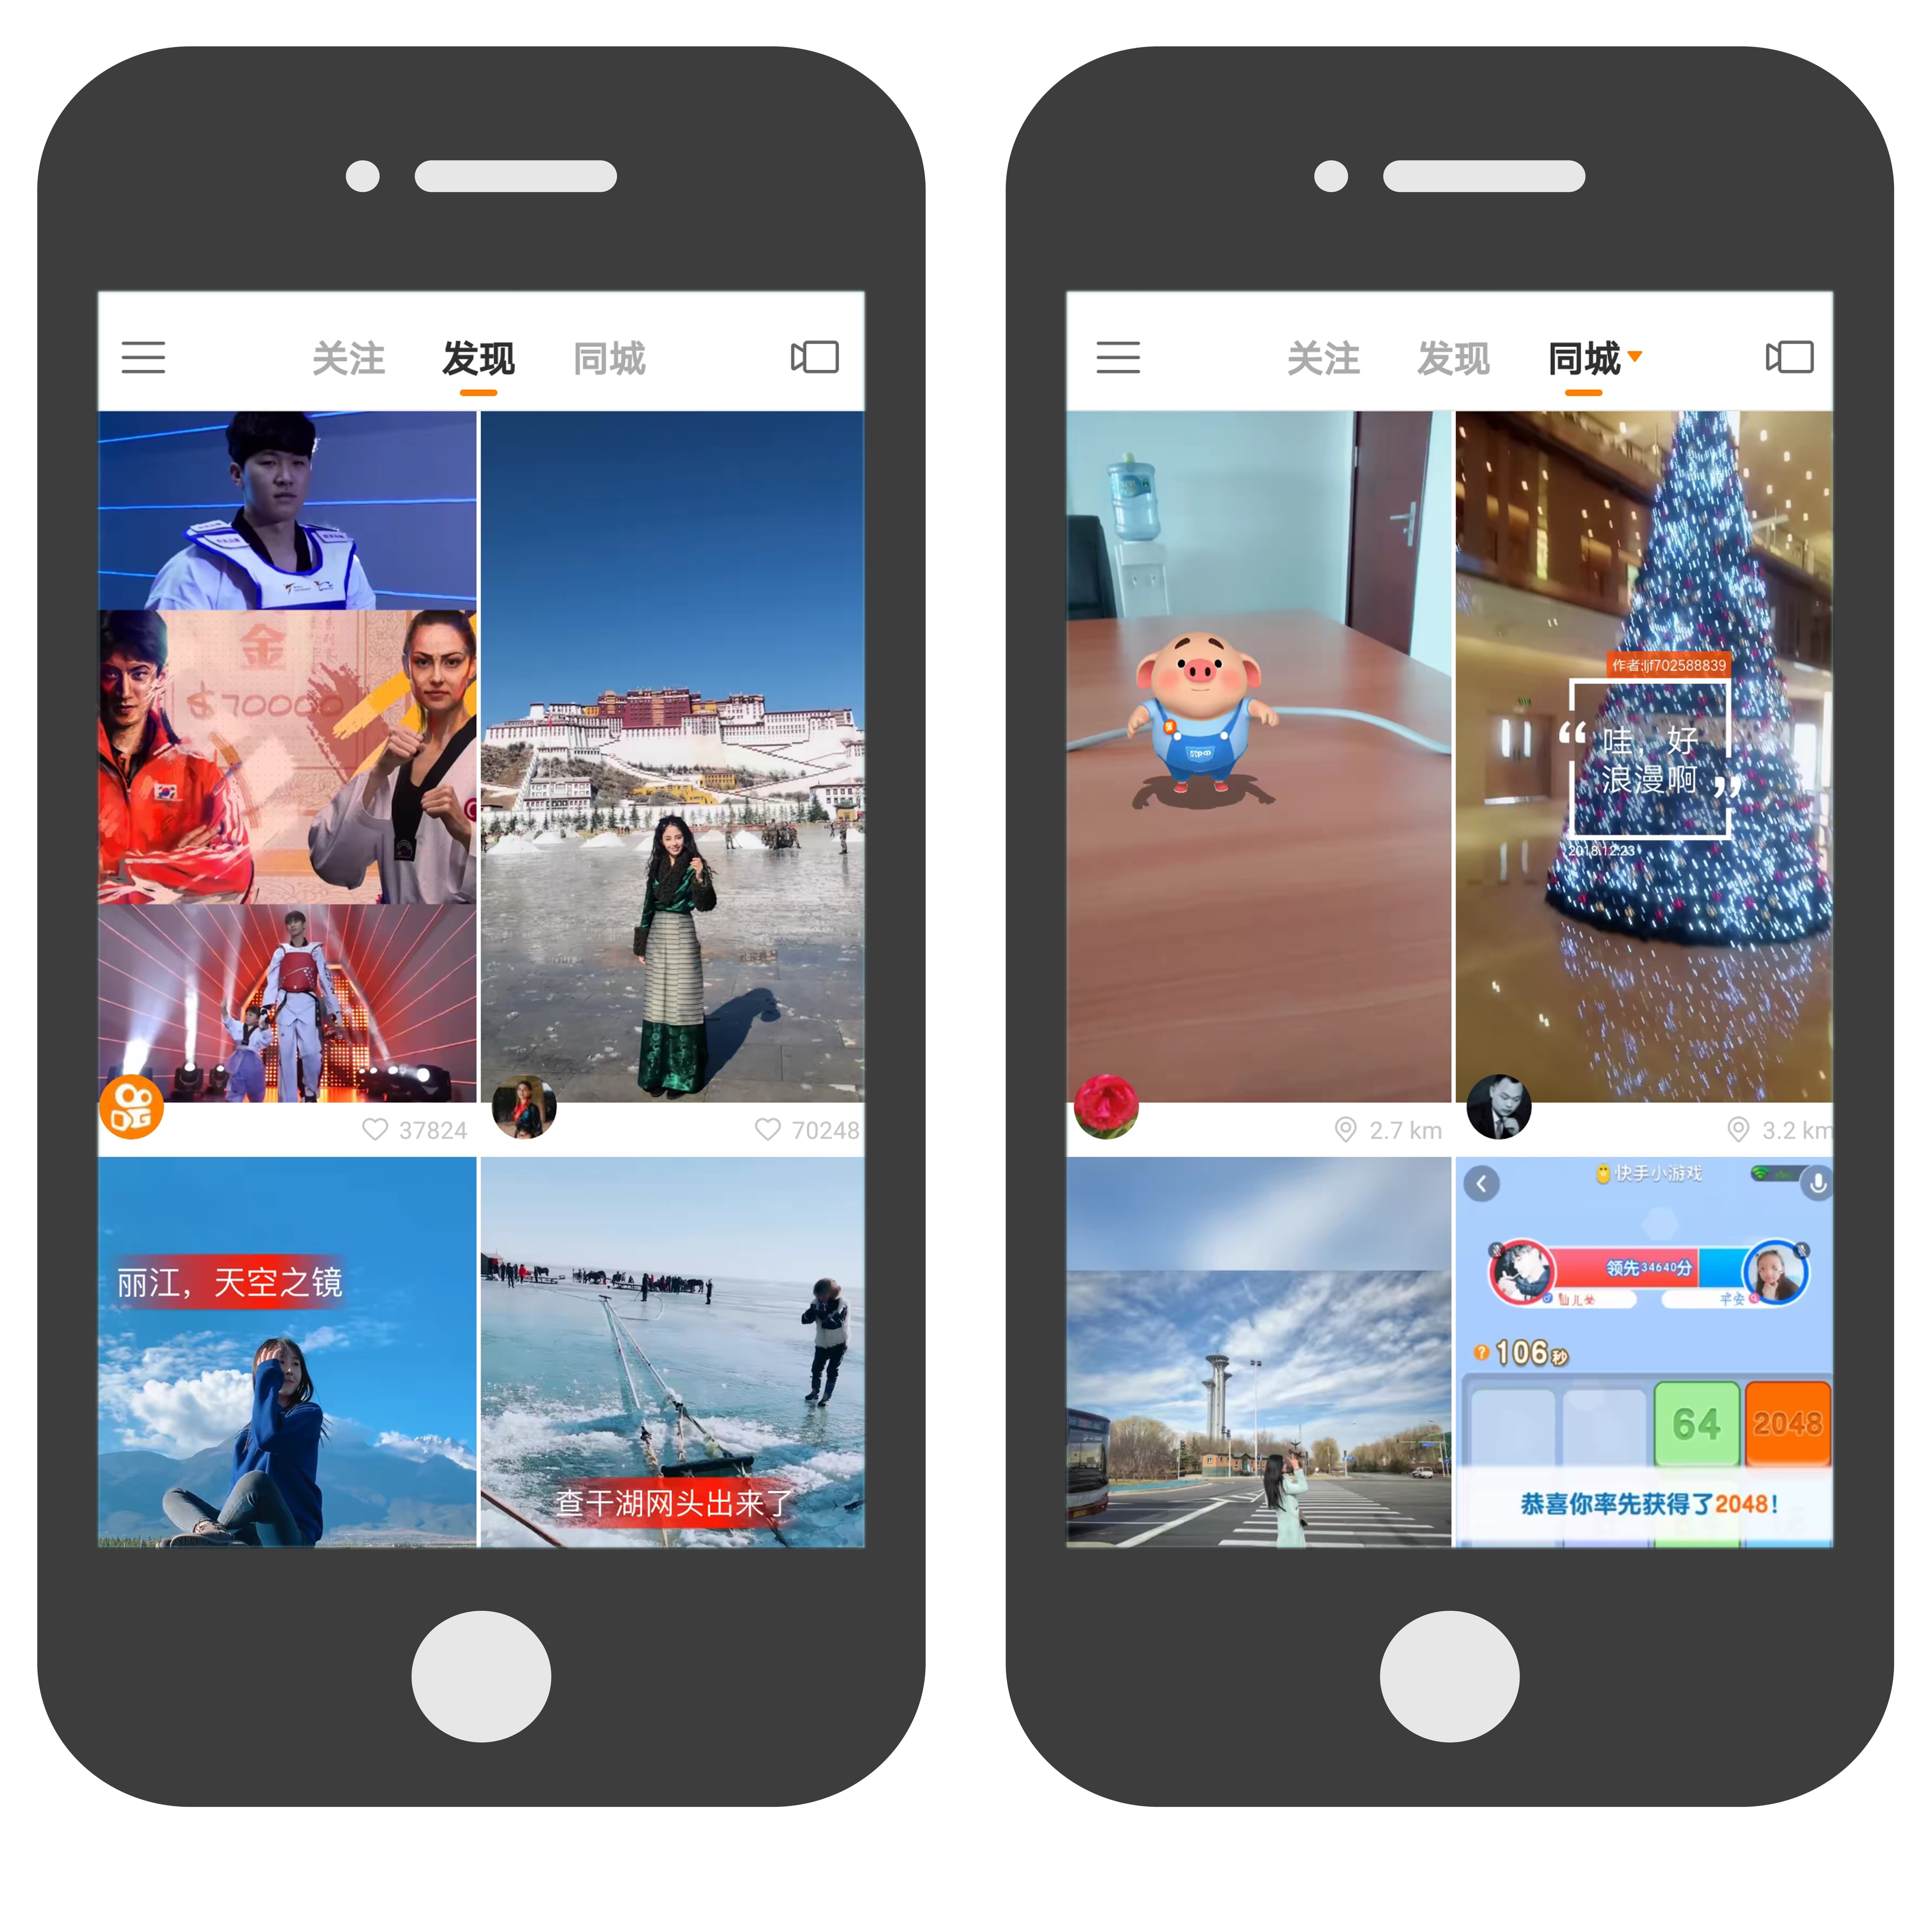
\includegraphics[width=0.75\textwidth]{Kwai.jpg}
	\caption{如图所示为快手发现页和同城页的页面设计,本文主要关注右子图即同城页。在同城页展现给用户的视频会先根据用户与视频作者之间的距离筛选。}
	\label{fig:kwai}
\end{figure}

\section{定位与广告投放算法的研究现状}
\label{sec:first}

\subsection{定位方法的研究现状}

上一小节中我们根据定位所采用的信号特征将定位算法分类,其中只有基于RSS的方法不需要额外硬件且兼容现有通信设备,因此这里仅分析研究基于RSS的定位算法。

我们可以按照定位目标是信号发射源还是接收端来对算法分类。当用户作为信号发射源时,他的位置是由分散在其周围的信号接收节点根据RSS联合计算获得的。因此该方法所得的位置信息是在服务端解算获得的,若用户想获知自己的位置需要向服务器请求。与之对应的,当用户作为信号接收端时,通过在终端汇总定位信号并在本地解算或者上传到服务器解算获得其位置。举例来说,非法电台定位场景下的算法就是前者,而卫星定位是后者的典型代表。

此外,在基于RSS的定位中,如果按照定位算法的求解方式分类,还可以将算法分为基于求解优化问题或是基于模式识别。前者需要对信号传输模型建模,设计误差函数后求解定位位置使其最小。后者需要大量采集当地信号作为指纹(Fingerprint)或者数据库(Database),在定位时设计算法将当前信号与指纹/数据库进行匹配得到位置,这种方法又被称为“指纹定位”(Fingerprint Localization)或“数据库相关算法”。前者不需要大量的事先数据采集工作且泛化能力强,但是信道建模是一个难点,因为简单模型不能反应真实情况从而降低定位准确性,而复杂模型又会提高计算复杂度。同时,前者一般都是非凸优化问题从而导致求解困难。反之,后者不需要复杂的建模工作而且一般来说定位精度更高,不过需要大量的数据采集而且一旦在一个新的区域定位就必须重新采集数据。发射源定位多采用前者因为不同用户作为发射源时其发射功率无法保证相同,而且一旦用户移动,所有位置的RSS都会变化。接收端定位则二者兼有实现实例,但在室内定位中多采用指纹定位,因为后者定位精度高且定位区域小,数据采集简单。

接下来我们将分别从基于求解优化问题的定位和指纹定位两个方面综述。

\subsubsection{基于求解优化问题的定位}

使用该方法定位有一个最基本假设即发射源功率是恒定的,一般来说这个假设都可以满足。该方法可以被分为两类:有锚点(Anchor Point)和无锚点,其中锚点是一个到发射源距离已知的点。在无线传感器网络中锚点很常见,但是在某些场景下这个假设过强,比如定位非法电台。在后续讨论中我们只关心无锚点的情况。

在无锚点的情况下,最大似然法(Maximum Likelihood, ML)是最常用的估计器和基准(Baseline)。许多其他基于ML的估计器被提出了,但是无论是半正定规划(Semidefinite Programming)还是线性最小二乘(Linear Least Square, LLS)都不能取得比ML更低的误差~\cite{jackson2011received}。这些估计器的改进点在于将原来的非凸优化问题转化为凸优化问题,虽然改变后可以保证取得最优解从而提高了求解效率,但是改变目标函数也使得新问题的最优解依然不是原问题的最优解,因此会在不同程度上降低定位精度。

S. Wang 和 R. Inkol~\cite{wang2011near}提出了两种基于LLS的算法,其推导过程表明每两个信号接收点可以形成一个发射源坐落在其上的圆。但是,作者之后提出了两种LLS解法而没有再针对这个现象深入研究。我们将提出一种算法,利用这些圆的几何意义实现发射源定位,即找到一个点使得它到所有圆边缘的距离之和最小。一种利用类似方式来实现发射源定位的算法已经被提出~\cite{liu2006analysis},但是这篇文章的应用场景是有锚点的。

\textit{克拉美罗下界(Cram\'{e}r-Rao Lower Bound, CRLB)}是估计器对于一个确定但未知的值进行估计时,估计器方差的下界。对其进行理论分析和研究有利于了解估计器的最优性能,减小数据噪声对估计器性能评估的影响。

\textit{置信区间(Confidence Interval)}是对于某一未知参数,以区间形式给出其可能的估计值。因为噪声的影响,均值的不同并不能说明两个估计量统计显著的不同,而置信区间提供了一个简便的判断方法。如果两个均值均不在对方的双边$1-\alpha$置信区间内,则二者以显著水平为$\alpha$不同。我们可以据此判断两个算法所得的定位误差的差距是否具有统计显著性。

\subsubsection{指纹定位}

如本节开篇所述,指纹定位是对基于模式识别的定位算法的别称。指纹定位能够比传统算法表现更好是因为后者需要视线内通信~\cite{gentile2012geolocation},而这个条件对于城市内和室内定位来说过于严苛。指纹定位由线下建库和线上定位两部分组成。在线下建库部分,需要根据物理空间中的不同地点的坐标和信号空间中对应的RSS构建对应关系,并形成数据库。线上定位部分则根据输入的RSS在数据库中进行匹配,之后根据不同的算法实现定位。

指纹定位有多种实现方式,从K近邻(K Nearest Neighbors, KNN)到支持向量机(Support Vector Machine, SVM)和深度学习(Deep Learning, DL)。因为其计算成本低且定位效果好,KNN及其衍生算法在指纹定位中被广泛使用~\cite{xia2017indoor}。加权KNN(Weighted-KNN)是KNN的诸多衍生算法中的一个,它的定位精度优于经典KNN~\cite{yen2017modified}。

除了代表近邻数的参数$k$,距离度量方式也是KNN中的一个重要参数。一些常用的度量方式经常被采用并比较定位效果,比如欧氏距离(Euclidean Distance)、曼哈顿距离(Manhattan Distance)和余弦相似度(Cosine Similarity)。目前已经有一些文章针对这些常用度量方式的定位效果进行比较。当曼哈顿距离与欧氏距离和谷本距离(Tanimoto Distance)比较时,曼哈顿距离定位精度更高~\cite{marques2012combining}。在某些情况下,余弦相似度也会取得比欧氏距离更小的误差~\cite{han2015cosine}。上述所有度量方式都给予大RSS和小RSS相同的权重,但这可能并不是一种理想的选择。指数变换法被提出来解决这个问题~\cite{torres2015comprehensive},但是变换中参数对结果的影响没有被分析,相关的实验会在本文中开展。

切线距离(Tangent Distance)最早被提出以解决手写数字识别问题~\cite{simard1998transformation},它是对于流形(Manifold)之间距离的局部线性近似。流形是机器学习领域中的经典假设,即高维输入数据一般都居于或邻近低维流形~\cite{roweis2000nonlinear},并且数据的微小扰动会形成流形。在这种情况下,两点之间的真实距离并不是简单的二者之间的距离而是这两个点所在的不同流形之间的距离。在原文中,切线距离是基于欧氏距离的,不过在我们的实验中欧氏距离定位精度并不如曼哈顿距离。因此我们将提出一种基于曼哈顿距离的切线距离来提高定位精度。

\subsection{广告推送算法的研究现状}

预算广告(Budget Advertising)在过去几年正在吸引越来越多的关注。快手的粉丝头条广告和目标广告(Target Advertising)~\cite{xu2015smart}以及搜索广告(Search Advertising)~\cite{mehta2005adwords}有很多相似之处。广告主在目标广告中设定一些目标用户的属性,而在搜索广告中设定一些在线搜索关键字。我们的场景与二者的不同之处在于我们的约束是实际曝光量最好等于期望曝光量,而后两者的约束是广告消费金额不能超过广告主的预算,即我们是等式约束,而后两者是不等式约束。同时,几乎所有的目标广告和搜索广告的目标都是最大化收入或者平稳投放,而我们的目标是最大化投放效果。因此这些算法需要相应的修改以适应我们的问题。Feldman et al. ~\cite{feldman2010online}证明了基于训练的对偶法(primal-dual)的有效性,但是因为文中的目标函数是线性函数,导致在线投放机制是启发式的。Devanur 和 Hayes~\cite{devanur2009adwords} 提出了一种平滑的线性规划(Linear Programming, LP)来避免竞价时出现相同竞价权重的问题。但是,该方法目标是最大化收入,而我们的目标是最大化点击率(Click-Through Rate, CTR)或者关注率(Follow Rate, FTR)。此外,他们的约束是广告平台从广告主的收费不能超过广告主的预算,不同于我们的实际曝光量最好和期望曝光量相等。针对我们的问题的解决,类似的公式曾被 Turner 提出过~\cite{turner2012planning},他的目标函数是二次函数且是等式约束。但是求解过程引入了除法操作,这在我们的算法实践中可能会造成严重问题,因为用户对视频的打分在 $10^{-5}$ 到 $10^{-2}$ 范围内变化,所以分数上的微小变化将会引起倒数的剧烈变化,即该解法使得问题病态。最后,实时竞价广告(Real-Time Bidding Advertising)和预算广告也有很多相似之处,Chen et al.~\cite{chen2011real} 提出了一种类似的基于LP的算法。

此外,一些研究分析了LP算法的解对最优解的逼近程度。Devanur et al.~\cite{devanur2011near} 证明了在独立同分布的情况下,算法结果和最优解之比为 $1-O(\epsilon)$,其中 $\epsilon$ 是一个常数。深入的研究证明即使分布随时间变化,这个比例仍然能够达到 $1-\frac{1}{\sqrt{k+3}}$,其中 $k$ 代表最小容量~\cite{alaei2012online}。

我们的算法要部署在快手的商业化平台上,而快手的日均访问量是百亿级别的,因此除了广告投放效果之外,算法的计算时间和响应时间也是至关重要的。为了实现从理论到实践的过渡,有三大类实现方式:贪心法,启发式算法和凸优化。
\begin{itemize}
	\item Karande et al.~\cite{karande2013optimizing} 提供了一种快速贪心算法并且他们也把优化CTR纳入了考虑范围。但是贪心法的问题是没有考虑到广告之间的互相影响。比如某次访问对广告1来说虽然分数比广告2高,但是广告1自身看来并不是高分,却可能在广告2看来已经是高分了。那么贪心地把广告1分配给该次访问就会降低总分数;
	\item Agarwal et al.~\cite{agarwal2014budget}提出了预算调整算法(Budget Pacing Algorithm),这也是之前在快手粉丝头条平台部署的算法,又叫做“流量控制”或“流控”(Flow Control, FC)。算法原理是根据历史数据针对每个广告设置分数阈值,并且周期性的调整。对于每次访问中的候选广告,通过阈值的广告将加入最高分数竞价,即选出分数最高的广告。这个算法原理简单、容易实现,并且在快手表现良好,不过仍然有一些问题:
	\begin{itemize}[*]
		\item 这是一个次优的启发式算法。算法过程相当于把不可能是最优解的情况排除掉,但是从某种程度上依然会出现和贪心法同样的问题;
		\item 阈值不易设置,大量的精力需要投入其中以得到稳定的投放效果。
	\end{itemize}
	虽然如此,但是流控只需要少量的计算并且只依赖于分数的偏序关系而不是绝对数值,这使得它抗噪能力更强。流控在本文后续的实验中是作为A/B测试的基准;
	\item 基于凸优化的算法有许多变种。SHALE~\cite{bharadwaj2012shale} 和 Vee et al.~\cite{Vee2010Optimal} 的方法启发了我们用 KKT 条件和坐标下降的方法解凸优化问题。但是,仅仅依靠概率是不够保证曝光量尽量接近广告主的期望量的。Agrawal et al.~\cite{agrawal2014dynamic} 求解了一个LP问题,其中对偶法中的对偶变量变成了出价阈值,决定着是否投放该广告。然而该算法没有约束每次访问最多投放广告数量,从而导致较难扩展以适应我们的需求。Huang et al.~\cite{huang2016online} 通过屏障(Barrier)函数将约束优化问题转化为无约束优化问题,但是在线计算梯度下降法可能会严重影响响应时间。Kesselheim et al.~\cite{kesselheim2014primal} 通过按比例求解部分已知的原问题并且随机地多次循环求解,最终针对每次访问得到全部的投放策略,而且文中还分析了最优逼近率。但是和上一个方法一样,在线求解LP问题可能会使得用户等待时间过长。
\end{itemize}

最后,每天的访问流量并不是平稳的,因此 Lee et al.~\cite{lee2013real} 针对每天中不同的时间段分配不同的预算权重。这种方法和我们采用的“小时需求量”策略不谋而合。

从上文可以发现,因为我们的目标是最大化广告分数,所以需要事先知道用户对广告的打分,而在我们的情况下分数就是CTR和FTR的线性组合,因此CTR和FTR的预测也是广告投放中的重要组成部分。但是限于篇幅原因,这些不会在本文中被详细介绍。如果您感兴趣,Chapelle et al.~\cite{chapelle2015simple} 描述了CTR和转化率预测的细节。

\section{论文主要研究内容及组织结构}

本文提出了一种基于用户定位的广告投放服务机制,并介绍其系统架构。文章由定位和广告投放两大部分组成。在定位部分,分别基于用户是信号发射源或接收端的场景,提出基于几何模型的定位算法和基于曼哈顿切线距离的指纹定位算法,仿真实验和实测数据验证了新算法均优于基准算法的定位精度。广告投放部分,提出一种保量推荐下的最优广告投放算法,利用凸优化中的对偶法求解广告投放策略,同时介绍一些工程实现上的细节,最后仿真实验和持续一个月的线上实验验证了算法性能与效果。

论文后续章节如下组织:

第\ref{cha:sys_arch}章介绍基于用户定位的广告投放服务的总体系统架构,之后重点介绍广告投放系统的架构。

第\ref{cha:transmitter}章在用户作为信号发射源时对用户定位。首先介绍基于RSS的几何模型定位算法原理,理论推导与蒙特卡洛法(Monte Carlo)相结合给出新算法的CRLB。为了确认定位精度的提升具有统计显著性,后续给出均方根误差(Root Mean Square Error, RMSE)的置信区间的推导方法。最后介绍仿真场景设置以及真实路测数据的采集情况,分析实验结果。

第\ref{cha:fingerprint}章在用户作为信号接收端时对用户定位。首先介绍指纹定位中常用的几种距离度量方式并分析其存在的缺陷,从而引出指数变换法和切线距离。之后按照 Simard et al.~\cite{simard1998transformation} 的定义介绍基于欧氏距离的切线距离,进而提出基于曼哈顿距离的切线距离。我们分别提出了曼哈顿切线距离的相对精确解法和近似解法,并分析其计算复杂度。最后介绍实验数据采集情况,分析上述方法在实验中的表现。

第\ref{cha:allocation}章介绍保量推荐下的最优广告投放算法。首先给出问题的数学定义,利用KKT条件求解对偶变量,进而得到广告投放策略。其后,介绍几个该算法在工程实现中的细节,使得算法能够真正部署到大流量的广告平台上。通过设置简单的仿真实验,前期验证算法相比于简单贪心法可以获得投放效果的提升后,我们开展为期一个月的线上实验,测试并分析算法的性能以及效果。

第\ref{cha:conclusion}章总结本文主要研究内容,并根据目前的内容展望进一步工作。



\chapter{基于用户定位的广告投放服务系统架构}
\label{cha:sys_arch}

因为我们的系统同时涵盖了用户定位和广告投放的功能,因此只要是需要定位以实现精准广告投放的场景都适用于这套系统。比如,本文所实现的场景是根据用户和广告主之间的定位,在快手短视频平台上给用户投放广告。除此之外,基于室内定位技术,在购物中心内将附近的商家广告推送给顾客也是一种可能的应用场景。

本章将要介绍基于用户定位的广告投放服务系统的总体结构,之后详细阐述定位和广告投放两个模块的系统架构。

\section{总体系统结构}

\begin{figure}[htb]
	\centering
	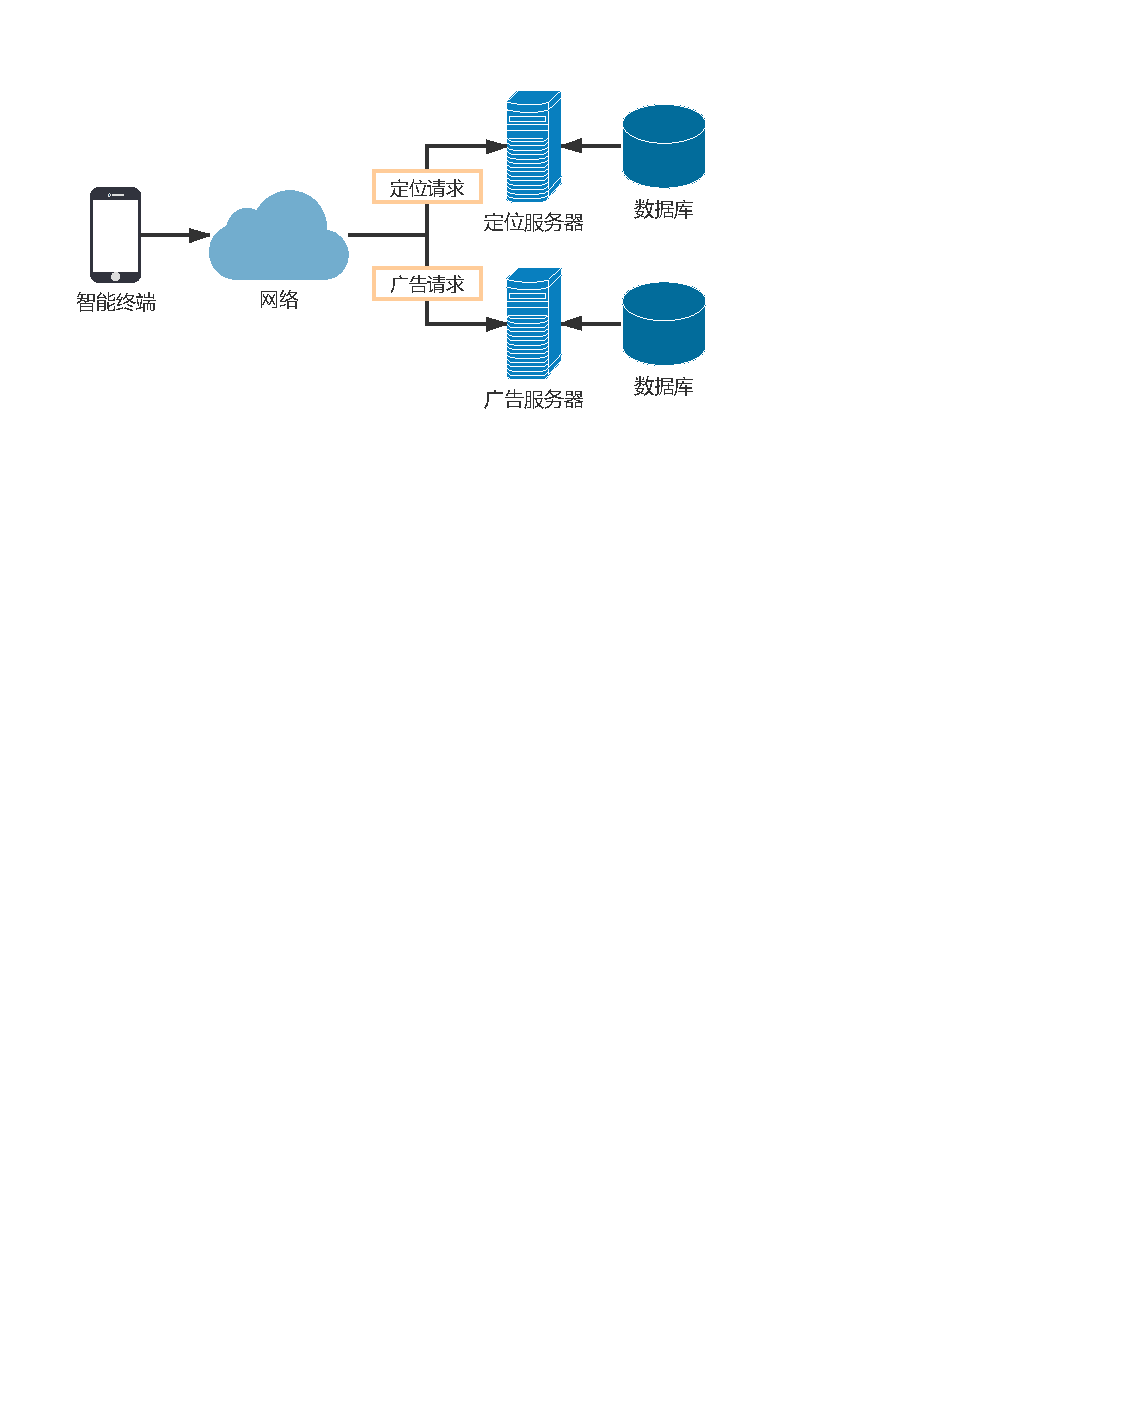
\includegraphics[width=\textwidth]{sys_arch.pdf}
	\caption{基于用户定位的广告投放服务机制的整体系统架构图。}
	\label{fig:sysarch}
\end{figure}

图\ref{fig:sysarch}所示为基于用户定位的广告投放系统总体框架。该系统由两大模块构成:定位服务模块和广告服务模块。每次用户访问该系统时,智能终端会先向定位服务器发送定位请求,定位服务器根据用户是信号发射源或接收端采取不同的算法计算用户位置,之后返回给终端。获得位置后,终端将向广告服务器发送广告请求,服务器计算完成后返回要投放给用户的广告。该系统主要由以下两个模块组成:
\begin{itemize}
	\item 在定位模块中,定位服务器其实是定位服务器群,因为这一部分由多个子模块组成,第\ref{sec:loc}节将详细介绍其系统架构和模块功能。如果终端是信号发射源,则数据库中存储着WAP接收到的该终端的RSS;若终端是信号接收端,则数据库中存储着历史上不同位置的RSS。从数据库中提取的数据被发送到定位服务器计算定位,最后位置被返回给终端。
	\item 在广告模块中,和定位模块类似,也是广告服务器群,第\ref{sec:ad}节将详细介绍其系统架构和模块功能。数据库存储着广告的具体内容,即视频、图片或文本形式的广告内容,在广告服务器决定要投放的广告之后到数据库提取相应的广告内容,并推送给用户。
\end{itemize}

当然图\ref{fig:sysarch}所展示的结构只是多种可能实现中的一种,比如定位信息的获取不是必须从定位服务器获取,也可以是在终端本地计算获得(比如卫星定位),只不过本文所提出的两种定位算法均需要在服务器计算获得定位信息。

\section{定位服务器系统架构} \label{sec:loc}

\begin{figure}[htb]
	\centering
	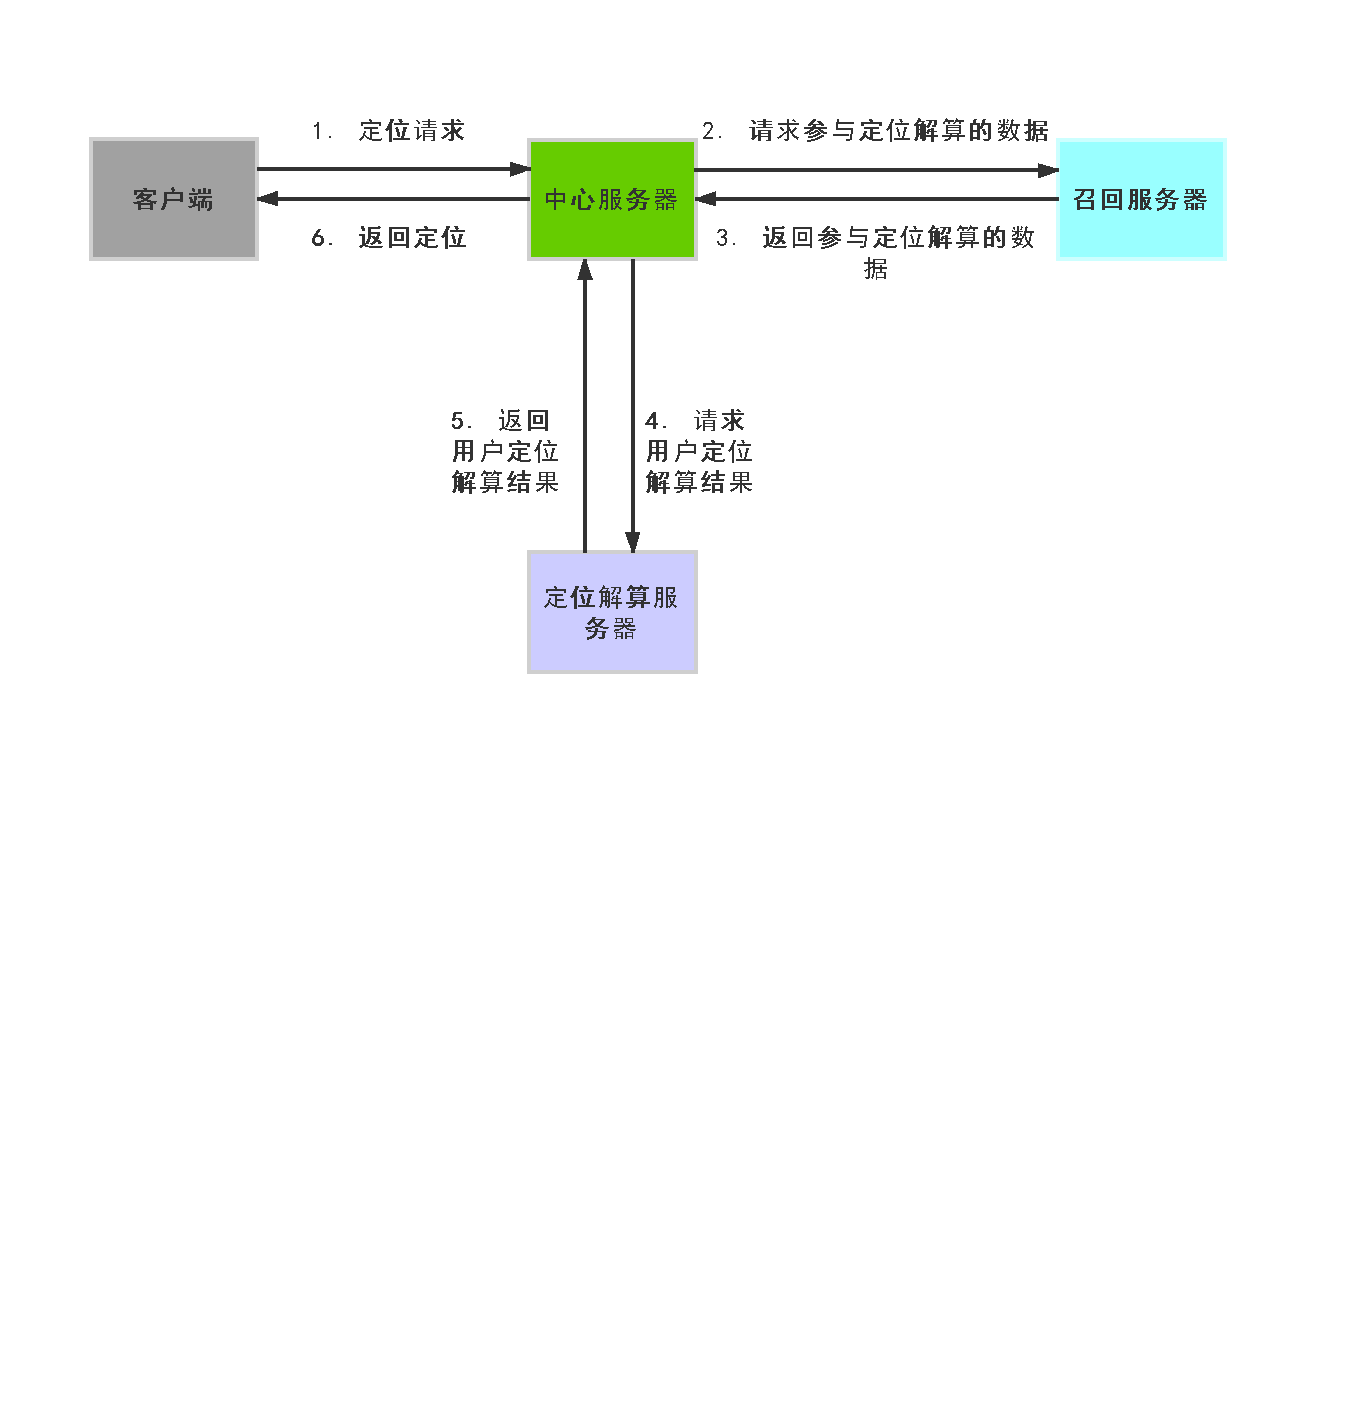
\includegraphics[width=\textwidth]{localization_process_cn.pdf}
	\caption{针对一次用户定位请求的工作流程图。}
	\label{fig:loc_sys}
\end{figure}

定位服务器(群)的具体结构如图\ref{fig:loc_sys}所示。每次客户端发起定位请求,中心服务器将依次从召回服务器取得数据、从定位解算服务器获取用户的定位信息,最后将用户位置返回终端。这里,中心服务器、召回服务器和定位解算服务器共同构成了定位服务器群。定位服务器依次执行的三步操作如下:
\begin{enumerate}
	\item 数据召回。由于数据库中数据量巨大,然而真正和当前用户定位相关的数据并没有那么多,因此我们需要设计一种快速算法将这些相关数据筛选出来。针对发射源定位和接收端定位的两种场景,我们将采用不同的召回策略:
	\begin{itemize}
		\item 发射源定位召回策略。由于发射源定位需要的用户周围基站处对于用户发射信号的RSS,而且数据库的写入会存在较大的延迟(相比于定位可以容忍的延迟),因此这里我们的策略是,当收到用户的定位请求后,令能接收到该用户信号的WAP将其RSS发送到中心服务器,则实现了数据的召回;
		
		\item 接收端定位召回策略。我们的接收端定位算法采用的是指纹定位,即利用附近WAP对用户的RSS与其所在区域的历史RSS数据进行匹配,用某种算法估计当前用户的位置。由于用户需要向定位服务器发送其RSS,因此我们知道用户能接收到哪些WAP的信号,据此可以在数据库中筛选出同时能够接收到这些WAP信号的点,或者适当放宽条件,可以接收到其中$1-\epsilon (0 < \epsilon < 1)$个WAP的点就被召回。这些数据将用作后续的匹配算法中;
	\end{itemize}
	
	\item 定位解算。这一部分是第\ref{cha:transmitter}章和第\ref{cha:fingerprint}章主要描述的内容,分别对应发射源定位和接收端定位。中心服务器将被召回的数据(如果是接收端定位,则还有用户的RSS数据)发送给定位解算服务器,根据定位的类型采取不同的算法解算用户位置。计算完成后,将用户位置返回给中心服务器;
	
	\item 最后,中心服务器通过网络将用户位置返回客户端。
\end{enumerate}

上述定位服务器架构只是一种可能的实现方式,比如当定位范围很小、数据较少的时候则可以省去数据召回的步骤,直接进行定位解算。这些其他的可能的架构在这里就不再赘述。

\section{广告服务器系统架构} \label{sec:ad}

\begin{figure}[htb]
	\centering
	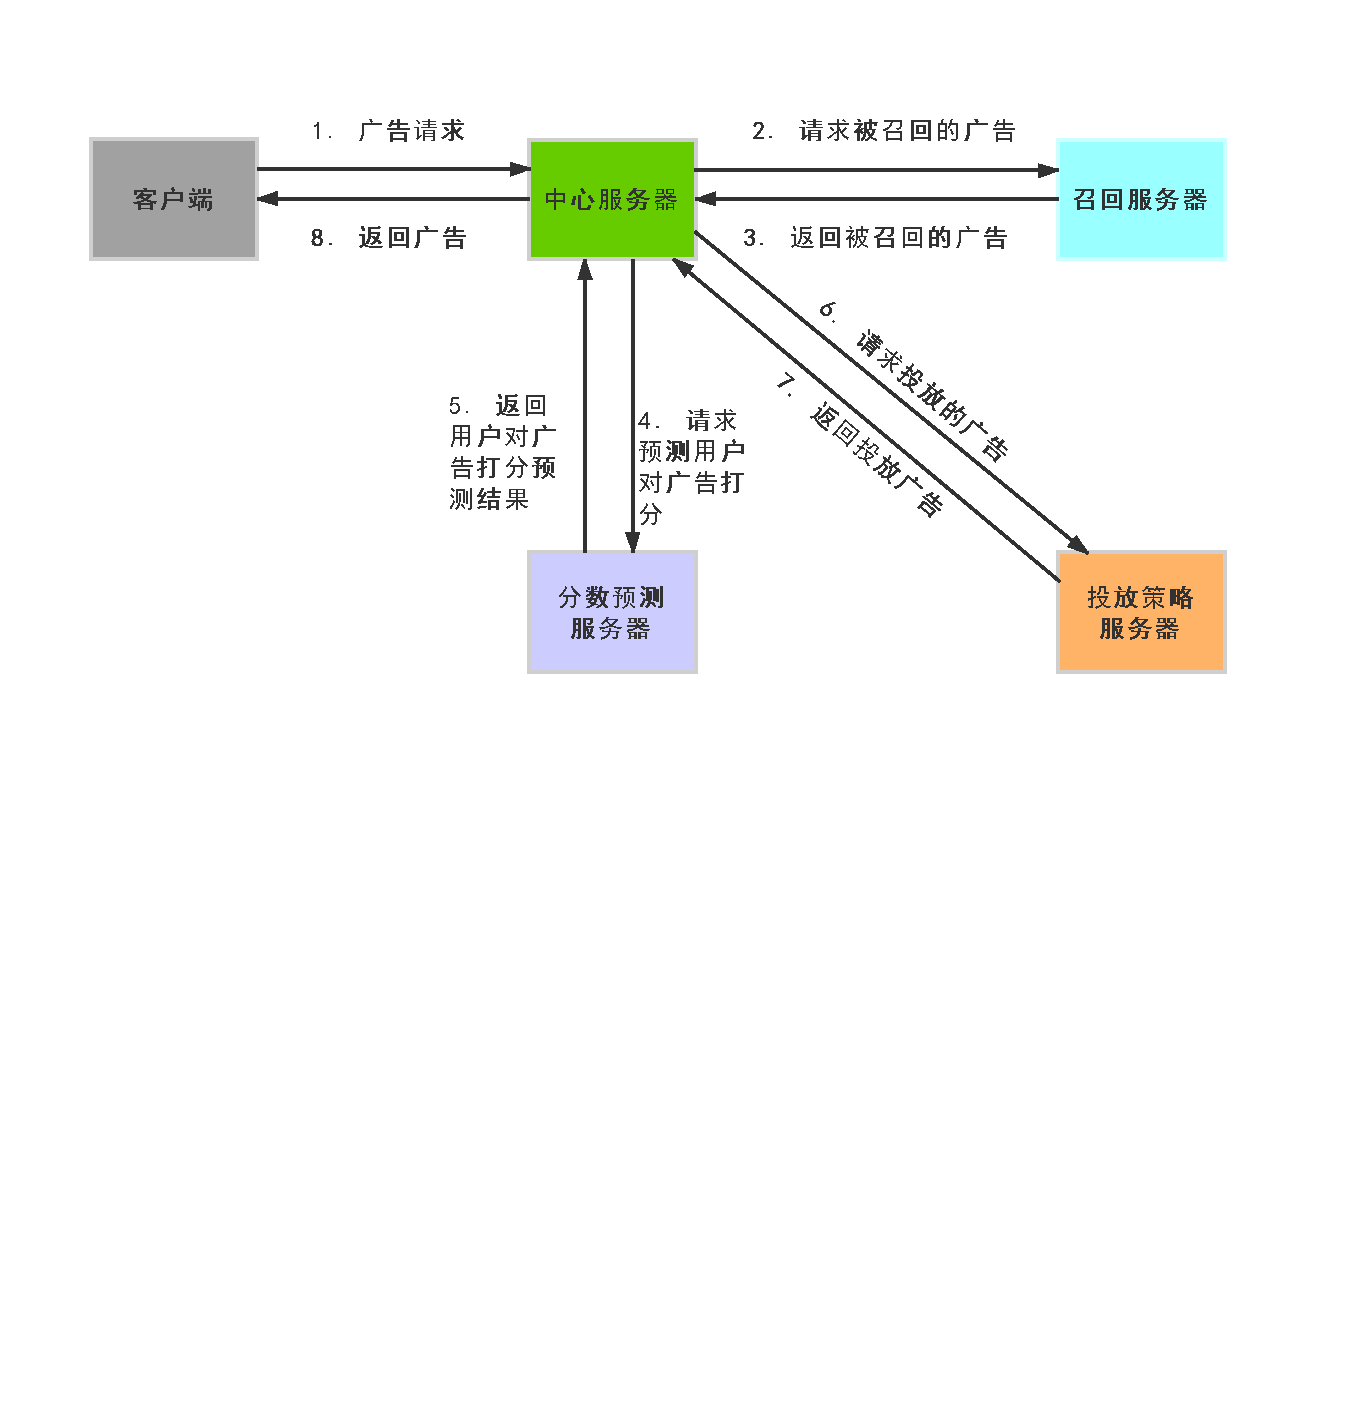
\includegraphics[width=\textwidth]{FansTop_process_cn.pdf}
	\caption{针对一次访问投放广告的工作流程图。}
	\label{fig:fssys}
\end{figure}

广告服务器(群)的具体结构如图\ref{fig:fssys}所示。流程从客户端发起广告请求开始,之后中心服务器依次请求召回广告、预测用户对被召回广告的打分和打算投放的广告。我们的算法将部署在投放策略服务器上。中心服务器、召回服务器、分数预测服务器和投放策略服务器共同构成了广告服务器群。广告服务器依次执行的四步操作如下:
\begin{enumerate}
	\item 广告召回。因为广告数量与服务器计算能力之间的矛盾,只有部分广告会参与后续流程,这个粗略过滤的操作被称作“召回”(Retrieval)或“候选集生成”(Candidate Generation)。不同于定位服务器中的召回服务,这里召回的是候选投放的广告,而定位中召回的相关、可以参与定位的历史数据。因为我们的算法要部署在同城页,这里仅介绍同城页的广告召回策略,即候选广告是根据访问用户与广告主之间的距离筛选的,也就是需要用到上文的定位信息。为了保证广告主得到他期望的曝光量,首先我们就得保证该条广告的召回量充足。为此,我们设置了几个距离等级,如果召回量太少就扩大召回范围,反之则缩小范围,使得广告召回量处在动态平衡中,既不会无法完成广告投放,又可以是得被投放广告的用户尽量靠近广告主;
	\item 分数预测。在被召回广告返回后,中心服务器会向分数预测服务器发送请求,以预测这些用户对于这些被召回广告的打分。预测服务器会根据广告特征、用户特征,以及用户过往行为等数据对当前广告预测分数。更详细的,预测服务器会返回CTR和条件关注率(Conditional Follow Rate, CFR)的线性组合:
	\begin{equation}
		score = CTR \times  (b + a \times CFR), \label{eq:score}
	\end{equation}
	其中 $a$ 和 $b$ 是线性组合系数,这里的条件关注率CFR是指在用户已经点击广告的条件下,用户关注广告主的概率,即分数可以被改写为:
	\begin{equation}
	score = b \times CTR + a \times FTR, 
	\end{equation}
	预测服务器会分别预测出\eqref{eq:score}中的CTR和CFR,之后返回分数。预测CFR而不是直接预测FTR的原因可能是一般FTR都比较小,直接预测的准确率较低;
	\item 投放广告,这也是第\ref{cha:allocation}章主要描述的部分。中心服务器在向投放策略服务器请求要投放的广告的同时,也会把召回的广告及其分数一起发送。计算完成后返回给中心服务器决定投放的广告。我们的算法和之前部署的流控算法唯一区别就在投放策略服务器上;
	\item 获取广告内容后,中心服务器将广告返回客户端。
\end{enumerate}

上述流程和框图是广告服务器的大致框架。限于篇幅原因,其他一些与算法无关的底层实现将不会在这里讨论。






\chapter{基于接收信号强度的几何模型发射源定位算法}
\label{cha:transmitter}

本章将要介绍基于接收信号强度的几何模型发射源定位算法,即用户作为信号发射源时实现对用户定位的算法。具体应用场景可以描述为:一个用户终端以恒定功率发射信号(比如蜂窝网或WLAN中用户上行通信),通信范围内的多个WAP(基站或是无线路由器)接收到信号并测得RSS,最后根据这些RSS实现对用户定位。

\section{路径损耗模型和估计器}

\subsection{路径损耗模型}

不妨设总共有$N$个WAP即信号接收者,则第$i$个接收者的RSS可用下式表示~\cite{erceg1999empirically}:
\begin{equation}
{P_i} = C - 10\alpha {\log _{10}}({\left\| {{\bm{\theta}} - {{\bm{\mathrm{x}}_i}}} \right\|_2}) + {n_i}, i = 1,2,...,N,\label{eq:rss}
\end{equation}
其中$P_i$是接收者的RSS,$\bm{\theta}$是发射源即用户的位置,$\alpha$是路径损耗指数,$C$是一个与$\bm{\theta}$ 和 $\bm{\mathrm{x}}_i$无关的常数,$n_i$则是均值为$0$、方差为${\sigma_i}^2$的高斯白噪声。为了简化表达,我们用下式代表发射源与接收端之间的距离:
\begin{equation}
d_i = {\left\| {{\bm{\theta}} - {{\bm{\mathrm{x}}_i}}} \right\|_2}, \forall i. \label{eq:d}
\end{equation}
因为$C$是常数,所以它可以通过与另一个接收者的RSS相减被消除,即:
\begin{equation}
{P_{ij}} = 10\alpha ({\log _{10}}d_j - {\log _{10}}d_i) + {n_{ij}}, i \neq j, \label{eq:diff_rss}
\end{equation}
其中$P_{ij} = P_i - P_j$,$n_{ij}$变为$0$均值、方差为$\sigma_i^2 + \sigma_j^2$的高斯白噪声。注意到,因为我们没有锚点,因此这里让$i$作为RSS最大的接收者的下标。为了使表达更清晰,在接下来的部分我们将用$\bm{\mathrm{x}}_M, d_M$代表$\bm{\mathrm{x}}_i, d_i$。

\subsection{传统最大似然估计器}

传统最大似然(Maximum Likelihood, ML)估计器通过求解如下优化问题从而找到定位$\bm{\hat{\theta}}$:
\begin{equation}
\widehat {\bm{\theta }} = \mathop {\arg \min }\limits_{\bm{\theta }} \sum\limits_{j = 1}^N {{{[{P_{Mj}} - 10\alpha ({{\log }_{10}}d_j - {{\log }_{10}}d_M)]}^2}}, j \neq M. \label{eq:ml}
\end{equation}
因为这是一个非凸优化问题,许多凸优化估计器(比如半正定规划)和线性最小二乘估计被提出,正如第\ref{cha:intro}章所述。因为ML估计器是作为算法比较基准线的,我们需要选择一个能够取得最小误差的作为基准,因此直接优化非凸的非线性最小二乘问题。为了尽可能找到最优解,我们会多次随机初始点,选择损失函数最小的作为最终定位。

\subsection{基于几何的模型}

S. Wang 和 R. Inkol~\cite{wang2011near} 提出了一种线性最小二乘估计器(Linear Least Square, LLS),在推导过程中发现每两个接收端RSS可以形成一个发射源坐落在其上的圆。但是这个结论没有被作者直接用来优化,而是提出了一种线性最小二乘法。接下来我们将用这个知识得到基于几何的模型(Geometry-Based Model, GBM)。

如果我们忽略\eqref{eq:diff_rss}中的噪声项,可以得到:
\begin{equation}
{P_{ij}} - 5\alpha {\log _{10}}({\dfrac{d_j}{d_i}})^2 = 0, i \neq j. \label{eq:ignore}
\end{equation}
令:
\begin{equation}
\gamma = 10^{\frac{P_{ij}}{5\alpha}}, \label{eq:gamma}
\end{equation}
则\eqref{eq:ignore}可以被改写为:
\begin{equation}
{\left\| {\bm{\theta}  - \bm{\mathrm{x}}_j} \right\|_2}^2 = {\gamma _{ij}}{\left\| {\bm{\theta}  - \bm{\mathrm{x}}_i} \right\|_2}^2. \label{eq:10exp}
\end{equation}
如果 $\gamma _{ij} \neq 1$,即两个接收端的RSS不相等,\eqref{eq:10exp}可以被改写为:
\begin{equation}
{\left\| {\bm{\theta}  - \frac{\bm{\mathrm{x}}_j - \gamma_{ij}\bm{\mathrm{x}}_i}{1 - \gamma_{ij}}} \right\|_2}^2 = \frac{\gamma_{ij}{d_{ij}}^2}{(1 - \gamma_{ij})^2}, \label{eq:circle}
\end{equation}
其中$d_{ij} = \left\| \bm{\mathrm{x}}_i  - \bm{\mathrm{x}}_j \right\|_2$。显然这是一个$\bm{\theta}$坐落在其边缘上的圆,而圆心和半径分别为:
\begin{equation}
\bm{\mathrm{o}}_j = \frac{\bm{\mathrm{x}}_j - \gamma_{ij}\bm{\mathrm{x}}_i}{1 - \gamma_{ij}}, {r_j}^2 = \frac{\gamma_{ij}{d_{ij}}^2}{(1 - \gamma_{ij})^2}. \label{eq:oR}
\end{equation}

让$i$座位最大RSS接收端的下标(如果有多于1个最大RSS,则随机挑选一个而提出其余的)并用$M$替换$i$。假设\eqref{eq:circle}被下面的加性噪声影响:
\begin{equation}
{\left\| {\bm{\theta}  - o_j} \right\|_2}^2 = d_j + n_j, j \neq M, \label{eq:GBMnoise}
\end{equation}
其中$n_j$是一个服从均值为$0$、方差为$\sigma_j^2$的截断高斯分布的噪声。因为$\bm{\theta}$是实数,因此\eqref{eq:GBMnoise}等式右边必须大于等于$0$,即$n_j$的取值范围是 $[-d_j, +\infty)$。所以我们建立了一个带有噪声$n_j$的模型,服从截断高斯分布。注意到这里的$n_j$与\eqref{eq:rss}中的噪声无关,因为这是两个独立的模型。

利用上述模型,我们可以定义一个服从截断高斯分布的随机变量$X_j = \left\|{\bm\theta} - \bm{\mathrm{o}}_j\right\|_2$,其概率密度函数是:
\begin{equation}
f(x_j) = \frac{1}{C(r_j)}\exp(-\frac{(x_j - r_j)^2}{2{\sigma_j}^2})I[0, +\infty), \label{eq:pdf}
\end{equation}
其中 $C(r_j) = \int_0^{ + \infty }\exp(-\frac{(x_j - r_j)^2}{2{\sigma_j}^2})dx_j$是归一化系数,$I[0, +\infty)$是指示函数,在$[0, +\infty)$范围内取值$1$其余为$0$。

因此,最终的损失函数和优化问题可以表示为:
\begin{equation}
\widehat {\bm{\theta }} = \mathop {\arg \min }\limits_{\bm{\theta }} \frac{1}{2}\sum\limits_{j = 1}^{N^-} {\frac{1}{\sigma_j^2}(\left\|{\bm\theta} - \bm{\mathrm{o}}_j\right\|_2 - r_j)^2}, \label{eq:loss}
\end{equation}
其中$N^-$代表剩余的接收端数量。因为$C(r_j)$和$\bm\theta$无关,因此在优化时可以忽略。

当假设所有接收端的噪声方差$\sigma_j^2$相同时,该优化问题就变成找到一个点,使得它到所有圆边缘的距离之和最小。因此这个优化问题有着清楚的几何意义,于是我们把\eqref{eq:loss}称为基于几何的模型(Geometry-Based Model, GBM)。

因为无法证明GBM的凸性,我们将采用和ML中相同的方法求解,即多次随机挑选初始点后选取使得损失函数最小的结果。

后续的仿真结果表明GBM估计器是有偏的。但是注意到,我们的目标是最小化均方根误差(Mean Square Error, MSE)而MSE可以写作:
\begin{equation}    \label{eq:mse}
\begin{split}
MSE &= \mathrm{E}[(\widehat{\theta} - \theta)^2]\\
&= (\mathrm{E}[\widehat{\theta}] - \theta)^2 + \mathrm{E}[(\widehat{\theta} - \mathrm{E}[\widehat{\theta}])^2]\\
&= bias^2 + variance.
\end{split}
\end{equation}
即MSE是由估计器的偏差的平方和方差两部分组成,这也是机器学习领域经常出现的经典问题。若一个估计器有很小的偏差却有很大的方差则被称为“过拟合”(Over-Fitting)。在仿真和实测数据验证部分,我们会展示传统最大似然估计器相比于GBM是过拟合的。

\section{克拉美罗下界(Cram\'{e}r-Rao Lower Bound, CRLB)}

CRLB是估计器的理论误差下界,虽然不一定能够达到,但是对其进行分析有助于研究估计器的性能。

\subsection{无偏估计的CRLB}

对于路径损耗模型,因为第$i$个接收端的RSS的分布服从$p_i \sim \mathcal{N}(-10\alpha\mathrm{log}_{10}{d_i} -C, {\sigma_i}^2)$,因此费舍信息(Fisher Information)可表示为:
\begin{equation}
I(\bm{\theta}) = (\frac{10\alpha}{\sigma\mathrm{ln}10})^2\sum\limits_{i = 1}^N(\frac{{\bm\theta} - \bm{\mathrm{x}}_i}{{\left\|{\bm\theta} - \bm{\mathrm{x}}_i\right\|_2}^2})(\frac{{\bm\theta} - \bm{\mathrm{x}}_i}{{\left\|{\bm\theta} - \bm{\mathrm{x}}_i\right\|_2}^2})^T, \label{eq:fisher}
\end{equation}
其中$\sigma$是噪声的标准差。如果估计器是无偏的,则协方差矩阵的CRLB为:
\begin{equation}
\begin{split}
CRLB(\bm{\theta}) &= I(\bm{\theta})^{-1} \label{eq:unbias_cov}\\
&\le Cov(\widehat{\bm{\theta}}_{ML}).
\end{split}
\end{equation}

因为最大似然估计器是渐进无偏的~ \cite{kay1993fundamentals},根据\eqref{eq:mse},最大似然法的RSME的估计下界可以表示为:
\begin{equation}
RMSE \ge \sqrt{Tr(CRLB)},\label{eq:rmse_ml}
\end{equation}
其中$Tr(\cdot)$是矩阵的迹,即对角线元素累加。

\subsection{有偏估计的CRLB}

假设GBM估计器的期望是$\bm\phi(\bm{\theta})$,如果估计器有偏,则协方差矩阵的CRLB可由下式所得:
\begin{equation}
\begin{split}
CRLB_{GBM}(\bm{\theta}) &= {\frac{\partial\bm\phi(\bm{\theta})}{\partial \bm\theta}}I(\bm{\theta})^{-1}{\frac{\partial\bm\phi(\bm{\theta})}{\partial \bm\theta}}^T\\
& \le Cov(\widehat{\bm{\theta}}_{GBM}),
\end{split}
\end{equation}
其中$\frac{\partial\bm\phi(\bm{\theta})}{\partial \bm\theta}$是雅可比(Jacobian)矩阵。注意到如果估计器是无偏的,则$\bm\phi(\bm{\theta}) = \bm{\theta}$即$\frac{\partial\bm\phi(\bm{\theta})}{\partial \bm\theta} = \bm{I}$,而这与\eqref{eq:unbias_cov}一致。

根据\eqref{eq:mse},GBM的RMSE的下界可表示为:
\begin{equation}
RMSE\! \ge\! \sqrt{{(\bm\phi(\bm{\theta})\! -\! \bm{\theta})}^T(\bm\phi(\bm{\theta})\! -\! \bm{\theta})\! +\! \mathrm{Tr}(CRLB_{GBM}(\bm{\theta}))}.\label{eq:rmse_gbm}
\end{equation}

直接计算$\bm\phi(\bm{\theta})$ 和 ${\frac{\partial\bm\phi(\bm{\theta})}{\partial \bm\theta}}$较困难,但是我们知道接收者RSS的分布,因此蒙特卡洛法适用于该问题。

首先,$\bm\phi(\bm{\theta})$比较容易用下式得到:
\begin{equation}
\begin{split}
\bm\phi(\bm{\theta}) &= \mathrm{E}[\widehat{\bm{\theta}}]\\
&\approx \frac{\sum\limits_{k = 1}^K{\widehat{\bm{\theta}}}}{K},
\end{split}
\end{equation}
其中,$K$是仿真次数。${\frac{\partial\bm\phi(\bm{\theta})}{\partial \bm\theta}}$可以直接用有限差分法得到,但是这可能需要大量时间计算,因为我们需要在二维平面内多次用不同的$\bm\theta$进行仿真。

接下来,我们将推导一种不需要用不同的$\bm\theta$仿真就可以得到${\frac{\partial\bm\phi(\bm{\theta})}{\partial \bm\theta}}$的方法。首先 $\bm\phi(\bm{\theta})$可以用如下公式表示:
\begin{equation}
\begin{split}
&Let \quad f(\bm{\theta}) = {\prod\limits_{i=1}^N}(2\pi{\sigma_i}^2)^{-\frac{1}{2}}e^{-\frac{(p_i + 10\alpha\mathrm{log}_{10}{d_i} + C)^2}{2{\sigma_i}^2}},\\
&then \quad \bm\phi(\bm{\theta}) = \iiint_{\mathbb{R}^N}\widehat{\bm{\theta}}f(\bm{\theta})dp_1...dp_N,
\end{split}
\end{equation}
其中$d_i$由\eqref{eq:d}定义。若$\widehat{\bm{\theta}}f(\bm{\theta})$ 和 $\frac{\partial \widehat{\bm{\theta}}f(\bm\theta)}{\partial \bm{\theta}}$是连续的,$\iiint_{\mathbb{R}^N}\widehat{\bm{\theta}}f(\bm\theta)$ 和 $\iiint_{\mathbb{R}^N}\frac{\partial \widehat{\bm{\theta}}f(\bm\theta)}{\partial \bm{\theta}}$一致收敛,则
\begin{equation}
\begin{split}
{\frac{\partial\bm\phi(\bm{\theta})}{\partial \bm\theta}} &= \frac{\partial\mathrm{E}[\widehat{\bm{\theta}}]}{\partial \bm{\theta}}\\
&= \frac{\partial}{\partial \bm{\theta}}\iiint_{\mathbb{R}^N} \widehat{\bm{\theta}}f(\bm{\theta}) dp_1...dp_N\\
&= \iiint_{\mathbb{R}^N} \frac{\partial \widehat{\bm{\theta}}f(\bm{\theta})}{\partial \bm{\theta}} dp_1...dp_N\\
&= \iiint_{\mathbb{R}^N} \sum\limits_{i=1}^N \widehat{\bm{\theta}}(\frac{-10\alpha}{{\sigma_i}^2\mathrm{ln}10}\frac{{\bm\theta} - \bm{\mathrm{x}}_i}{{\left\|{\bm\theta} - \bm{\mathrm{x}}_i\right\|_2}^2})^Tf(\bm{\theta}) dp_1...dp_N\\
&= \mathrm{E}[\sum\limits_{i=1}^N\widehat{\bm{\theta}}(\frac{-10\alpha}{{\sigma_i}^2\mathrm{ln}10}\frac{{\bm\theta} - \bm{\mathrm{x}}_i}{{\left\|{\bm\theta} - \bm{\mathrm{x}}_i\right\|_2}^2})^T]. \label{eq:mc}
\end{split}
\end{equation}
需要注意$\widehat{\bm{\theta}}$与$\bm{\theta}$无关,而是关于$(\bm{\mathrm{x}}_1,...,\bm{\mathrm{x}}_N)^T$ 和 $(P_1,...,P_N)^T$的函数。

根据\eqref{eq:mc}的结果,我们可以通过计算$\sum\limits_{i=1}^N\widehat{\bm{\theta}}(\frac{-10\alpha}{{\sigma_i}^2\mathrm{ln}10}\frac{{\bm\theta} - \bm{\mathrm{x}}_i}{{\left\|{\bm\theta} - \bm{\mathrm{x}}_i\right\|_2}^2})^T$的经验平均值来利用蒙特卡洛法近似估算 ${\frac{\partial\bm\phi(\bm{\theta})}{\partial \bm\theta}}$,而不需要有限差分,这会大量节省仿真时间。

\section{RMSE的置信区间}

估计器的精度会受到噪声的影响,因此为了判断不同的估计器是否统计显著地不同,我们需要计算RMSE的置信区间(Confidence Interval)。

虽然RMSE的分布未知,但是幸运地,依据中心极限定理(Central Limit Theorem),当仿真次数很多且$({\widehat{\bm{\theta}}_k - \bm{\theta}})^T({\widehat{\bm{\theta}}_k - \bm{\theta}})$对于不同的$k$来说独立同分布,则MSE的分布将会趋近于正态分布,即
\begin{equation}
\begin{split}
\mathop{\mathrm{lim}}\limits_{K\rightarrow\infty}MSE &= \mathop{\mathrm{lim}}\limits_{K\rightarrow\infty} \frac{\sum\limits_{k=1}^K({\widehat{\bm{\theta}}_k - \bm{\theta}})^T({\widehat{\bm{\theta}}_k - \bm{\theta}})}{K} \\
&\sim \mathcal{N}(\mu, \frac{\sigma^2}{K}),
\end{split}
\end{equation}
其中$\mu$ 和 ${\sigma}^2$ 是 $({\widehat{\bm{\theta}}_k - \bm{\theta}})^T({\widehat{\bm{\theta}}_k - \bm{\theta}})$的期望和方差。因为我们不知道方差和期望,所以应当使用经验均值代替期望,即我们应当使用T检验。但是,在仿真次数足够多的情况下(在我们的场景下仿真了100,000次),我们可以直接使用Z检验。因此$95\%$置信区间可由下式获得:
\begin{equation}
CI = (\sqrt{RMSE^2 - 1.96\frac{\sigma}{\sqrt{K}}}, \sqrt{RMSE^2 + 1.96\frac{\sigma}{\sqrt{K}}}). \label{eq:ci}
\end{equation}
因此我们可以用\eqref{eq:ci}得到RMSE的置信区间并检验两个估计器的RMSE是否统计显著的不同。

\section{数值仿真实验}

\subsection{仿真场景与估计器设置}

为了比较基于几何的模型(GBM),最大似然法(ML)以及线性最小二乘(LLS)估计器,我们进行了仿真实验。仿真场景设置与S. Wang 和 R. Inkol~\cite{wang2011near} 的场景相同:发射源坐标为(0, 0),十个接收者的位置坐标为 (-126, 62), (-339, 166), (390, 76), (-178, 333), (482, 122), (-234, 141), (230, -45), (-352, 279), (-104, 465), (366, -139)。上述坐标的单位是米,分布如图\ref{fig:simscene}所示。在生成接收信号数据时,路径损耗系数$\alpha=4$,噪声服从0均值高斯分布,方差从1变化到15,常数$C=-40$。

\begin{figure}
	\centering
	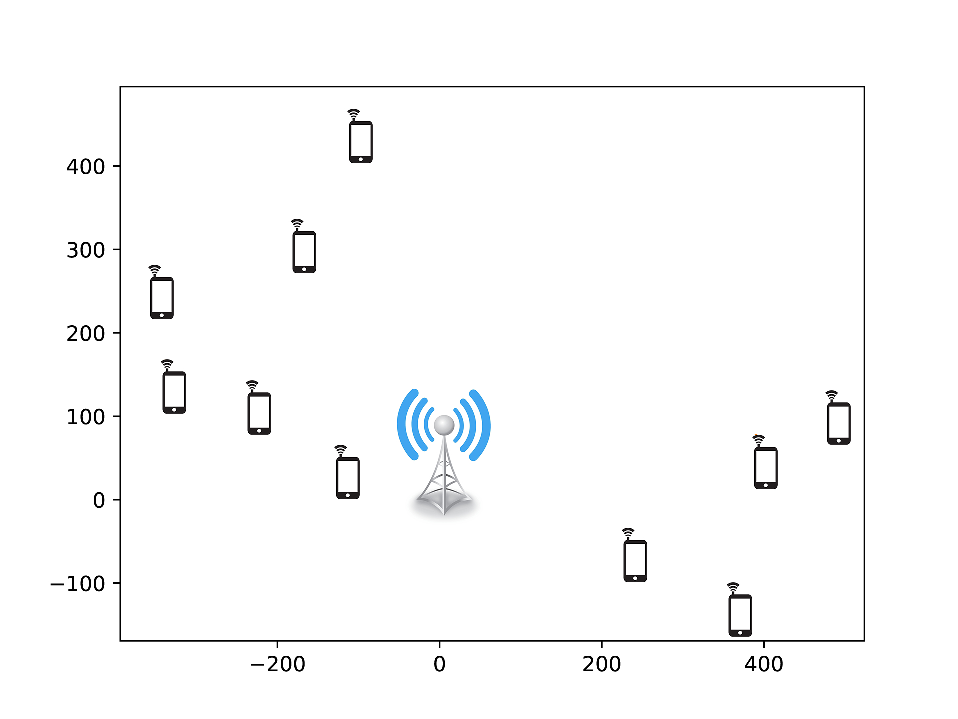
\includegraphics[width=\textwidth]{SimScene.pdf}
	\caption{发射源坐标为(0, 0),十个接收者的位置坐标为 (-126, 62), (-339, 166), (390, 76), (-178, 333), (482, 122), (-234, 141), (230, -45), (-352, 279), (-104, 465), (366, -139)。}
	\label{fig:simscene}
\end{figure}

因为GBM和ML都是非凸优化,因此我们将会以随机初始点进行20次迭代计算,使损失函数取得最小值的点作为最终定位点。初始点的二维坐标是从两个独立同分布的均匀分布$\mathcal{U}(-500, 500)$中采样所得。注意到我们的场景中没有锚点,因此必须选择一个接收端作为被减数,这里我们选择RSS最大的点。对于GBM,如果有多个最大值,则随机选择一个,其余的删除。GBM算法中的$\sigma_j$均被设为1。针对每个噪声方差,GBM、ML和LLS三种算法都仿真100,000次,之后计算RMSE及其置信区间。此外,无偏估计的CRLB以及GBM的CRLB分别根据\eqref{eq:rmse_ml}和\eqref{eq:rmse_gbm}计算。

\subsection{仿真结果}

\begin{figure}
	\centering
	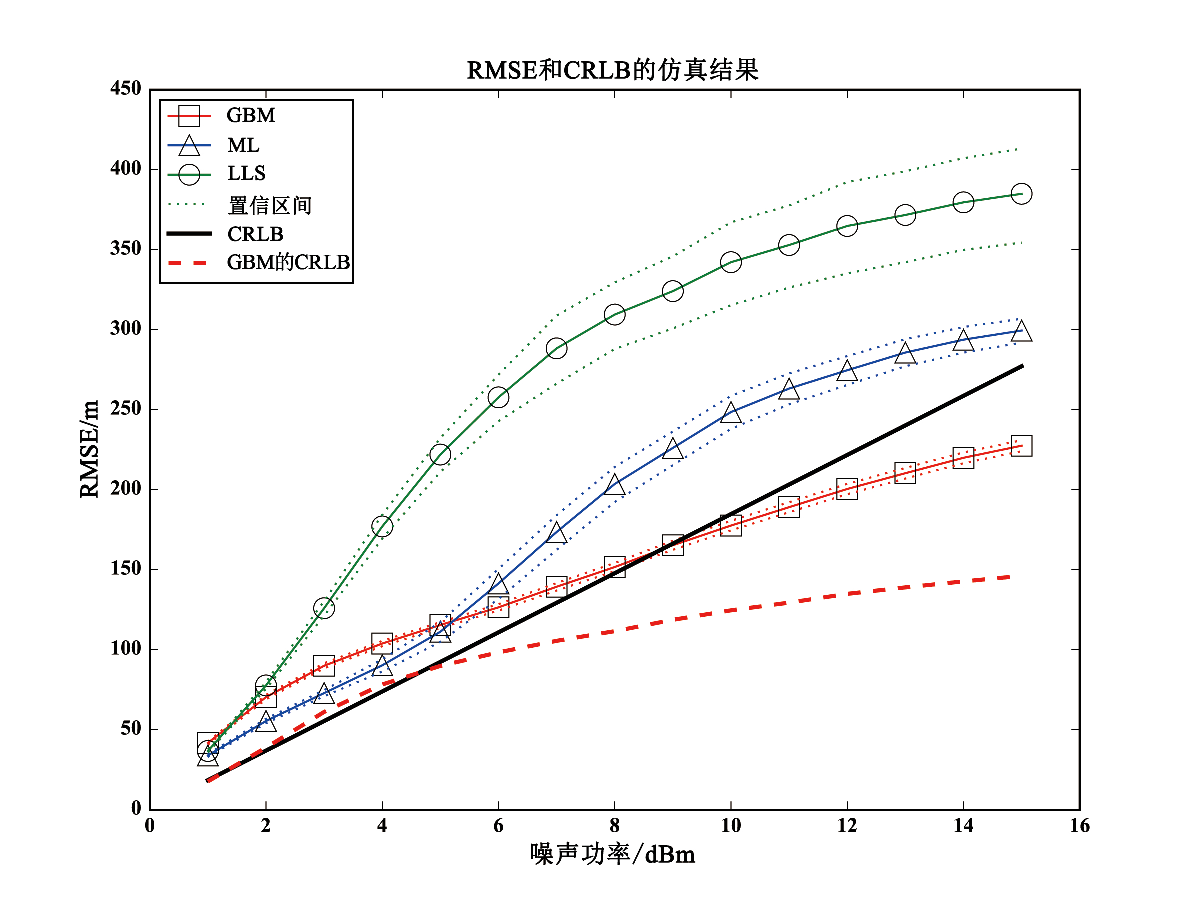
\includegraphics[width=\textwidth]{GBM_simulation.pdf}
	\caption{100,000次仿真下,RMSE、置信区间和CRLB的结果。正方形是我们的算法GBM,上三角是ML,圆圈是LLS。点线为RMSE的95\%置信区间。实线是无偏估计的CRLB,虚线是通过蒙特卡洛法估计的GBM的CRLB。}
	\label{fig:gbm_sim}
\end{figure}

如图\ref{fig:gbm_sim}所示为100,000次仿真下,RMSE及其95\%置信区间和CRLB的结果。从仿真结果中可以看到,当噪声标准差$\sigma<5$dBM时ML的RMSE略低于GBM。然而当标准差$\sigma>5$dBM时,GBM的RMSE明显小于ML而且统计显著。因为多径效应和阴影效应的影响,真实世界场景中往往噪声功率较大。下一小节中,我们将上述三种算法用于实测数据,结果将为我们提供一些深入的见解。除此之外,CRLB的结果和GBM与ML的情况相似。虽然GBM的CRLB比它的RMSE小得多,但是我们不知道是否存在一种估计器可以取得这个下界。这或许是下一步研究的可能突破点。

注意到,当噪声的标准差大于9之后,GBM的RMSE会比无偏估计的CRLB还低,这也暗示了GBM是有偏估计否则CRLB是RMSE的下界。根据\eqref{eq:mse},即虽然GBM是有偏估计,但是相比于方差的减小,偏置的稍微增加也不会使得总体MSE更大。从机器学习的角度来看,ML是一个低偏置、高方差的估计器,也就是说ML对于路径损耗模型“过拟合”了。而GBM类似于一种正则化版本,能够更好地适应高噪声数据。

最后,LLs估计器的RMSE最大。相比于LLS,ML能取得更小的RMSE已经被验证过~\cite{jackson2011received},而且当噪声较大时,LLS的性能会严重恶化~\cite{vaghefi2013cooperative}。我们的仿真结果与这些前人的结论一致。

\subsection{实测数据验证}

为了验证仿真结果并检测算法的在实际问题上的可用性,我们也采集了一些实测数据,根据接收信号强度对发射源定位。虽然我们算法设计的初衷是对用户定位,但是其实只要是信号发射源即可。因此为了数据采集的便利,我们的数据采集的是商用蜂窝网内基站的发射信号,车载路测仪作为接收端在小区内的道路上采集数据。

\subsubsection{数据介绍}

数据由车载路测仪在城市街道内运行采集移动通信基站的接收信号强度,其中共有超过120,000个基站。路测仪每$5s$采集一次GPS定位坐标、RSS、LAC (Location Area Code)、CID (Cell ID) 以及其他的基站信息。为了尽量最小化遮挡对信号衰减造成的影响,我们选择GSM(Global System for Mobile)信号用作测试。GSM的信号频段是900MHz和1.8GHz。

在定位之前,数据需要经过预处理。首先,将GPS的经纬度坐标转换为笛卡尔直角坐标系。其次,为了减少计算时间并降低阴影效应的影响,RSS$<-60$dBM的点将被删除。最后,满足如下要求的基站(发射源,目标定位点)将被选中进行实验:
\begin{itemize}
	\item 信号制式是GSM;
	\item 在基站的可接收范围内有至少10个接收点;
	\item 距离基站最近的接收点距离基站的距离小于1000m。
\end{itemize}

经过筛选后,共有17321个可用基站,这些数据将被用于实验。经过统计,这些基站的平均辐射半径为751m,即最小RSS对应的接收位置与基站之间的距离的平均值。后续的三个估计器的路径损耗系数$\alpha$均被设为4。

\subsubsection{实测数据实验结果}

\begin{table}[tbp]
	\caption{实测数据实验结果}
	\begin{center}
		\begin{tabular}{cccc}
			\toprule
			\textbf{估计器} & \textbf{GBM} & \textbf{ML} & \textbf{LLS} \\
			\midrule
			\textbf{RMSE} [m] & 367.52 & 453.33 & 4898.10 \\
			\midrule
			\textbf{MAE}$^{a}$ [m] & 282.43 & 380.08 & 936.19 \\
			\bottomrule
			\multicolumn{3}{l}{$^{\mathrm{a}}$Mean Absolute Error.}
		\end{tabular}
		\label{tab:transmitter}
	\end{center}
\end{table}

如表\ref{tab:transmitter}所示,相比于ML和LLS,GBM可以在RMSE和MAE(Mean Absolute Error,平均绝对值误差)上均取得更小的误差。其中MAE由下式计算:
\begin{equation}
MAE = \frac{\sum\limits_{k=1}^K{\left\| \widehat{\bm{\theta}} - \bm{\theta} \right\|}_2}{K}.
\end{equation}

根据仿真结果,即当噪声较大时GBM的定位误差明显小于ML,我们可以发现实测数据受噪声影响较大,因此GBM能取得小得多的定位误差。GBM的定位误差比ML的误差低将近100m,相对的,RMSE上降低了23.35\%,MAE上降低了34.75\%。从实验结果中我们可以发现,相比于ML,GBM更适用于在实际的商用无线网络中对发射源定位,因为真实环境噪声很大。此外,LLS的定位误差确认了前人工作中的论述,即LLS估计器的定位效果在噪声较大时会严重恶化。

\subsection{本章小结}

本章中,我们提出了一种基于接收信号强度的,利用几何模型对发射源定位的算法。除此之外,一种节省计算时间的、利用蒙特卡洛法估计GBM的RMSE的克拉美罗下界的方法也被提出,同时给出基于中心极限定理计算RMSE的置信区间的方法。仿真实验显示,相比于ML,在噪声方差较大时GBM算法可以取得高得多的定位精度,即意味着GBM更加稳健。无偏估计的CRLB和GBM的CRLB呈现出和上述现象相似的结果。为了验证仿真结果并测试算法实用性,我们还从商用蜂窝网内采集数据进行测试。实验结果显示,GBM在RMSE和MAE上均取得更小的定位误差,这个结果或许说明GBM更适用于真实场景下的发射源定位需求。







\chapter{基于曼哈顿切线距离的指纹定位算法}
\label{cha:fingerprint}

本章将介绍基于曼哈顿切线距离的指纹定位算法,用户作为无线蜂窝网或者Wi-Fi信号的接收端,根据接收信号强度实现对自身的定位。虽然信号是在用户终端收集的,但是不必限制定位的解算也必须在本地完成,也可以将收集的信号上传云端,服务器端解算完成后返回给终端。本章所提出的算法就是一种需要在云端完成计算的算法。

\section{指纹定位中的常用距离度量方式}

指纹定位是基于一种假设,即在物理空间中邻近的两点,在信号空间中的距离也应较短,反之亦然,因为物理上相邻的两点应有相似的信道信息和多径效应。所以,如果从多个不同WAP发射信号的RSS已知,物理位置应该可以通过在信号空间中与历史数据运算估算出当前位置。K近邻(K-Nearest Neighbors, KNN)算法是一种常见的用于指纹定位的机器学习算法,通过在信号空间中找出最近的k的点并以某种方式对这k个点的物理位置组合后得到估测的定位。本文所采用的的算法是加权KNN(Weighted-KNN),即以信号空间中距离的倒数作为权重对物理位置加权平均得到定位。KNN算法中最明显的可调节参数就是近邻数k,但是既然近邻是由距离度量的,因此距离度量方式也应当被认真选择。

\subsection{常见度量方式}

首先,让我们定义一个物理-信号空间对:$(\mathbf{x}, \mathbf{s})$,其中$\mathbf{x}$是物理空间坐标,$\mathbf{s})$是不同WAP到终端的RSS向量。不妨假设$D$代表信号向量$\mathbf{s}$的维度。

正如第\ref{cha:intro}章中所说,欧氏距离、曼哈顿距离和余弦相似度是指纹定位中一些常用的度量方式。

欧氏距离和曼哈顿距离都属于明可夫斯基距离(Minkowski Distance),由下式定义:
\begin{equation}
d_{minkowski}(\mathbf{s}, \mathbf{r}) = \left(\sum_{i=1}^{D} {{\left| s_i - r_i \right|}^p}\right)^{\frac{1}{p}}, \label{eq:minkowski}
\end{equation}
其中$\mathbf{s}, \mathbf{r}$是两点的RSS向量。欧氏距离中$p=2$,曼哈顿距离中$p=1$。

经典余弦相似度由下式定义:
\begin{equation}
Cosine(\mathbf{s}, \mathbf{r}) = \frac{\mathbf{s}^T\mathbf{r}}{\left\|\mathbf{s}\right\|\left\|\mathbf{r}\right\|}, \label{eq:cosine}
\end{equation}
其取值于$[-1, 1]$区间,并且该值越接近1,则两个向量越相似,但是这与距离相反,因此我们将以$1 - Cosine(\mathbf{s}, \mathbf{r})$作为度量。

上述3种度量方式将被纳入考量范围,以比较它们的定位误差RMSE。第\ref{sec:exp}节的结果显示,在这些度量方式中,曼哈顿距离能取得最小的RMSE。

\subsection{常用度量方式的弊端}

虽然上述距离度量方式在指纹定位中被广泛应用,但是它们仍然有一些弊端会降低定位精度:
\begin{itemize}
	\item 不同RSS的信号共享相同的权重,这不是一个合理的选择。根据对数距离路径损失函数,在噪声相同的情况下,当RSS较大时,由噪声带来的从WAP到移动终端距离的扰动会小于RSS较小时。比如,同样是由噪声带来1dBM的RSS下降,在RSS较大时反应到距离上的改变就小于RSS较小时。因此,基于较大RSS较大的权重是一种合理的选择。注意到以dBM为单位的信号是自然信号取对数后的结果,那么我们可以逆向这个过程以给予大RSS更大的权重:
	\begin{equation}
	f(\mathbf{s}) = \mathrm{10}^{\frac{\mathbf{s}}{10\lambda}}, \label{eq:exp}
	\end{equation}
	其中$\lambda$是一个控制RSS权重的参数。$\lambda$越小,更大的相对权重会给予大的RSS。如果$\lambda$过小则会使得小的RSS在距离计算中被忽略,而如果$\lambda \rightarrow \infty$则会使得所有RSS的$f(\mathbf{s})$都一样。最终$f(\mathbf{s})$将作为信号空间中的数据,即基于$f(\mathbf{s})$计算K近邻。
	
	巧合的是,这个做法的效果已经被实验证实了~\cite{torres2015comprehensive}。但是,这篇文章没有分析$\lambda$对定位精度的影响,我们的实验结果将在第\ref{sec:exp}节中被展示;
	
	\item 流形的存在。如第\ref{cha:intro}章所述,流形是一个机器学习中的经典假设。样本的微小变化会形成流形,而在指纹定位中,物理空间中邻近的点的RSS应当居于信号空间中的一个流形上,因为局部的小区域应当拥有相似的信道信息而且变化较小。除此之外,在我们的数据集中,可接收信号的基站数量从80到200个不等,相比于二维物理空间,这是一个高维输入,而一般高维数据都居于低维流形上。当流形存在于高维空间中时,两点之间的距离应当是两点所在流形之间的距离而不是简单的距离度量所能表示的。
	
	在流行存在的情况下,如果一个测试点想被准确的分类或者回归,一个简单但低效甚至不可能实现的做法是采集所有可能情况下的数据,这样流形可以自动形成,从而简单度量也可以计算出流形之间的距离。但是,现实中数据集的大小受限,因此需要一种用有限数据估计流形之间距离的算法。
\end{itemize}

\section{指纹定位中的切线距离}

\begin{figure}
	\centering
	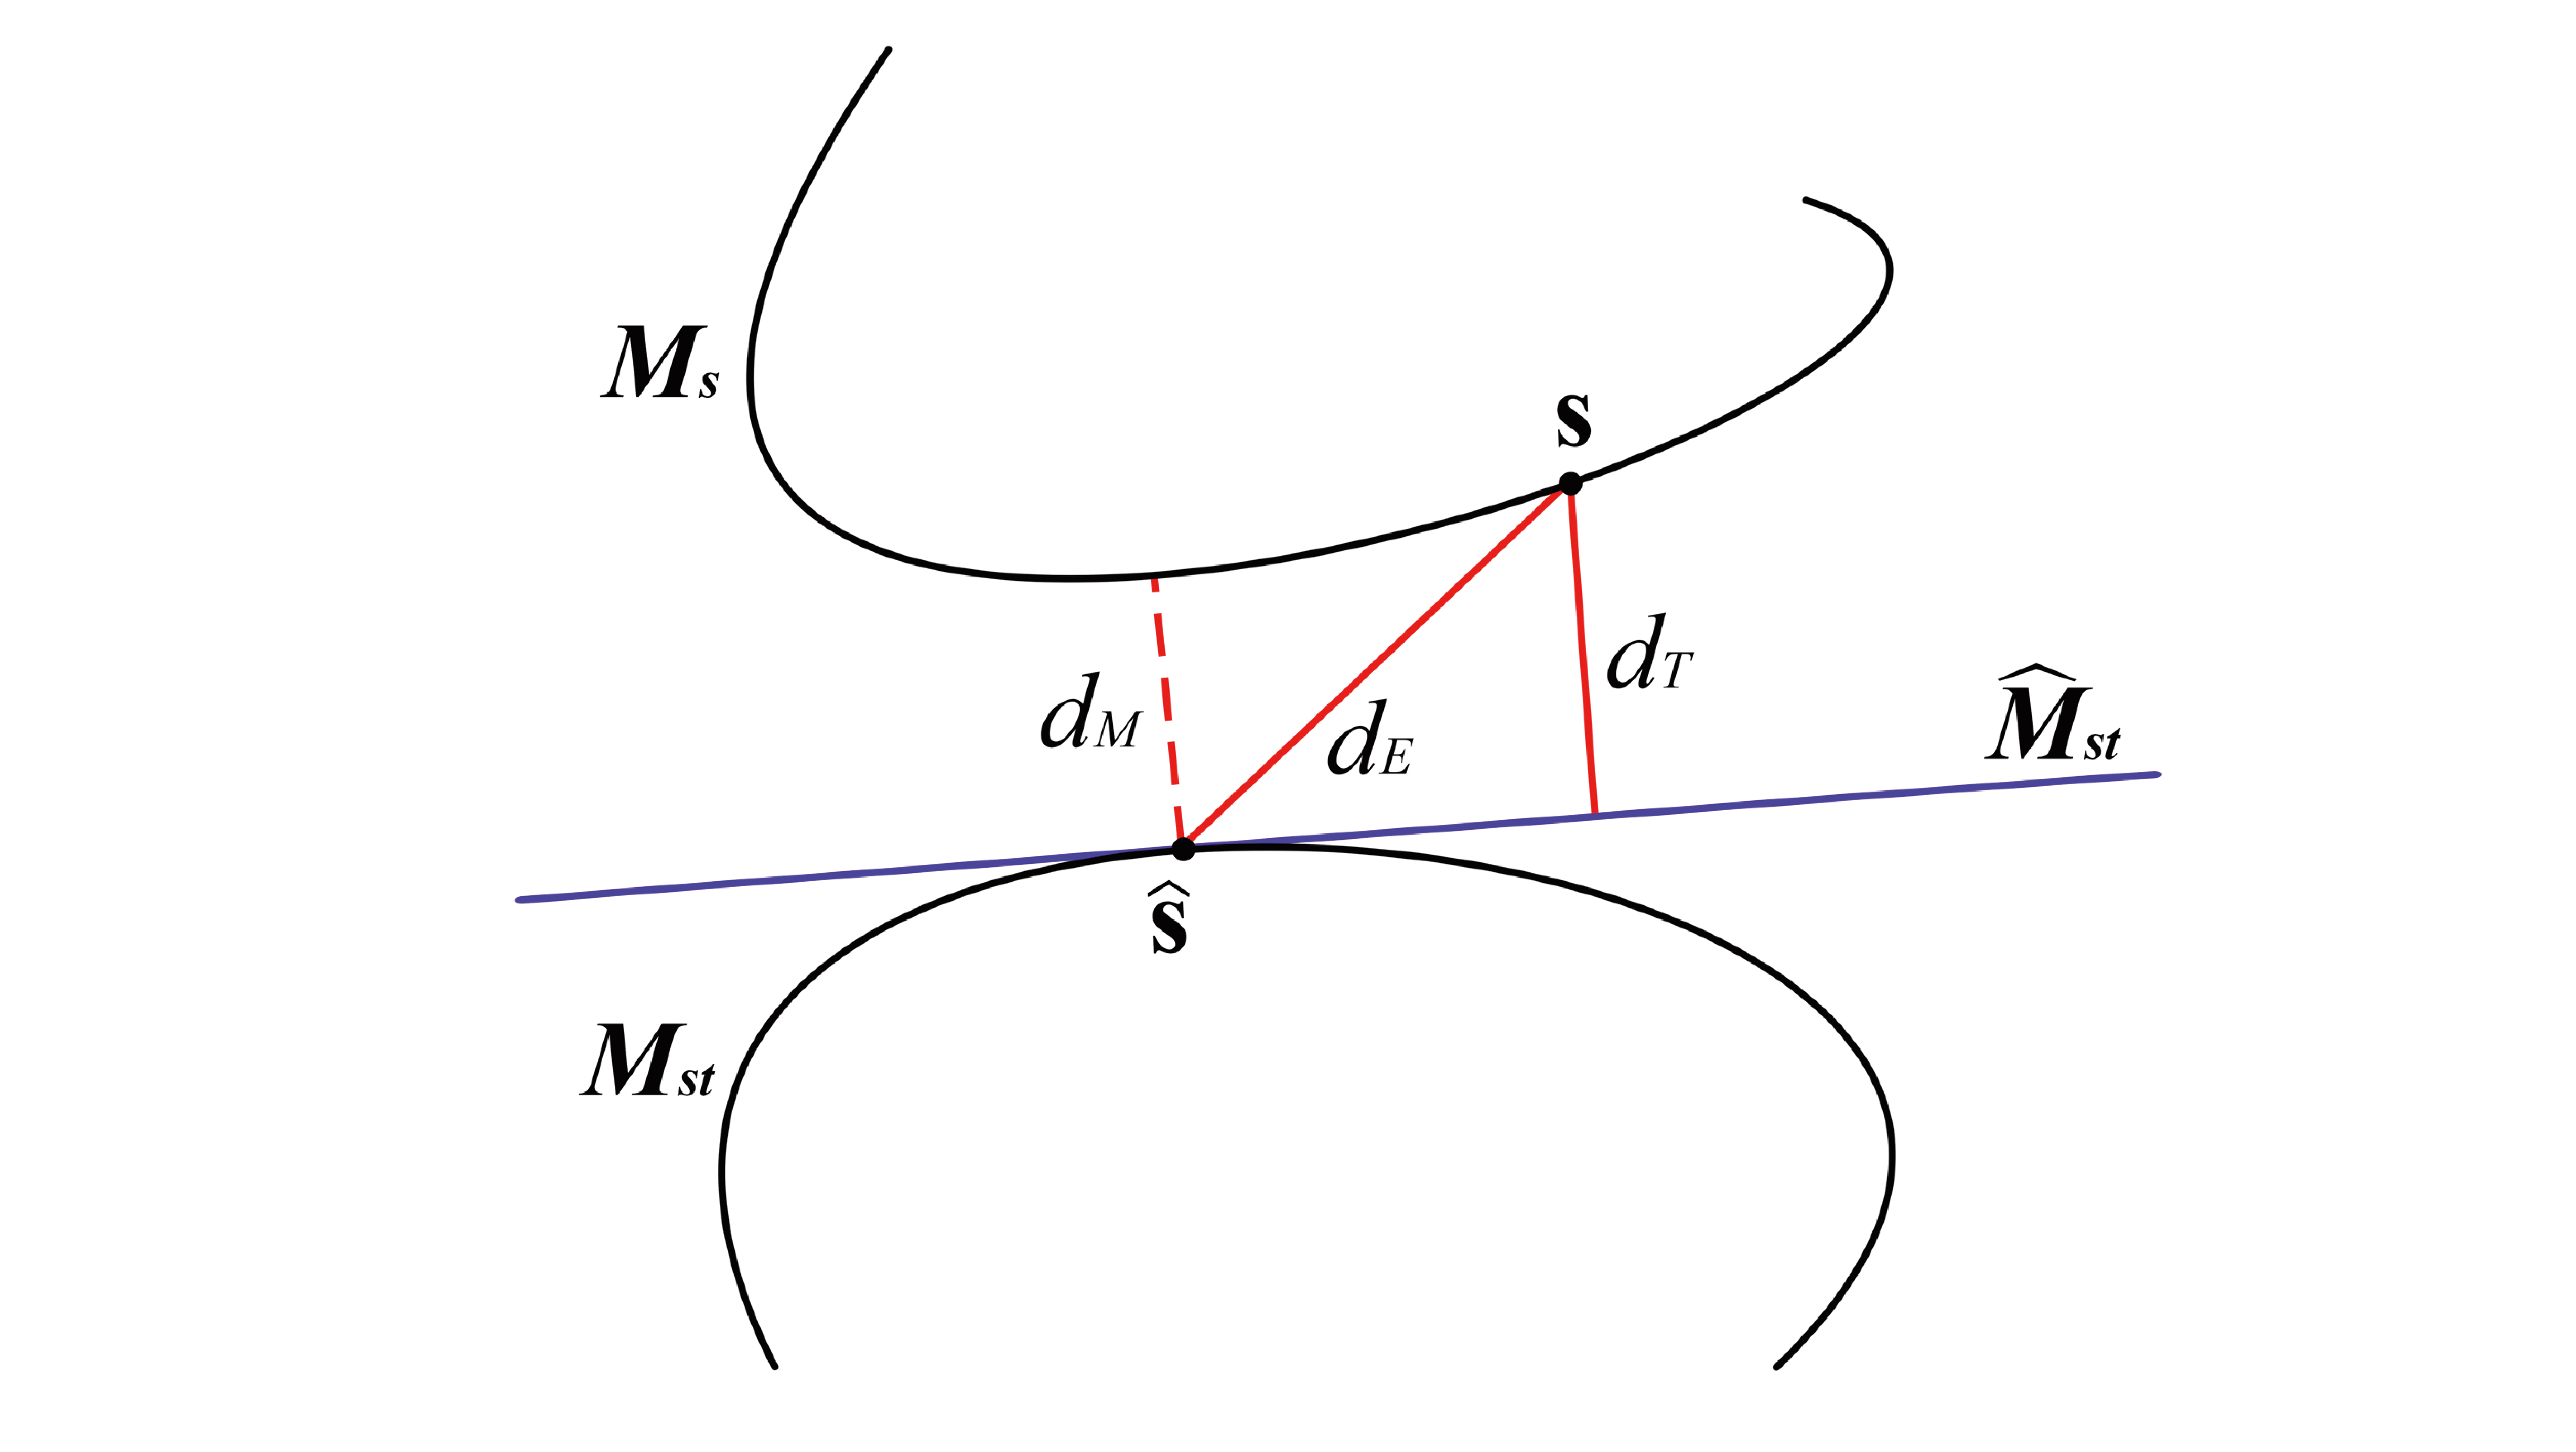
\includegraphics[width=\textwidth]{manifold.pdf}
	\caption{如图展示了欧氏距离、流形间距离和切线距离的关系。在信号空间,$\mathbf{s}$是测试点,$\widehat{\mathbf{s}}$是一个训练点。 $\boldsymbol{M_s}$ 和 $\boldsymbol{M_{st}}$分别是$\mathbf{s}$和$\widehat{\mathbf{s}}$所在的流形。$\boldsymbol{\widehat{M}_{st}}$是$\boldsymbol{M_{st}}$在$\widehat{\mathbf{s}}$处的切线。$d_E$代表$\mathbf{s}$和$\widehat{\mathbf{s}}$之间的欧氏距离。$d_M$代表$\boldsymbol{M_s}$ 和 $\boldsymbol{M_{st}}$两个流形之间的距离。$d_T$代表$\mathbf{s}$到$\boldsymbol{M_{st}}$的切线距离。显然,相比于$d_E$,$d_T$是对$d_M$更好的估计。}
	\label{fig:manifold}
\end{figure}

切线距离是一种对测试点到训练点所在流形距离的局部线性近似,从测试点到训练点流形的切线的距离被称作切线距离,如图\ref{fig:manifold}中$d_T$所示。计算切线距离只需要知道$(\widehat{\mathbf{x}}, \widehat{\mathbf{s}})$处的梯度而不是整个流形,因此切线距离的计算所需数据远小于计算流形之间的距离。

理论上,切线的方向与流形的梯度相同。但是由于不知道流形的具体函数从而很难计算梯度,我们将用有限差分获得切线方向。注意到,在我们的场景中,信号空间内的流形由物理空间的微小变化形成,也就是距离的微小变化。比如,如果$(\mathbf{x}, \mathbf{s})$是一个物理-信号空间对,在物理空间中点$\mathbf{x} + a{\bm{\delta}}$在信号空间内的流形 $\boldsymbol{M_s}$上所对应的点应当表示为 $\boldsymbol{M_s}(a)$。$\delta$是一个表征微小变化方向的单位向量,$a$是一个代表由于物理空间变化导致的距离上变化的标量。这种对距离求导数而不是对物理空间坐标求导数的做法看起来并不直接,因为后者的做法更直观且符合常理。原因是物理坐标$\mathbf{x}$是一个二维或者三维向量,意味着求导需要求偏导数。首先,计算偏导数需要更多的计算及时间。更严重的是,用有限差分法估计偏导数需要$\mathbf{x}$中依次只有一个元素微小变化,其他维度的元素不变,而这对于数据采集是一个严峻挑战,尤其是对于大规模室外数据采集。实际上,如果数据采集条件允许,偏导数或者导数对于后续的分析来说没有区别,除了优化变量从标量变成向量了。总之,偏导数依然适用于切线距离。

\subsection{欧式切线距离}

切线距离起初被提出时就是基于欧氏距离~\cite{simard1998transformation},由下式定义:
\begin{equation}
d_T = \mathop {\min }\limits_{a} {{\left\| \mathbf{s} - \mathbf{t}a - \widehat{\mathbf{s}} \right\|}_2}, \label{eq:euctd}
\end{equation}
其中$\mathbf{s}$和$\widehat{\mathbf{s}}$分别是信号空间中的测试点和训练点。$\mathbf{t}$是训练点附近的导数:
\begin{equation}
\mathbf{t} = {\left( \frac{\partial s_1}{\partial d}, ..., \frac{\partial s_D}{\partial d} \right)}^T, i = 1, 2, ..., D,
\end{equation}
其中$d$代表距离。因为导数是由有限差分近似估计的,在训练集中选择另一个点与训练点进行差分运算就变得至关重要。我们的方法是在物理空间中找到距离训练点最近的$N$个近邻,之后$N$个导数可如下计算:
\begin{equation}
\mathbf{t}_j = \frac{\mathbf{s} - \mathbf{s}_j}{d_j}, j = 1, 2, ..., N.
\end{equation}
注意到$\mathbf{t}_j$代表第$j$个导数而不是向量$\mathbf{t}$的第$j$个元素。$d_j$的距离度量方式无关紧要,因为它只会影响导数的尺度而不是方向,而尺度的影响在\eqref{eq:euctd}中优化$a$时会被消除。关于$N$对于定位精度影响的数值实验将在第\ref{sec:exp}节中被分析。

$d_T$可以通过求解一个线性最小二乘法而简单的获得:
\begin{equation}
a_j = {\left( {\mathbf{t}_j}^T\mathbf{t}_j \right)}^{-1}{\mathbf{t}_j}^T\left( {\mathbf{s}} - \widehat{\mathbf{s}} \right), j = 1, 2, ..., N. \label{eq:euca}
\end{equation}
在所有$a_j$都被计算之后,对于根据\eqref{eq:euctd}得到的所有切线距离$d_{Tj}$求均值,而这将被当做指纹定位中KNN的距离度量方式。

我们将上述距离称为欧式切线距离(Euclidean Tangent Distance, ETD)。虽然ETD很容易求解,但是数值实验显示曼哈顿距离的定位精度优于前文所提到的所有常见距离度量方式,甚至比ETD效果还好。因为ETD的定位精度高于欧氏距离,也许我们可以推演说基于曼哈顿距离的切线距离会比曼哈顿距离表现更好。因此,下一节我们将提出曼哈顿切线距离。

\subsection{曼哈顿切线距离}

为了表述简洁,在后续部分中,导数$\mathbf{t}$和曼哈顿切线距离$d_{MT}$将不会在右下标标注$j$。类似于\eqref{eq:euctd},曼哈顿切线距离可由下式定义:
\begin{equation}
d_{MT} = \mathop {\min }\limits_{a} {\left\| \mathbf{s} - \mathbf{t}a - \widehat{\mathbf{s}} \right\|}_1. \label{eq:mantd}
\end{equation}
但是对$a$优化并不像\eqref{eq:euctd}那么简单,因为L1-范数的导数是符号函数。不妨定义$\mathcal{L} = {\left\| \mathbf{s} - \mathbf{t}a - \widehat{\mathbf{s}} \right\|}_1$,则
\begin{equation}
\frac{\partial \mathcal{L}}{\partial a} = -\mathbf{t}^T \mathrm{sgn}\left( \mathbf{s} - \mathbf{t}a - \widehat{\mathbf{s}} \right). \label{eq:sgn}
\end{equation}
求解\eqref{eq:sgn}是困难的而且甚至无解。在这种情况下,我们需要一种近似函数来尽可能拟合$\mathrm{sgn}(x)$。我们注意到,若双曲正切函数$\mathrm{tanh}(\beta x)$中$\beta \rightarrow \infty$,则$\mathrm{tanh}(\beta x) = \mathrm{sgn}(x)$。因此,我们将用$\mathrm{tanh}(\beta x)$ 代替 $\mathrm{sgn}(x)$,实验中计算时$\beta$取10,000。

令$\mathbf{h} = \mathbf{s} - \mathbf{t}a - \widehat{\mathbf{s}}$,则
\begin{equation}
\frac{\partial \mathcal{L}}{\partial a} = -\mathbf{t}^T \mathrm{tanh}\left( \beta \mathbf{h} \right), \label{eq:deri}
\end{equation}

\begin{equation}
\frac{{\partial}^2 \mathcal{L}}{\partial a^2} = \beta \left( \mathbf{t} \odot \mathbf{t} \right )^T \left[ \mathbf{1} - \mathrm{tanh}\left( \beta \mathbf{h} \right) \odot \mathrm{tanh}\left( \beta \mathbf{h} \right) \right], \label{hessian}
\end{equation}
其中$\odot$是哈达玛积(Hadamard Product),即两个大小相同的矩阵中对应元素相乘,$\mathbf{1}$是全1向量。因为$\mathcal{L}$对$a$求导的导数已经从\eqref{eq:sgn}变为\eqref{eq:deri}了,意味着原函数也从${\left\| \mathbf{h} \right\|}_1$变成$\frac{1}{\beta}\mathbf{1}^T\mathrm{ln}\left[ \mathrm{cosh} \left( \beta \mathbf{h} \right) \right] + C$了,其中$C$是一个常数,这里为了逼近${\left\| \mathbf{h} \right\|}_1$,我们取$C=\mathrm{ln}2$。这两个原函数的对比如图\ref{fig:sgnVSnew}所示,当$|x|>0.0002$时,二者已经几乎完全重合。因此,如果我们用双曲正切函数代替符号函数优化所得的$a$也应当与最优解很接近。在替换后,问题依然是一个凸优化问题(可以很容易证明 $\frac{{\partial}^2 \mathcal{L}}{\partial a^2} > 0$)。虽然如此,曼哈顿距离仍然会被当做目标函数,因为两个原函数差距甚小而且曼哈顿距离容易计算。

如果$\mathbf{t}$是偏导数,$a$将变为一个与物理空间维度相同的向量,相应的一阶导数变成梯度,二阶导数变为海森矩阵。不过这样该问题依然是凸优化问题,因此不影响求解。

\begin{figure}
	\centering
	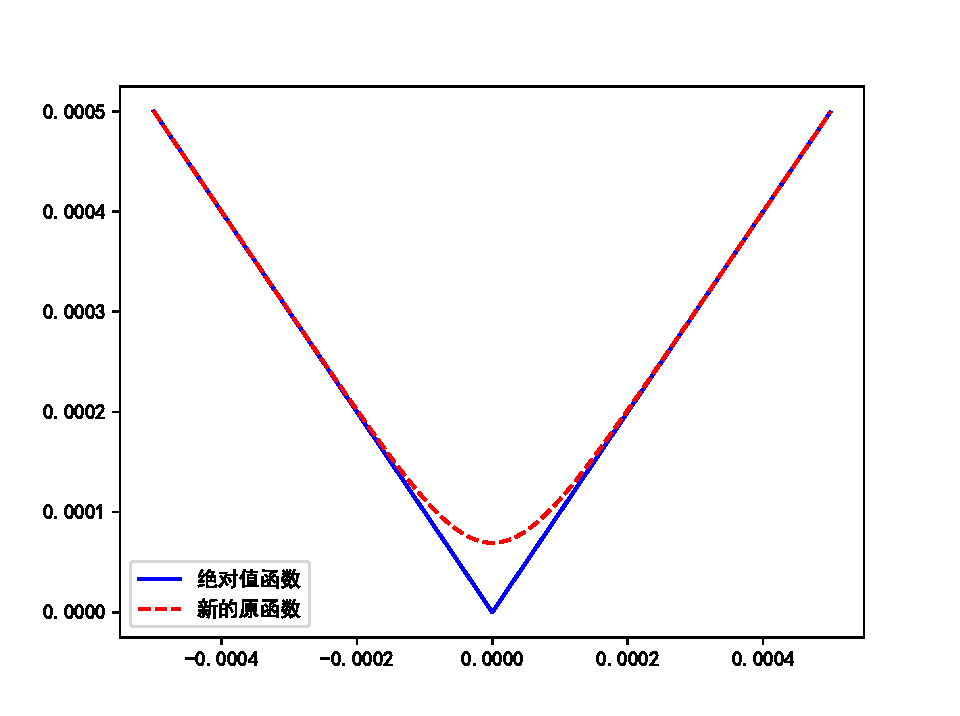
\includegraphics[width=\textwidth]{sgnVSnew.pdf}
	\caption{如图对比了${\left\| x \right\|}_1$和$\frac{1}{\beta}\mathbf{1}^T\mathrm{ln}\left[ \mathrm{cosh} \left( \beta x \right) \right] + \mathrm{ln}2$两种函数的差异,其中$\beta=10,000$。蓝色实线代表曼哈顿距离所基于的绝对值函数,红色虚线代表双曲正切函数的原函数。从图中可以看到,当$|x|>0.0002$时,二者已经几乎完全重合。}
	\label{fig:sgnVSnew}
\end{figure}

既然一阶导数和二阶导数已经由\eqref{eq:deri}和\eqref{eq:hessian}给出,$\mathcal{L}$可由牛顿法(Newton's Method)求解从而得到曼哈顿切线距离。我们把这个距离度量方式称为曼哈顿切线距离(Manhattan Tangent Distance, MTD)。它的物理意义是对测试点和训练点所在的流形之间的曼哈顿距离的局部线性近似,也就是在切线上找到一点使得它到测试点的距离最小。

\subsection{低计算复杂度的近似解法}

虽然在上一节中我们提出了一种求解MTD的方法,但是该方法的缺点也是很明显的:过高的计算复杂度。该方法的时间复杂度是曼哈顿距离的$\mathcal{O}(NS)$倍,其中$N$是用有限差分法计算梯度所需的近邻数,$S$是牛顿法收敛所需的迭代步数。因为每次计算曼哈顿切线距离都需要迭代求解一个凸优化问题,若在线上系统中采用可能会有过高延迟。

因为切线距离是对物理空间中$\mathbf{x}$附近的点在信号空间中所形成的流形的局部线性近似,即\eqref{eq:mantd}中的切线距离只有在$a$接近0时才是对流形较好的估计。此外,我们注意到双曲正切函数$\mathrm{tanh}(x)$的一阶泰勒近似可写为$\mathrm{tanh}(x) = x + \mathcal{O}\left( x^3 \right)$。如果我们用$\mathrm{tanh}(x)$的一阶泰勒级数$x$代替它,则\eqref{eq:deri}中的$\frac{\partial \mathcal{L}}{\partial a}$将变为
\begin{equation}
\frac{\partial \mathcal{L}}{\partial a} = -\beta \mathbf{t}^T \left( \mathbf{s} - \mathbf{t}a - \widehat{\mathbf{s}} \right). \label{eq:approx}
\end{equation}
令\eqref{eq:approx}等于0的解和\eqref{eq:euca}一样。换句话说,近似算法中$a$的求解将采用和欧式切线距离相同的方法,但是将$a$带回目标函数计算切线距离时是基于曼哈顿距离的。我们把该算法叫做近似曼哈顿切线距离(Approximate Manhattan Tangent Distance, AMTD)。

AMTD的时间复杂度是简单曼哈顿距离的$\mathcal{O}(N)$倍,相比于MTD,复杂度降低了$S$倍。

\section{实验与结果} \label{sec:exp}

\subsection{数据采集与预处理}

\begin{figure}
	\centering
	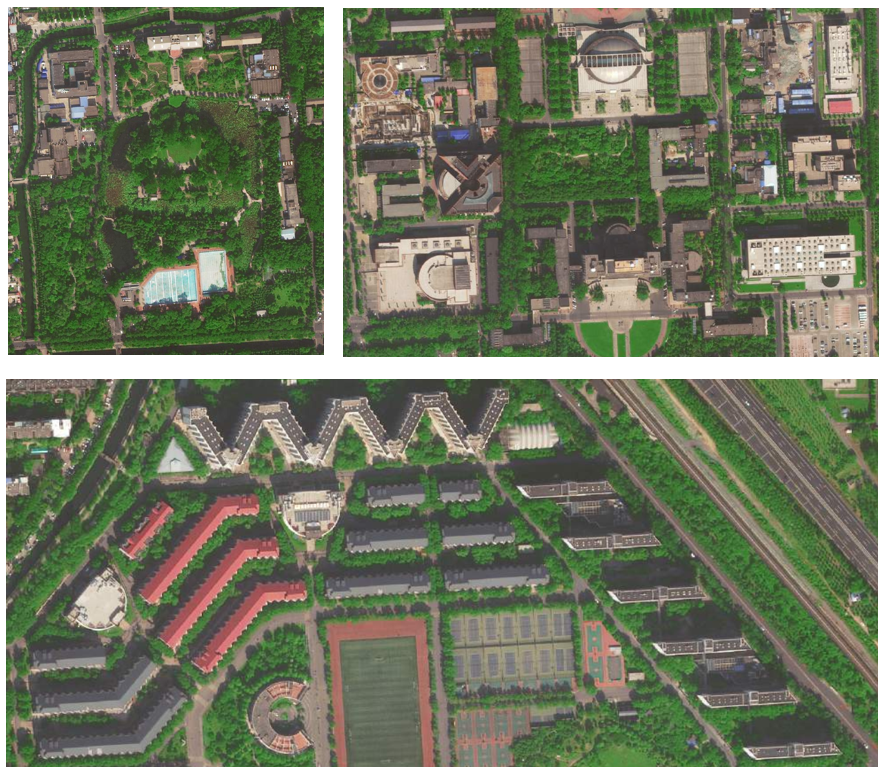
\includegraphics[width=\textwidth]{data_collection_area.png}
	\caption{如图所示为我们采集数据的三个区域的卫星图。左上子图为荷塘区域,右上子图为教学区,下子图为紫荆公寓区。}
	\label{fig:data_collection}
\end{figure}

这一节所用的数据由我们自己利用路测仪在清华大学校园内采集所得,路测仪在收集附近所有可接收信号基站的RSS的同时,还会收集GPS的定位信息。我们分别在三个不同的区域采集数据:
\begin{enumerate}
	\item 荷塘。这里是一个池塘,池塘中间有一个湖心岛,有很多树木但是没有高层建筑,如图\eqref{fig:data_collection}左上子图所示。这片区域总面积是$0.097\mathrm{km}^2$。数据由实验员手持路测仪步行采集,数据采集频率0.2Hz,两个时序相邻点的平均距离是5.0m。该数据集共有621个样本和85个可探测基站;
	\item 教学区。这片区域有一些高层建筑和树木,但是道路宽敞而且楼间距宽,如图\eqref{fig:data_collection}右上子图所示。这片区域总面积是$0.416\mathrm{km}^2$。数据由实验员骑车采集,路测仪采样频率0.5Hz。两个时序相邻点的平均距离是4.8m。该数据集共有2273个样本和204个可探测基站;
	\item 紫荆公寓区。这片区域有很多中层建筑而且道路狭窄,如图\eqref{fig:data_collection}下子图所示。这片区域总面积为$0.143\mathrm{km}^2$。数据由实验员骑车采集,路测仪采样频率0.5Hz。两个时序相邻点的平均距离是4.4m。该数据集共有1035个样本和149个可探测基站。
\end{enumerate}

虽然数据集中有很多可探测基站,但是对于每一条采样的接收信号来说,不会所有基站都有RSS,即数据会存在某些基站无接收信号的情况。为了应对这个问题,我们把每个基站的最小RSS减1作为缺省值。

\subsection{指数变换参数$\lambda$的选择} \label{subsec:lambda}

\begin{figure}
\centering
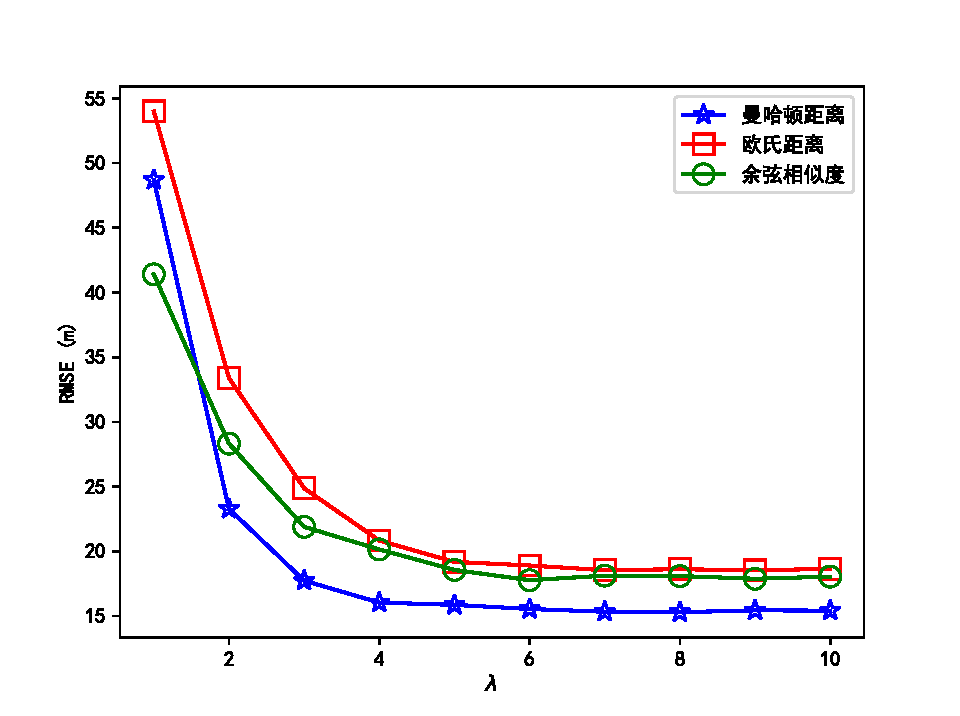
\includegraphics[width=\textwidth]{RMSE_lam.pdf}
\caption{如图所示为指数变换中参数$\lambda$与定位均方根误差RMSE的关系曲线,蓝色星形线是曼哈顿距离,红色方形线是余弦相似度,绿色圆形线是欧氏距离。当$\lambda>7$后RMSE几乎没有明显变化。}
\label{fig:rmse_lam}
\end{figure}

\begin{table}[tbp]
	\caption{指数变换后RMSE比较}
	\begin{center}
		\begin{tabular}{ccc}
			\toprule
			\textbf{RMSE/m} & \textbf{无指数变换} & \textbf{指数变换 ($\lambda=10$)} \\
			\midrule
			\textbf{曼哈顿距离} & 15.85 & 15.41 \\
			\midrule
			\textbf{欧氏距离} & 20.97 & 18.65 \\
			\midrule
			\textbf{余弦相似度} & 20.28 & 18.04 \\
			\bottomrule
		\end{tabular}
		\label{tab:no_exp}
	\end{center}
\end{table}

为了使定位效果最优,我们开展实验以找到指数变换中最优的$\lambda$参数,实验中KNN的参数k=3。对于不同的三种常用距离度量方式,画出$\lambda$与RMSE之间的关系曲线,如图\ref{fig:rmse_lam}所示。这里只有从荷塘采集的数据参与了实验,一是为了减少计算时间,二是防止过拟合,即后两个数据集没有参与参数$\lambda$的调节,而是直接使用。为了尽可能消除噪声的影响并使曲线平滑,对于每个$\lambda$均随机选取10\%的数据作为测试数据并随机进行1000次。从图中可以看出当$\lambda>7$后RMSE几乎没有明显变化,因此在后续实验中我们将令$\lambda=10$。

作为对比,不采用指数变换的指纹定位效果在表\ref{tab:no_exp}中给出,其中指数变换的$\lambda=10$。实验结果显示指数变换的确可以一定程度上提高定位精度。

此外,很明显曼哈顿距离可以取得最小的定位误差,因此在我们的数据集下,最常用的欧氏距离并不是最优选择。至于余弦相似度,它的表现比欧氏距离好,但是依然劣于曼哈顿距离。

\subsection{KNN中近邻数k的选择}

\begin{figure}
	\centering
	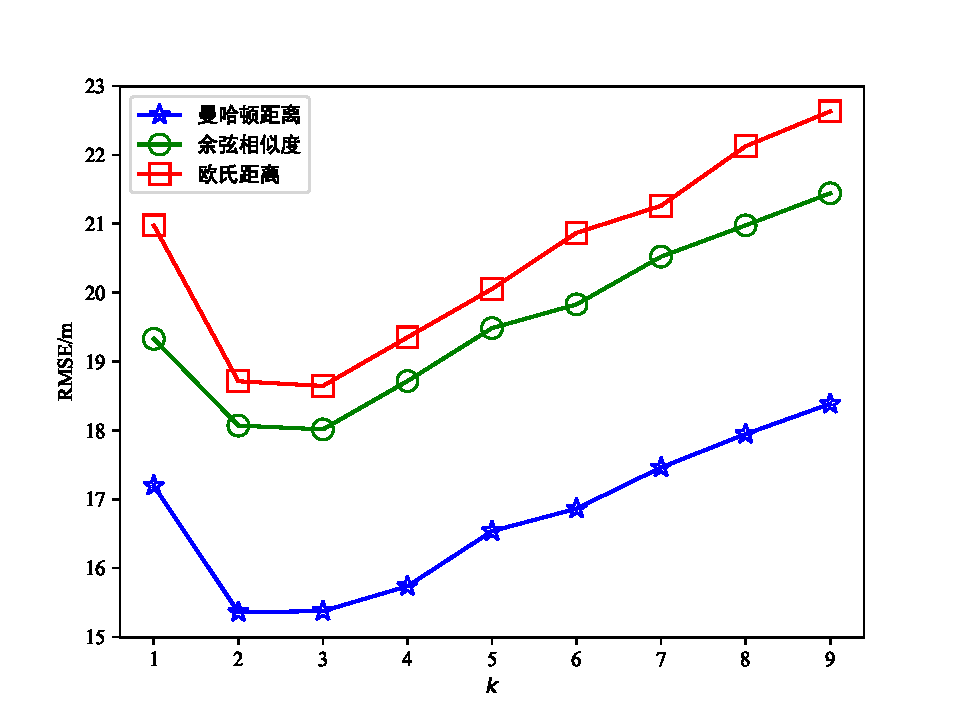
\includegraphics[width=\textwidth]{RMSE_k.pdf}
	\caption{如图所示为KNN中参数$k$与定位均方根误差RMSE的关系曲线,蓝色星形线是曼哈顿距离,绿色圆形线是余弦相似度,红色方形线是欧氏距离。当$k$取2或3时可以取得最小定位误差。}
	\label{fig:rmse_k}
\end{figure}

此处仍然只使用荷塘的数据。在$\lambda=10$的条件下,针对不同的参数$k$开展实验,测试集的选取和实验次数与第\ref{subsec:lambda}节的设置相同。实验结果如图\ref{fig:rmse_k}所示。对于三种度量方式来说,都是在$k$=2或3时RMSE最小,因此在后续的实验中我们将把$k$固定为3。

\subsection{切线距离的导数中参数$N$的选择}

\begin{figure}
	\centering
	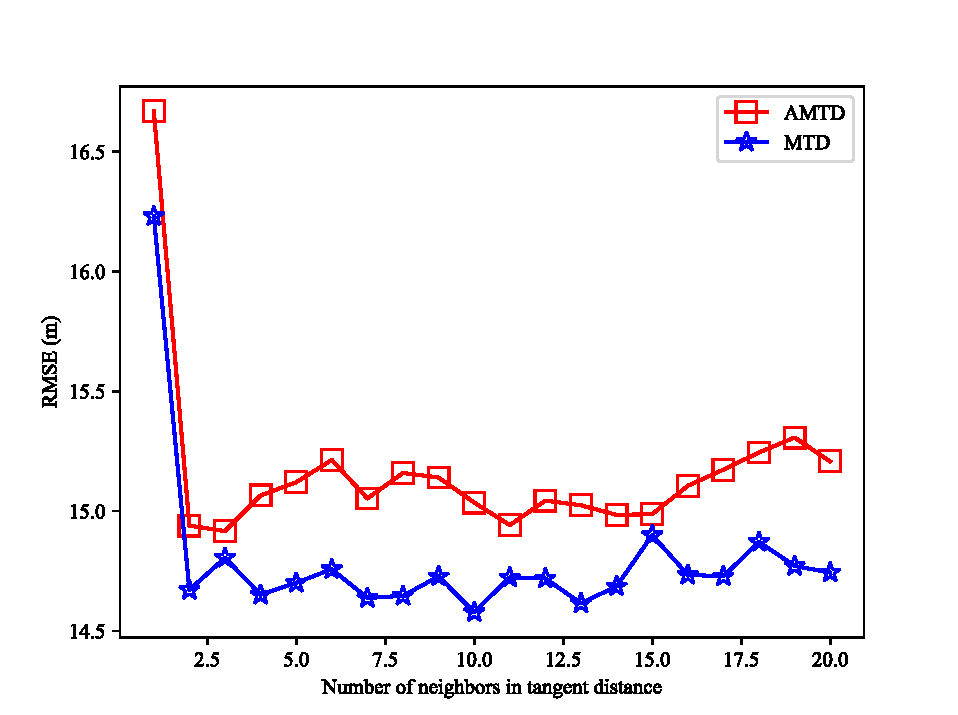
\includegraphics[width=\textwidth]{RMSE_N.pdf}
	\caption{如图所示为求解切线距离时求导数所需近邻数$N$与定位均方根误差RMSE的关系曲线,蓝色星形线是曼哈顿切线距离MTD,红色方形线是近似曼哈顿切线距离AMTD。由于实验次数少导致曲线波动较大,不过大致可以看出当$N>2$时几乎没有太大的变化。}
	\label{fig:rmse_n}
\end{figure}

这里依然只使用荷塘的数据。这里使用K-fold方法,即将数据集随机分成k份,之后循环k次,依次取一份作为测试数据,其余k-1份作为训练数据。在该实验中k=10即每次取10\%的数据作为测试数据。每个fold中,MTD和AMTD将同时训练和测试。在MTD中,牛顿法的停止判据是$10^{-4}$。

图\ref{fig:rmse_n}是实验结果。虽然由于实验次数少导致曲线一直在抖动,但是总体趋势大致是先急剧下降,在$2 \le N \le 15$的范围内基本不变,之后缓慢上升。在综合考虑精度和计算复杂度后,我们决定在后续实验中将$N$设为5。

\subsection{切线距离定位效果}

\begin{table}[tbp]
	\caption{切线距离定位效果对比}
	\begin{center}
		\begin{tabular}{cccc}
			\toprule
			RMSE/m &  荷塘 & 教学区 & 公寓区 \\
			\midrule
			欧氏距离 & 19.20 & 13.56 & 10.29 \\
			\midrule
			ETD & 16.69 & 11.47 & 9.54 \\
			\midrule
			曼哈顿距离 & 15.78 & 9.96 & 7.95 \\
			\midrule
			\textbf{MTD} & \textbf{14.75} & \textbf{9.14} & \textbf{7.45} \\
			\midrule
			\textbf{AMTD} & \textbf{14.90} & \textbf{9.43} & \textbf{7.63} \\
			\bottomrule
		\end{tabular}
		\label{tab:td}
	\end{center}
\end{table}

\begin{table}[tbp]
	\caption{切线距离定位效果对比}
	\begin{center}
		\begin{tabular}{cccc}
			\toprule
			RMSE相对减少 &  荷塘 & 教学区 & 公寓区 \\
			\midrule
			MTD & -6.53\% & -8.23\% & -6.29\% \\
			\midrule
			AMTD & -5.58\% & -5.32\% & -4.03\% \\
			\bottomrule
		\end{tabular}
		\label{tab:td_relative}
	\end{center}
\end{table}

综合上述实验的结论,我们令指数变换参数$\lambda=10$,KNN中的参数$k=3$。涉及切线距离时,计算导数所需的近邻数$N$设为5。本小节中我们将比较欧式距离、欧式切线距离、曼哈顿距离、曼哈顿切线距离和近似曼哈顿切线距离的定位效果。

实验结果展示在表\ref{tab:td}中。首先,注意到欧式切线距离ETD可以取得比欧氏距离更小的RMSE,但是仍然高于简单的曼哈顿距离,这也是我们提出曼哈顿切线距离MTD的动机。其次,实验结果显示MTD在所有三个数据集中均取得最小的RMSE。除此之外,虽然近似曼哈顿切线距离AMTD的RMSE略高于MTD,但是仍然低于曼哈顿距离的RMSE而且在我们的实验中效果仅次于MTD,而且计算复杂度远小于MTD。相比于曼哈顿距离,在三个数据集中,MTD和AMTD相比于曼哈顿距离的相对RMSE减少如表\ref{tab:td_relative}所示。显然,无论对于MTD还是AMTD来说,从公寓区采集的数据定位精度提升的最小。我们分析可能的原因是公寓区采集的数据其时序相邻点的平均距离最小,因此相比于其他数据集,像曼哈顿距离等简单距离度量方式能够更好的估计流形之间的距离。但是定位精度受到很多其他因素影响,比如信道信息等。相比于其他区域,公寓区的建筑较高而且密集,这可能导致距离的小幅变化反映到信号空间会变化较大,这也会限制MTD和AMTD的提升效果。

\section{本章小结}

这一章我们讨论了将切线距离应用于基于接收信号强度和加权-KNN的指纹定位算法中。首先,我们简单介绍了指纹定位的KNN算法中常见的距离度量方式,并分析了他们的缺点,包括给予不同大小的RSS相同的权重以及在流形存在的情况下简单度量方式不能反映真实距离等问题。针对这些问题,我们分别利用指数变换和切线距离来解决。其后,我们阐明了切线距离背后所蕴含的思想,并介绍了原作者所提出的基于欧氏距离的切线距离ETD。然而,因为在实测数据实验中欧式切线距离的定位效果虽然相较于欧氏距离有提升,但是依然劣于曼哈顿距离,于是我们提出了曼哈顿切线距离MTD以及在定位精度和计算复杂度之间折中的近似曼哈顿切线距离AMTD。为了验证算法性能,我们在清华大学校园内不同的三个区域采集数据,开展实验找到适合的KNN近邻数$k$、指数变换参数$\lambda$以及切线距离中计算导数所需的近邻数$N$。最后,我们比较了欧氏距离、ETD、曼哈顿距离、MTD和AMTD的定位误差RMSE。在所有三个数据集中,MTD均取得了最小的定位误差,而AMTD则以远小于MTD的计算量取得了仅次于MTD却依然优于曼哈顿距离的定位精度。






\chapter{保量推荐下的最优广告投放算法}
\label{cha:allocation}

本章我们将提出一种\textit{最优广告投放算法(oPtImal Kwai Advertising, PIKA)},该算法被部署在快手广告平台中的同城页粉丝头条服务中。粉丝头条服务致力于在保证广告主获得其期望的曝光量的情况下,使得广告投放后的总分数最高,其中分数由\ref{eq:score}定义。长达一个月的线上实验表明PIKA的广告投放效果优于目前部署在线上的算法。PIKA算法的核心思想是利用坐标下降法求解一个离线的带约束二次规划问题的KKT条件,该算法分为两个部分:训练模块和投放模块,分别对应线下部分和线上部分。不同于之前所部署的流量控制算法中的硬阈值,PIKA中线下优化所得的对偶变量可以被认为是一种“软阈值”,而算法会根据不同广告的需求投放量和历史数据中的分数给其设置不同的软阈值,进而在满足投放量的同时最大化投放后的总分数。

\section{PIKA算法原理}

\subsection{问题定义}

不妨设$\mathcal{S}$是所有在投广告的集合,它的一个子集$\mathcal{S}_i$第$i$次PV所召回的广告集合,则$\mathcal{S}_i \subset \mathcal{S}$。每个在投广告的总期望曝光量或者说总需求量用$D_j$表示,该广告的投放时长用$T_j$表示。理想情况下,我们希望在投放时长到达$T_j$后,最终的实际广告投放量正好等于$D_j$,因此实际中我们尽量使最终曝光量尽可能接近$D_j$。除此之外,每次PV对于被召回广告的分数也将被用于目标函数。因为对于每次PV只有一小部分广告被召回,因此我们可以用一个稀疏矩阵$\bm{A}$来存储PV对广告的分数,其中$\bm{A}_{ij}$是预测出的第$i$次PV对于第$j$个广告的分数。因此,如果一段时间内有$M$次访问和$N$个在投广告,那么$\bm{A}$应当是一个$M \times N$的矩阵。如果对于第$i$次PV来说,广告$j$没有被召回,则$\bm{A}_{ij}=0$。

最后却也是最重要的,投放矩阵$\bm{X}^{int}$决定每次PV投放哪个广告,即若 $\bm{X}^{int}_{ij} = 1$则将广告$j$投放给PV $i$,否则$\bm{X}^{int}_{ij} = 0$。这是一个\textit{0-1整数规划问题(0-1 Integer Programming Problem)},而且该问题是一个NP-complete问题~\cite{garey2002computers}。为了克服这个困难,我们将投放矩阵松弛为投放概率矩阵$\bm{X}$,它拥有和$\bm{A}$相同的大小,其中$\bm{X}_{ij}$代表将广告$j$投放给PV $i$的概率。为了防止用户体验被广告过多影响,我们要求每次PV只能投放少量广告。如果每次PV最多只能投放1个广告,则
\begin{equation}
\sum_j \bm{X}_{ij} \le 1, \forall i.
\end{equation}
这个约束与概率的归一性(即随机变量所有可能取值的概率之和或概率密度积分等于1)一致,因为不投放广告的概率没有被纳入$\bm{X}$中,而对于PV $i$不投放广告的概率就是$1-\sum_j \bm{X}_{ij}$。每次PV可以投放多个广告的场景将在第\ref{subsec:more_than_one}节中讨论。此外,因为概率的非负性,我们有$\bm{X}_{ij} \ge 0, \forall i,j$。在常见的广告投放算法中,平台从广告主得到的收入小于等于广告日的每日预算是合理的。但是,为了在收入和用户体验之间取得平衡,这里我们将采用等式约束来使广告的最终曝光量等于广告主的需求量。

最后,我们正式用如下优化表达式描述我们的问题:
\begin{equation}
\begin{aligned}
\min_X &-\sum_{i,j} \bm{A}_{ij}\bm{X}_{ij} \\
s.t. & \sum_i \bm{X}_{ij} = \bm{d}_j, \forall j, \\
& \sum_j \bm{X}_{ij} \le 1, \forall i, \\
& \bm{X}_{ij} \ge 0, \forall i, j. 
\label{eq:ori_opt}
\end{aligned}
\end{equation}
$\sum_{j} \bm{A}_{ij}\bm{X}_{ij}$是PV $i$的分数的期望,因此目标函数$\sum_{i,j} \bm{A}_{ij}\bm{X}_{ij}$的含义就是所有PV的期望分数的总分数。为了与优化问题的标准格式一致,我们最小化目标函数的负值,而且由于它是一个线性函数,因此正负号不影响凹凸性。注意到,上式中的需求量符号是$\bm{d}_j$而不是$D_j$,这里$\bm{d}_j$代表训练周期内的期望需求量。作为一个简单的例子,对于广告$j$来说,如果当前客户端展示量,或者说曝光量,是$\bm{c}_j$,剩余投放时长是$\bm{t}_j$,训练周期是$T_p$(即每隔$T_p$求解一次上述优化问题),则$\bm{d}_j$可以用如下公式计算:
\begin{equation}
\bm{d}_j = \frac{D_j - \bm{c}_j}{\bm{t}_j}T_{p}. \label{eq:avg}
\end{equation}
平滑投放通过上式里把总需求量均匀分散于投放时长内的所有训练周期被隐式的实现了,不过真实环境中流量是有高峰和低谷的,一个线上可用的需求量分配方案将在第\ref{subsec:hourly_d}节中被详细介绍。

这是一个标准的带约束的\textit{线性规划问题(Linear Programming problem, LP)},而且已经有很多成熟的解法。但是,简单的给出最优解$\bm{X}$并不适用于我们的场景,因为我们所需要的是一个等式来指导线上广告投放,从而当被召回广告及其分数可用时我们可以迅速给出投放概率。而如果只是简单的算出最优$\bm{X}$,这也只是历史数据的最优解,无法用于未来PV的广告投放。通过在目标函数里加入$\bm{X}$的二次项可以得到关于$\bm{X}$和对偶变量的等式。此外,由于噪声的存在以及预测分数$\bm{A}$的抖动,如果直接优化$\sum_{i,j} \bm{A}_{ij}\bm{X}_{ij}$可能会导致过拟合和求解结果不稳定。另一个出发点是,$\bm{X}$中的非零值元素比较分散的情况应该好于非零值集中在少数几个元素,因为前者对于分数$\bm{A}$的变化不敏感。因此,我们在\eqref{eq:ori_opt}的基础上加入正则项:
\begin{equation}
\begin{aligned}
\min_X &\sum_{i,j}  (-\bm{A}_{ij}\bm{X}_{ij} + \frac{\lambda}{2}{\bm{X}_{ij}}^2) \\
s.t. & \sum_i \bm{X}_{ij} = \bm{d}_j, \forall j, \\
& \sum_j \bm{X}_{ij} \le 1, \forall i, \\
& \bm{X}_{ij} \ge 0, \forall i, j, 
\label{eq:opt}
\end{aligned}
\end{equation}
其中$\lambda$是正则化系数。

\eqref{eq:opt}将在线下求解之后用于指导线上投放,因此我们的算法可以分为两部分:训练模块和投放模块。

\subsection{训练模块} \label{subsec:train}

在训练之前,服务器会为训练收集历史数据。之后求解优化问题\eqref{eq:opt}。显然,\eqref{eq:opt}是一个凸优化问题,意味着满足KKT条件的解就是优化问题的最优解。对于$\forall i,j$,\eqref{eq:opt}的KKT条件是:
\begin{equation}
\begin{aligned}
\sum_i{\bm{\hat{X}}_{ij}} - \bm{d}_j &= 0, \\
\sum_j{\bm{\hat{X}}_{ij}} -1 &\le 0, \\
\bm{\beta}_i &\ge 0, \\
\bm{\beta}_i\sum_j \bm{\hat{X}}_{ij} &= 0, \\
-\bm{\hat{X}}_{ij} &\le 0, \\
\bm{\Gamma}_{ij} &\ge 0, \\
\bm{\Gamma}_{ij}\bm{\hat{X}}_{ij} &= 0, \\
-\bm{A}_{ij} + \lambda\bm{\hat{X}}_{ij} + \bm{\alpha}_j + \bm{\beta}_i - \bm{\Gamma}_{ij} &= 0, \\ 
\label{eq:kkt}
\end{aligned}
\end{equation}
其中$\bm{\hat{X}}$是理论上的最优解,$\bm{\alpha}, \bm{\beta}$和$\bm{\Gamma}$分别是对应\eqref{eq:opt}中的三个约束的对偶变量。由\eqref{eq:kkt}可以发现$\bm{\hat{X}}_{ij}$ 和 $\bm{\Gamma}_{ij}$二者至少有一个必须等于0,再加上$\bm{X}_{ij} \ge 0$的约束,我们可用下式表示$\bm{\hat{X}}_{ij}$:
\begin{equation}
\bm{\hat{X}}_{ij} = \max\{0, \frac{1}{\lambda} (\bm{A}_{ij} - \bm{\alpha}_j - \bm{\beta}_i)\}, \forall i, j. 
\label{eq:xeq}
\end{equation}
将上式带回\eqref{eq:kkt}中,则可以改写为:
\begin{equation}
\begin{aligned}
\sum_i{\bm{\hat{X}}_{ij}} - \bm{d}_j &= 0, \\
\sum_j{\bm{\hat{X}}_{ij}} - 1 &\le 0, \\
\bm{\beta}_i &\ge 0, \\
\bm{\beta}_i\sum_j \bm{\hat{X}}_{ij} &= 0, \\
\bm{\hat{X}}_{ij} - \max\{0, \frac{1}{\lambda} (\bm{A}_{ij} - \bm{\alpha}_j - \bm{\beta}_i)\} &= 0. \\ 
\end{aligned}
\end{equation}
这样就已经减少到2个对偶变量了,而且其中一个还是对应等式约束的对偶变量,即$\bm{\alpha}$。因此,我们可以利用坐标下降法获得最优解,其中$\bm{\alpha}$和$\bm{\beta}$依次被优化并迭代,直到到达停止迭代判据或者迭代次数。因为$\bm{\alpha}$对应等式约束,因此在计算$\bm{\alpha}_j$时可以固定住$\bm{\beta}$,并行的解算,使得 $\sum_i{\bm{\hat{X}}_{ij}} - d_j = 0$。至于计算$\bm{\beta}$,可以先将其全部设为0,如果$\sum_j{\bm{\hat{X}}_{ij}} \le 1$,则继续令$\bm{\beta}_i=0$;否则并行的计算$\bm{\beta}_i$使得$\sum_j{\bm{\hat{X}}_{ij}} = 1$。算法\ref{alg:offline}完整的描述了离线最优解算法。

\begin{algorithm}[tb]
	\caption{离线最优解算法} 
	\label{alg:offline}
	\begin{algorithmic}[1]
		\REQUIRE 分数矩阵 $\bm{A}$, 需求量 $\bm{d}$, 在投广告数 $M$, 上一个周期内的访问数 $N$, 收敛界 $b$
		\ENSURE 对偶变量 $\bm{\alpha}$ 
		\STATE 初始化: $\bm{\beta}_i \leftarrow 0$ for all $i$, $\bm{\alpha}_j \leftarrow 0$, $\bm{\alpha}^{old}_j \leftarrow 1$ for all $j$
		\WHILE{${\left\| \bm{\alpha}^{old} - \bm{\alpha} \right\|}$ > 停止判据 \&\& 迭代步数 < 步数阈值} 
		\FOR{$i < N$}
		\IF{$\sum_j \bm{X}_{ij} \le 1$}
		\STATE $\bm{\beta}_i \leftarrow 0$
		\ELSE
		\STATE 求解 $\bm{\beta}_i$ s.t. $\sum_j \bm{X}_{ij} = 1$ \label{solve_beta}
		\ENDIF
		\ENDFOR
		\FOR{$j < M$}
		\STATE 求解 $\bm{\alpha}_j$ s.t. $\sum_i \bm{X}_{ij} = \bm{d}_j$ \label{solve_alpha}
		\IF{$\bm{\alpha}_j < b$}
		\STATE 广告 $j$ 无解而且不会参与后续迭代的计算 \label{bound}
		\ENDIF
		\ENDFOR
		\STATE $\bm{\alpha}^{old} \leftarrow \bm{\alpha}$
		\ENDWHILE
		\RETURN $\bm{\alpha}$ 
	\end{algorithmic}
\end{algorithm}

算法\ref{alg:offline}中的$\bm{X}_{ij}$均由\eqref{eq:xeq}计算。$\bm{X}$的求和其实是一个分段折线函数,因此我们可以用二分法来实现算法\ref{alg:offline}中的求根操作(第\ref{solve_alpha}行和第\ref{solve_beta}行)。这里的$\bm{\alpha}$可以被认为是一种“软阈值”:当$\bm{A}_{ij} \le \bm{\alpha}_j$时,广告$j$不可能被投放给PV $i$;当$\bm{A}_{ij} > \bm{\alpha}_j$时,$\bm{A}_{ij}$越大则广告$j$被投放给PV $i$的概率越大。因此在某种程度上说,$\bm{\alpha}$揭露了广告$j$的分数和它的需求量之间的某种关系。

然而,简单的交替求解$\bm{\alpha}$和$\bm{\beta}$或者说坐标下降可能会因为一些广告无解的情况存在而整体不收敛。比如,当一个广告在上一个训练周期内的召回量太少甚至少于需求量时,这个广告是无解的。一种可能的解决方案是像SHALE~\cite{bharadwaj2012shale}一样,在我们的优化表达式中加一个惩罚项:
\begin{equation}
\begin{aligned}
\min_X &\sum_{i,j}  (-\bm{A}_{ij}\bm{X}_{ij} + \frac{\lambda}{2}{\bm{X}_{ij}}^2) + \sum_j \bm{p}_j\bm{u}_j  \\
s.t. & \sum_i \bm{X}_{ij} + \bm{u}_j = \bm{d}_j, \forall j, \\
& \sum_j \bm{X}_{ij} \le 1, \forall i, \\
& \bm{X}_{ij} \ge 0, \bm{u}_j \ge 0. \forall i, j. 
\end{aligned}
\end{equation}
但是,这种方法会增加计算复杂度,而且引入了另一个需要调节的超参数$\bm{p}$。因为快手的召回系统机制可以确保没有一个广告会一直召回量不足,因此我们可以简单的放弃在下个周期通过上述正常方式投放该广告。我们设置了一个界限$b$,当迭代过程中$\bm{\alpha}_j$比$b$还小,该广告$j$就会被认为是无解的,并不会参与本周期的后续迭代计算。只设置下界$b$的原因是$\bm{\alpha}$其实存在一个隐式的上界,这个值是一个跟该广告分数和需求量相关的值。而一旦一个广告召回量太少,迭代过程中$\bm{\alpha}_j$就会一直减小,最终触发下界停止迭代。无解的广告无法通过下一小节将要介绍的正常的投放模块投放出去,而这些广告的投放方法将在第\ref{subsec:guarantee}节中讨论。

$\bm{\alpha}$是投放模块唯一需要从训练模块获得的参数,因此训练模块只需返回$\bm{\alpha}$即可。

\subsection{投放模块}

首先,假设线上数据和线下数据完全相同,那么在训练模块计算出$\bm{\alpha}$之后,每当一个PV到来,它的广告投放概率向量可以根据\eqref{eq:xeq}求得。算法\ref{alg:online}详细描述了线上投放算法的具体步骤。该算法将输出对于该次PV来说的广告投放概率向量$\bm{p}$,之后我们将根据$\bm{p}$对广告进行采样,被选中的广告就会被投放给该次PV。请注意,不投放广告的概率是 $1-\sum_j \bm{p}_j$。最后,因为这里我们假设线上数据和线下数据完全相同,因此该算法的最终分数一定和线下计算的最优解相同。

\begin{algorithm}[tb]
	\caption{线上投放概率算法} 
	\label{alg:online}
	\begin{algorithmic}[1]
		\REQUIRE 一次PV的分数向量 $\bm{s}$, 广告的需求量 $\bm{d}$, 对偶变量 $\bm{\alpha}$, 线下可解广告数 $M$  (只有可解广告才会通过该算法投放)
		\ENSURE 投放概率向量 $\bm{p}$
		\STATE 初始化: $\beta \leftarrow 0$
		\FOR{$j < M$}
		\STATE $\bm{p}_j \leftarrow \max \{0, \frac{1}{\lambda}  (\bm{s}_j - \bm{\alpha}_j - \beta )\}$
		\ENDFOR
		\IF{$\sum_j \bm{p}_j > 1$}
		\STATE 求解 $\beta$ s.t. $\sum_j \bm{p}_j = 1$
		\FOR{$j < M$}
		\STATE $\bm{p}_j \leftarrow \max \{0, \frac{1}{\lambda}  (\bm{s}_j - \bm{\alpha}_j - \beta )\}$
		\ENDFOR
		\ENDIF
		\RETURN $\bm{p}$
	\end{algorithmic}
\end{algorithm}

在实际情况下,虽然线上数据并不能和线下数据完全相同,但是在线下数据和线上数据独立同分布的假设成立的前提下,我们的算法也能取得较好的效果,因为$\bm{\alpha}_j$其实在某种程度上可以被认为是广告$j$分数的分位数。而且训练模块和投放模块之间的时间间隔很短(在我们的实现方法中这个间隔是5min,即新数据每5min替换一次旧数据),因此线下数据和线上数据的分数的统计特征不会发生剧烈变化。此外,一切前人的工作也已经从理论上分析了这个问题~\cite{devanur2009adwords, feldman2010online}。

\section{工程实现细节}

上述的PIKA算法是基于概率的而不是确定的投放计划,因此可能出现真实曝光量跟需求量相去甚远的情况。除此之外,限制一个PV最多只能投放一个广告可能会严重限制我们的算法的适用性。最后,简单的将总需求量均匀的摊分入投放时段内的训练周期内不是一个好的机制,因为流量会在白天和夜晚剧烈变换。在这一节,我们将逐一提出方案缓解上述问题。

\subsection{曝光量保底策略} \label{subsec:guarantee}

正如第\ref{subsec:train}节中所提到的,因为召回量不足等问题会导致部分广告在训练模块中无解,而这些广告是无法通过上文所提出的正常的投放模块投放出去的。除此之外,简单的依靠上述算法是不能保证最终曝光量正好等于需求量的,因为线下数据和线上数据并不相同。我们需要提出一种机制使得曝光量尽可能接近广告主的需求量。

我们设计一种\textit{兜底投放策略}来投放在训练模块中无解的广告和即将结束投放的广告。该策略可以分为三步:
\begin{enumerate}
	\item 检查对于该次PV是否已经有广告通过正常的投放模块被投放,如果没有则进行下述步骤,否则曝光量保底策略不投放视频;
	\item 收集上一个训练周期无解的广告和即将结束投放却还未满足需求量的广告;
	\item 从上述广告集合中选取一个广告。\label{select}
\end{enumerate}

上述第\ref{select}步的选取操作可以因地制宜,我们的策略是选取一个排序分数最大的视频,不过注意,这里的排序分数和分数矩阵$\bm{A}$中的分数不完全相同。如果一个广告没有即将结束投放,它的排序分数就是它原来在$\bm{A}$中的分数;否则,它的分数将被饥渴度替代,其中饥渴度($hd$)
由下式计算:
\begin{equation}
	hd = 1 + \frac{left\_demand}{left\_time}.
\end{equation}
因为原来在$\bm{A}$中的分数均小于1,因此我们的策略相当于给即将结束投放的广告更高的优先级。在我们的实现中,距离结束投放的时间少于15min被认为是“紧急广告”,它们的排序分数将使用饥渴度。

最后,一个广告的召回量可能会在相邻的两个训练周期内剧烈变化。比如,在该广告投放的初始阶段,由于冷启动等问题,该广告的召回量会比正常水平低得多。然而训练模块把这个当成了正常水平,因此如果在投放周期内召回量恢复正常,那么服务器就会投放次数过多。为了防止投放数量超过需求量太多,当一个广告在投放周期内的投放量已经超过其训练模块中周期需求量$\bm{d}_j$的两倍时,该广告将会在该投放周期内停止投放。

\subsection{投放多于一个广告} \label{subsec:more_than_one}

上一小节的讨论中,我们限制了一次PV最多只能投放一个广告,这将严重限制PIKA算法的通用性。针对这个问题,有两种方案来解决:\textit{无放回采样}和\textit{将$\bm{X}$看做期望}。
\begin{enumerate}[1)]
	\item \textbf{无放回采样}
	
	这种方法在数学上严谨但是很难实现,因为计算复杂度太高。假设$\bm{v}$是一个代表在单次采样操作中广告被采样概率的向量,同时每次PV最多可以投放2个广告,即对于每次PV我们应当进行两次无放回采样。因此,广告$j$被采样,或者说被投放,的概率就是
	\begin{equation}
	\bm{p}_j = \bm{v}_j + \sum_{i \ne j}\bm{v}_i\frac{\bm{v}_j}{1 - \bm{v}_i}, \forall j.
	\label{eq:no_replace}
	\end{equation}
	作为对比,在最多只能投放1个广告的情况下,采样概率就是简单的$\bm{p}_j = \bm{v}_j$。更严重的是,\eqref{eq:no_replace}使得$\bm{\alpha}$中的元素变得彼此相关,或者说耦合,因此$\bm{\alpha}$无法像之前那样并行计算。而且这还只是最多投放2个广告的情况,泛化的场景将使得这种方案变成灾难。
	
	\item \textbf{将$\bm{X}$看作期望}
	
	如果我们将$\bm{X}$看作期望而不是概率,原本的约束可以简单的被替换为:
	\begin{equation}
	\begin{aligned}
	\sum_j{\bm{X}_{ij}} \le 1 &\Rightarrow \sum_j{\bm{X}_{ij}} \le m, \forall i, \\
	\bm{X}_{ij} \ge 0 &\Rightarrow 0 \le \bm{X}_{ij} \le 1, \forall i, j. 
	\end{aligned}
	\end{equation}
	这些约束代表着每次PV最多可以投放$m$个广告,同时每个广告最多投放一次。之前,$\bm{X}_{ij} \le 1$是被隐式的约束着,因为在$\sum_j{\bm{X}_{ij}} \le 1$的情况下这个约束自然满足。这种方案的训练模块和算法\ref{alg:offline}一样,除了$\bm{X}$的公式需要换成:
	\begin{equation}
	\bm{X}_{ij} =\min\{1, \max\{0, \frac{1}{\lambda} (\bm{A}_{ij} - \bm{\alpha}_j - \bm{\beta}_i)\}\}, \forall i, j. 
	\end{equation}
	除此之外,算法\ref{alg:offline}里的$\sum_j{\bm{X}_{ij}} \le 1$ 和 $\sum_j{\bm{X}_{ij}} = 1$应改为$\sum_j{\bm{X}_{ij}} \le m$ 和 $\sum_j{\bm{X}_{ij}} = m$。
	
	但是,这种方案的困难之处出现在投放模块。算法\ref{alg:online}所得的$\bm{p}$不再代表概率,因此在采样时不能简单的依照$\bm{p}$。如果一个广告允许被投放于同一次PV两次,我们可以将$\bm{p}$简单的分成$m$个子序列(允许将一个元素一分为二),其中每一个子序列之和小于等于1。我们很容易就可以保证$\bm{p}$中的元素最多只被切分一次。之后,根据这些$m$个期望,进行$m$次加权采样。在附录中我们将证明采样的期望和$\bm{p}$一样。为了更形象的说明我们的做法,举如下一个例子:假如$\bm{p} = [0.5, 0.6, 0.7]$,$m=2$。则$\bm{p}$可以被分成$\bm{p}^1 = [0.5, 0.5]$和$\bm{p}^2 = [0.1, 0.7]$,其中0.6被分成了0.5和0.1。之后,分别根据$\bm{p}^1$和$\bm{p}^2$采样两次,得到投放的广告。但实际情况是给一次PV投放两次相同的广告是不允许的,因此该方法会导致广告$j$的实际采样期望小于$\bm{p}_j$。还以刚才的$\bm{p}$为例,如果广告$2$已经根据$\bm{p}^1$被采样了,则$\bm{p}^2$就会变成$\bm{p}^2 = [0.7]$。显然,只有在划分$m$块的操作中被切分的$\bm{p}_j$会受到影响,而且受影响的广告的数量最多是$m-1$,这远小于在投广告的数量。再考虑到广告是被随机地切分而且曝光量保底策略可以保证最终的曝光量,这个解决方案相比前一个可用性大大提升。
	\end{enumerate}

\subsection{小时需求量} \label{subsec:hourly_d}

在\eqref{eq:avg}中,周期需求量$\bm{d}$通过将总需求量均匀的分摊入投放时段内的训练周期内获得。但是很显然页面访问流量会在白天和夜晚呈现出巨大差别,因此由\eqref{eq:avg}得到的$\bm{d}$将会在流量高峰时太少而在流量低谷处又太多。我们使用一种\textit{小时需求量}策略来拟合流量的趋势。广告$j$的总需求量$D_j$根据其投放周期内不同小时的权重被分配到各个小时内,其中权重是一个拟合各个小时流量的经验值。举例来说,假设一个广告的总需求量是30,投放时长是3h。同时,这三个小时的权重是$\bm{w} = [4, 5, 6]$。那么这三个小时内的期望投放量就是$\bm{e} = [8, 10, 12]$。不过,每经过一个小时就会重新分配一次。假设$\bm{e}_j$是在该小时结束时期望的曝光量,$\bm{c}_j$是当前曝光量,$\bm{h}_j$是直到当前小时结束的剩余时间,$T_p$是训练周期。那么最终的当前周期小时需求量$\bm{d}_j$就是:
\begin{equation}
\bm{d}_j = T_{p}\frac{\bm{e}_j - \bm{c}_j}{\bm{t}_j}, \forall j.
\end{equation}
从某种程度上,小时需求量策略也使得投放更平滑。如果投放频率低于预期,那么在当前小时结束前$\bm{d}_j$就会增大;反之,如果投放频率高于预期,则$\bm{d}_j$就会减小甚至变为0。

\section{实验与结果}



\subsection{仿真实验}

\begin{figure}[tb]
	\centering
	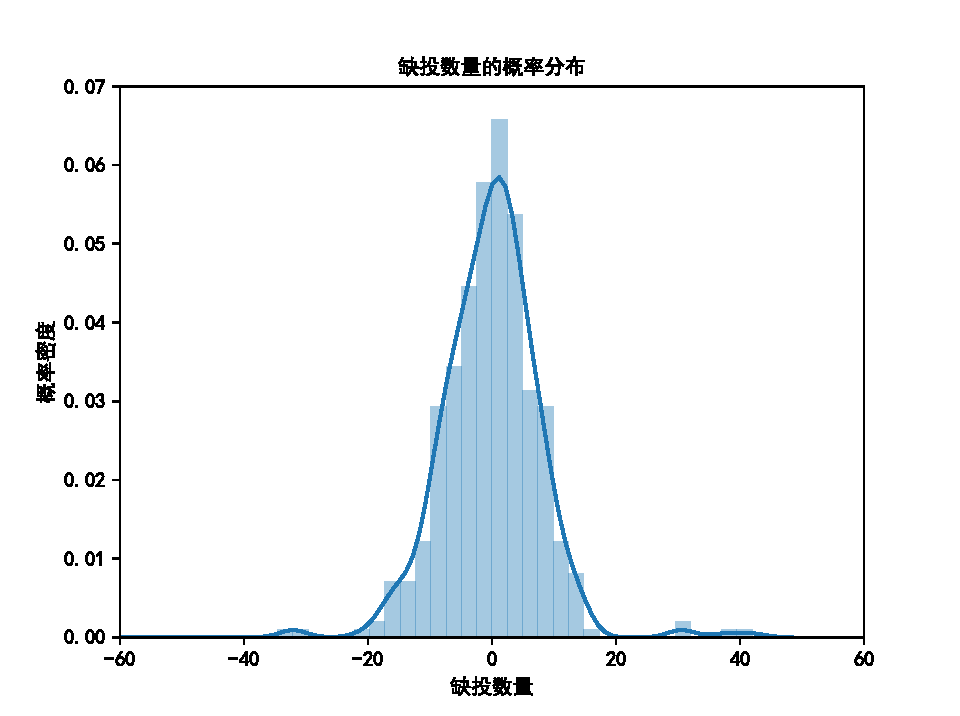
\includegraphics[width=\textwidth]{simulation.pdf}
	\caption{仿真实验中测试数据集的缺投情况统计。训练数据和测试数据各有50万次PV,同时有400个广告均有50的需求量。这个缺投量的分布和高斯分布非常相似。}
	\label{fig:delivery}
\end{figure}

\subsection{线上实验设置}

\subsection{关键指标}

\subsection{线上实验结果}

\begin{figure}[tb]
	\centering
	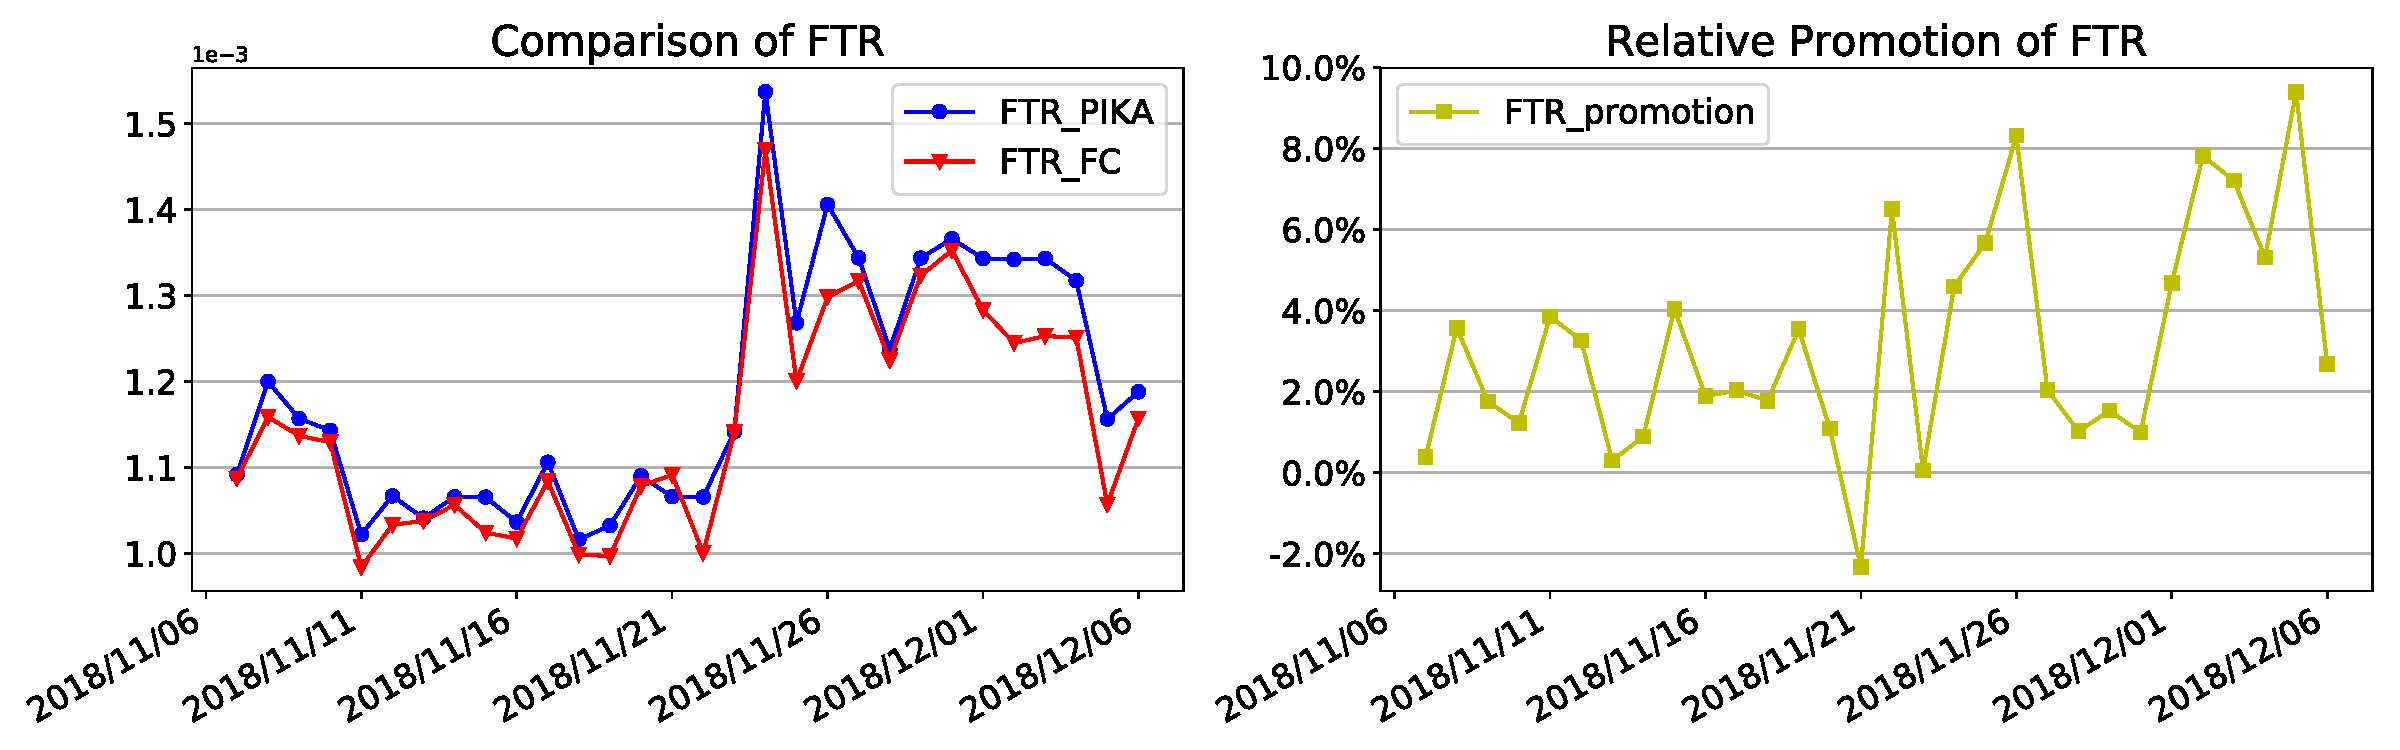
\includegraphics[width=\textwidth]{FTR.pdf}
	\caption{仿真实验中测试数据集的缺投情况统计。训练数据和测试数据各有50万次PV,同时有400个广告均有50的需求量。这个缺投量的分布和高斯分布非常相似。}
	\label{fig:delivery}
\end{figure}

\begin{figure}[tb]
	\centering
	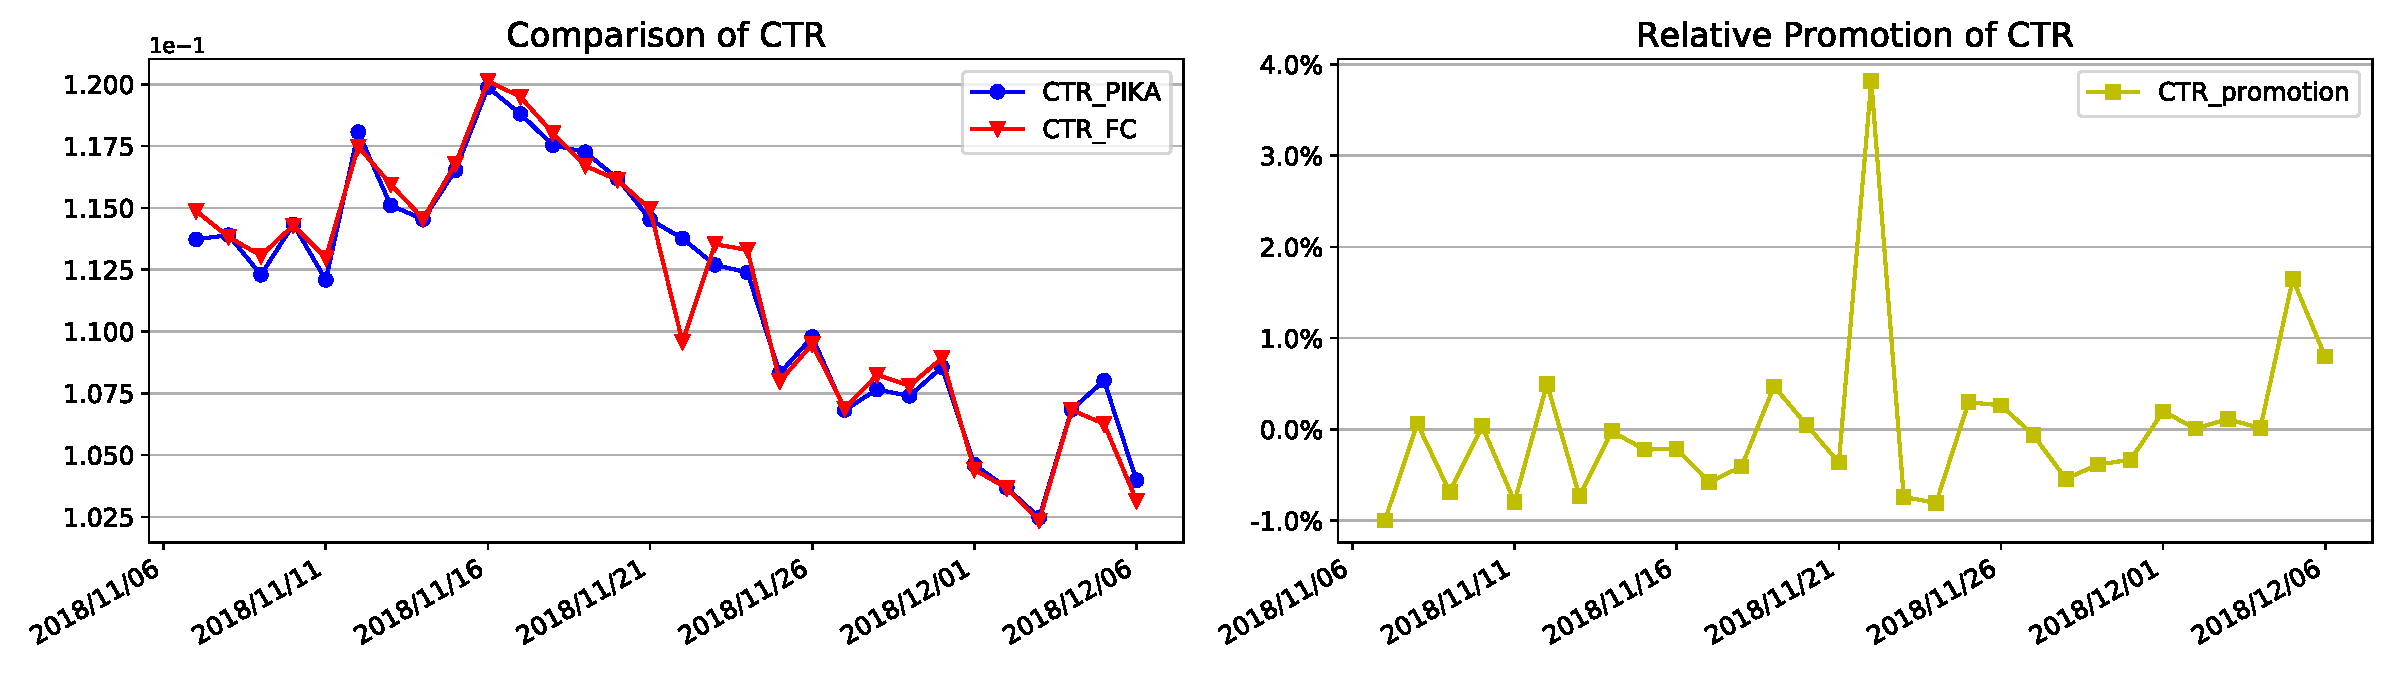
\includegraphics[width=\textwidth]{CTR.pdf}
	\caption{仿真实验中测试数据集的缺投情况统计。训练数据和测试数据各有50万次PV,同时有400个广告均有50的需求量。这个缺投量的分布和高斯分布非常相似。}
	\label{fig:delivery}
\end{figure}

\begin{figure}[tb]
	\centering
	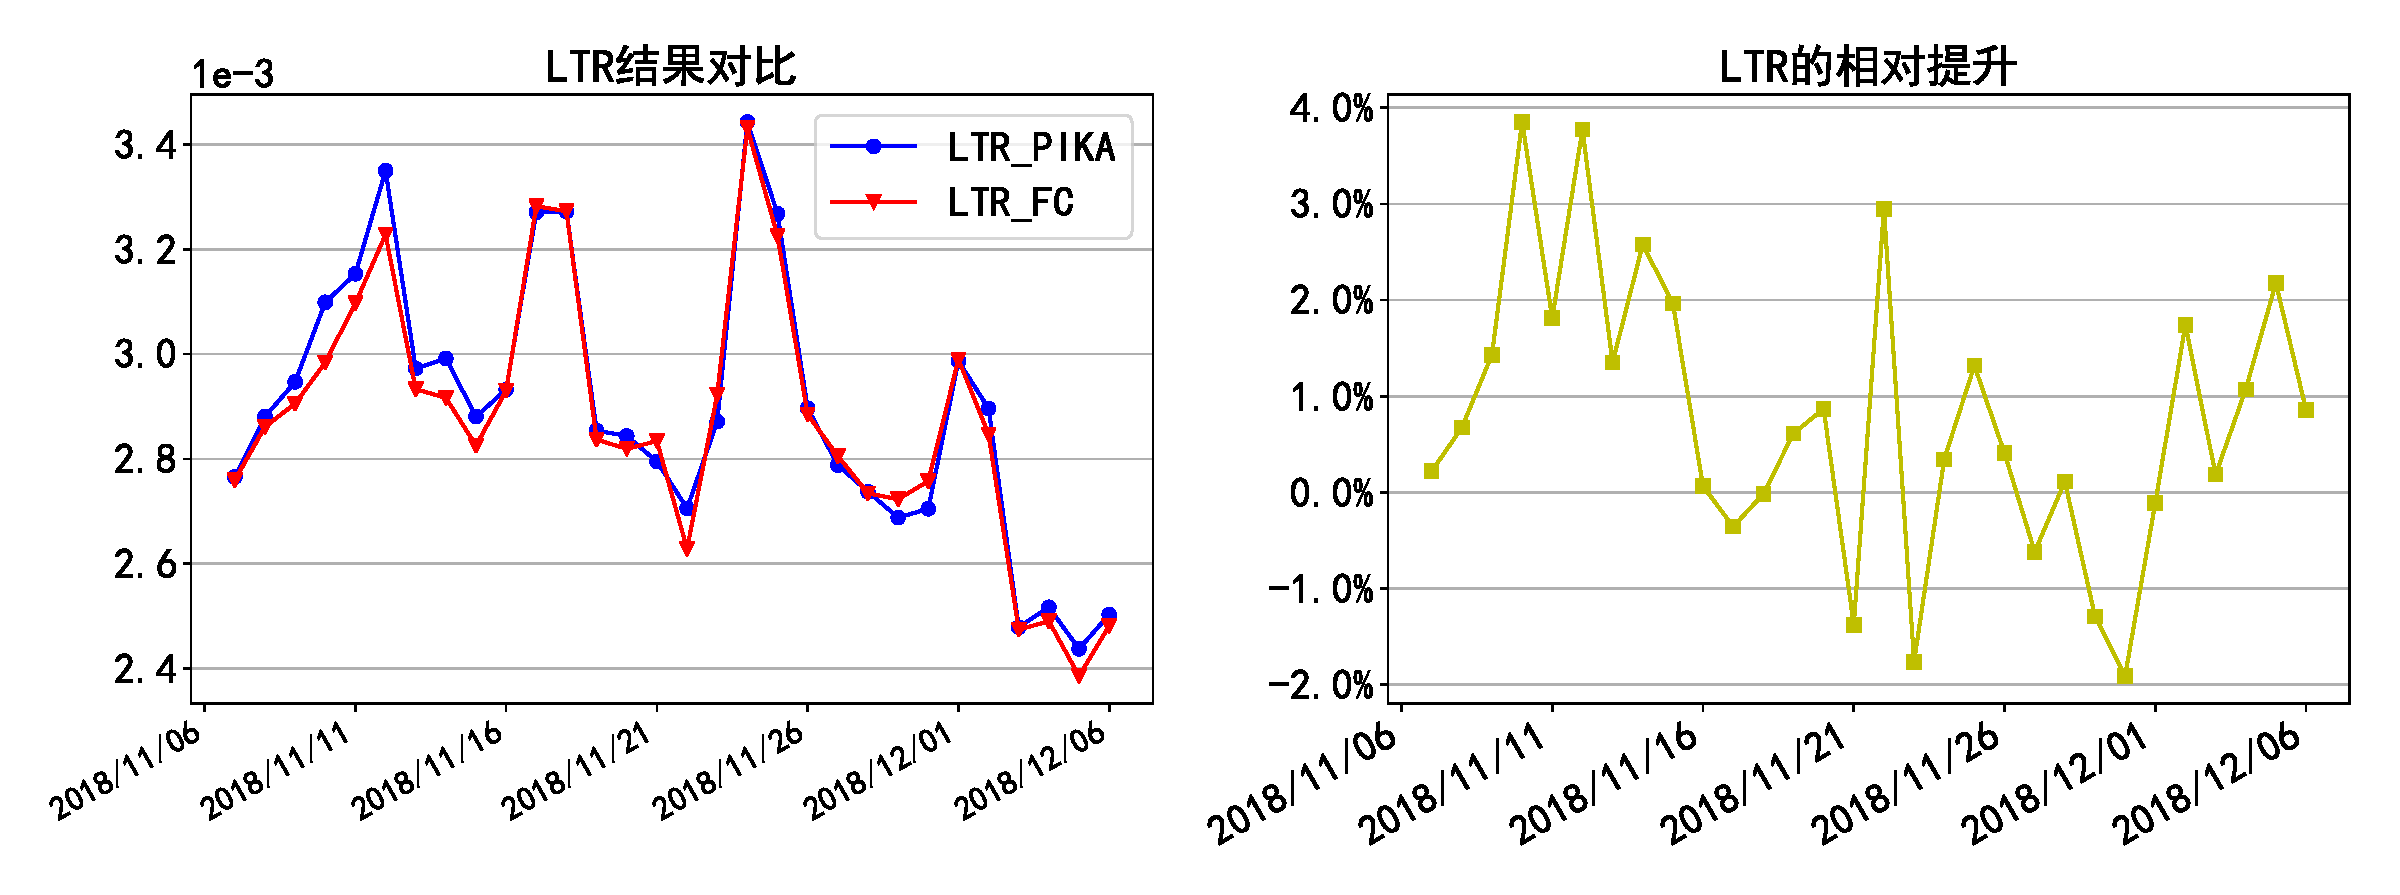
\includegraphics[width=\textwidth]{LTR.pdf}
	\caption{仿真实验中测试数据集的缺投情况统计。训练数据和测试数据各有50万次PV,同时有400个广告均有50的需求量。这个缺投量的分布和高斯分布非常相似。}
	\label{fig:delivery}
\end{figure}

\begin{figure}[tb]
	\centering
	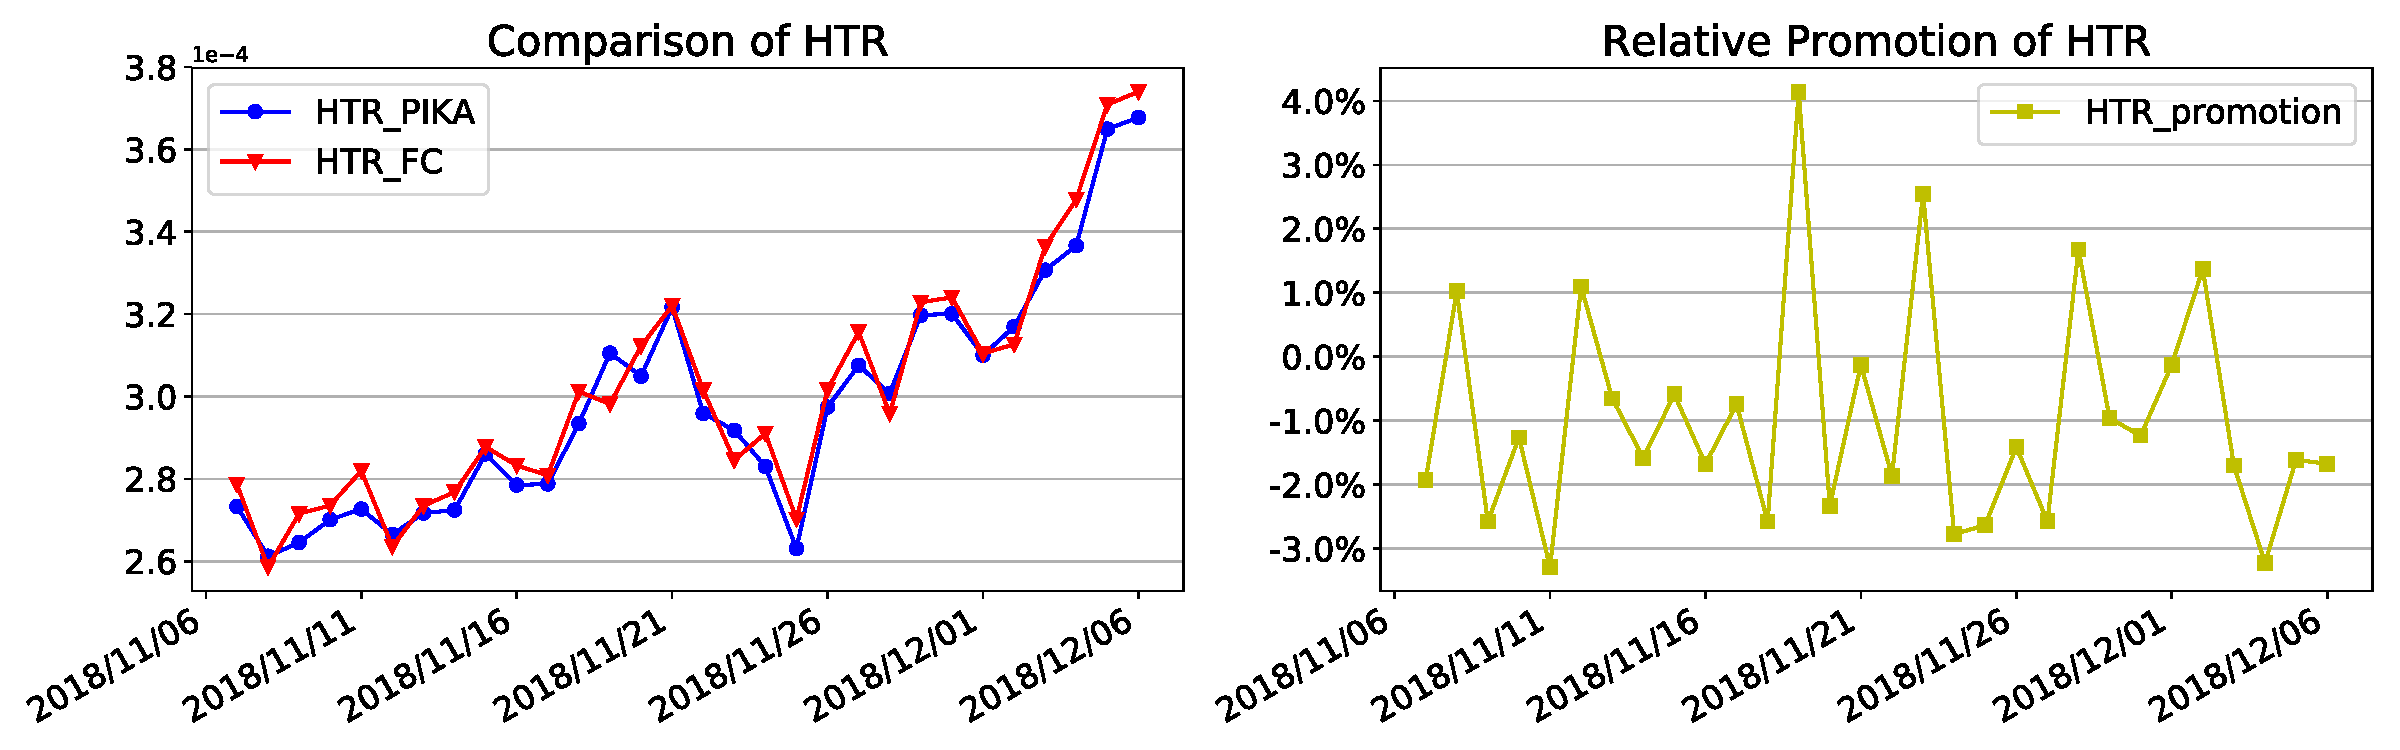
\includegraphics[width=\textwidth]{HTR.pdf}
	\caption{仿真实验中测试数据集的缺投情况统计。训练数据和测试数据各有50万次PV,同时有400个广告均有50的需求量。这个缺投量的分布和高斯分布非常相似。}
	\label{fig:delivery}
\end{figure}







\chapter{结论与展望}
\label{cha:conclusion}

\section{主要工作及贡献}

随着智能手机的普及和移动互联网的快速发展,定位问题及其后续应用吸引了越来越多的关注。虽然在相对空旷的室外场景下,GPS等基于卫星定位的定位方式已经能取得较高的定位精度,但是如何在遮挡严重的城市内以及室内定位目前还处在探索和发展阶段,而且如何解决GPS解决不了的发射源定位也是一个研究点。本文针对这两个发射源定位和接收端定位的问题,分别提出了几何模型发射源定位算法和基于曼哈顿切线距离的指纹定位算法,不仅只使用不需要额外硬件支持的接收信号强度作为特征,而且相比于经典算法提高了定位精度。同时,在获得用户位置后据此向用户推送广告是一种可行的商业模式,在保证广告主的广告曝光量的前提下最大化广告投放效果是一个有意义的研究方向。为此本文提出了一种保量推荐下的最优广告投放算法,既在性能和投放量方面满足要求,而且相比于之前部署的算法获得了广告投放效果的提升。具体研究成果和结论总结如下:
\begin{itemize}
	
	\item 我们提出了一个基于用户定位的广告投放服务系统,主要由定位和广告投放两大部分组成,之后我们详细介绍了整体系统架构,并着重说明了广告投放部分的系统架构。
	
	\item 针对用户作为信号发射源的定位问题,提出了基于接收信号强度的几何模型发射源定位算法,即提出一种新的优化目标函数,本质上是找到一个点使得它到所有圆的边缘的距离之和最小。同时,为了从理论上分析该方法的克拉美罗下界,我们提出了一种基于蒙特卡洛法的估计方法。为了确保我们的算法相比于经典的最大似然估计方法定位精度的提升具有统计意义,我们还推导了均方根误差的置信区间的计算方法。仿真结果表明在噪声较大的情况下,我们的算法能够取得更小的定位误差而且具有统计显著性,因为相比于无偏的最大似然估计,我们的算法在偏置和方差之间取得折中,即能更好的应对“过拟合”问题。最后我们也利用路测仪实地采集数据,实验结果表明我们的算法依然能取得更高的定位精度,说明我们的算法更适用于在真实环境中对发射源定位。
	
	\item 针对用户作为接收端且仅使用接收信号强度的定位问题,我们提出了基于曼哈顿切线距离的指纹定位算法。首先介绍了指纹定位中常用的K近邻算法以及常用的距离度量方式,并进一步分析了这些度量方式存在的问题,针对这些弊端提出了指数变换法和将切线距离应用于指纹定位中。在介绍切线距离及其背后的思想后,我们阐释了如何将切线距离应用于指纹定位中,并突破原来只有基于欧氏距离的切线距离的束缚,提出了基于曼哈顿距离的切线距离,以及在计算复杂度和定位精度之间折中的近似曼哈顿切线距离。我们在清华大学校园内三处不同信道特征的地方利用路测仪实地采集数据,并在数据集上开展实验。实验结果表明曼哈顿切线距离在所有三个数据集上均取得最小的定位误差,而近似曼哈顿切线距离则以小得多的计算复杂度取得了仅次于曼哈顿切线距离的定位精度。
	
	\item 针对保量推荐下的广告投放问题,我们提出了一种最优广告投放算法。在将实际问题抽象为数学优化问题后,利用凸优化方法中的KKT条件以及对偶问题推导出可以在线上高效投放广告的算法,同时还详细阐述了一些工程实现上的细节,以增加算法的实用性。在部署到线上之前,仿真实验证实了我们的算法的缺投量近似服从零均值正态分布,投放效果明显优于简单贪心算法。之后我们在中国最大的短视频平台之一——快手上开展了为期一个月的线上A/B测试,结果显示在计算时间和投放量等性能指标上我们的算法达标;在投放效果指标方面,我们的算法在最主要的指标上优于原先部署的算法而在其他次要指标上持平。最终得出结论:新算法在保证投放量的情况下可以获得比原先算法更好的投放效果。
\end{itemize}

\section{进一步工作展望}

虽然本论文的研究工作力求能够全面、深入的分析所涉及的问题,但是由于作者时间和能力的限制,仍有一些更深入、更本质的问题需要研究分析。
\begin{itemize}
	\item 在基于接收信号强度的几何模型发射源定位算法中,我们所提出的算法是一个非凸优化问题,这导致需要多次求解选取损失函数最小的一次,不仅时间开销大,而且还无法保证找到最优解。作为基线的最大似然估计也有同样的问题,不过已经有大量研究致力于将原问题转化为一个凸优化问题并力求减少由此带来的算法的解与真实最优解之间的差距。后续可以参考最大似然法的相关做法,应用于几何模型算法中,在定位误差少量增加的情况下减少计算时间。除此之外,在我们的算法中,路径损耗系数$\alpha$是需要提前设定好的参数,不能自适应的学习,从而会使得定位精度下降。如何自适应的学习$\alpha$也是一个可行的研究点。
	
	\item 在基于曼哈顿切线距离的指纹定位算法中,我们通过实测数据发现,在三个数据集上曼哈顿距离的定位精度均高于欧氏距离。首先需要确定这种现象是否具有普适性,如果答案是肯定的,则分析导致这种现象的原因将会具有重要意义。
	
	\item 在保量推荐下的最优广告投放算法中,我们的优化目标是投放广告的总分数最高,其中分数是关注率和点击率的线性组合。但是总最后的实验结果看来只有关注率提升了,点击率却几乎没有变化,而且一个月内几乎每天都是如此。为何唯独出现这种现象,而没有出现关注率不变、点击率提升或者二者皆提升的现象,是一个值得深入研究的点。
\end{itemize}






%%% 其它部分
\backmatter

%% 本科生要这几个索引,研究生不要。选择性留下。
% 插图索引
% \listoffigures
% 表格索引
% \listoftables
% 公式索引
% \listofequations


%% 参考文献
% 注意:至少需要引用一篇参考文献,否则下面两行可能引起编译错误。
% 如果不需要参考文献,请将下面两行删除或注释掉。
% 数字式引用
\bibliographystyle{thuthesis-numeric}
% 作者-年份式引用
% \bibliographystyle{thuthesis-author-year}
\bibliography{ref/refs}


%% 致谢
% 如果使用声明扫描页,将可选参数指定为扫描后的 PDF 文件名,例如:
% \begin{acknowledgement}[scan-statement.pdf]
\begin{acknowledgement}
  回首攻读硕士学位的三年时光,乃至在清华园度过的七年光阴,从起初对未来的迷茫疑惑,到后来认准方向并努力前行,最终现在可以从容的说出:一路走来,有憾无悔。这一路上,自己的努力很重要,但是际遇和帮助同样举足轻重。
  
  衷心感谢我的导师钟晓峰老师,他对我的谆谆教导帮助我在学术的道路上顺利前行,他宽容无私、温文尔雅的人格不仅使我在读研期间收获颇丰,也成为我学习的楷模。
  
  同时也非常感谢我在快手实习期间的领导李勇保先生,以及两位学长:程波波学长和于鑫学长。他们的专业水平与耐心教导使得我在快手的工作能够顺利完成,同时学有所成。
  
  此外,还要感谢实验室的陈皇卿师兄、金汝青师兄、龚贻华师兄和范晨晨师妹,以及张子卓同学和杨如达同学,他们在我犹豫困顿的时刻给予我鼓励和支持,也使我略显枯燥的科研生活变得不那么单调。
  
  感谢赵珵同学在我读研期间走进了我的生活之中,你的闪光点始终吸引着我,希望我们能够走到最后。
  
  最后,感谢我的父母在这二十多年来对我不求回报的付出和包容,儿子无以为报,唯有变成更好的自己让你们不用再为我操心。
\end{acknowledgement}


%% 附录
\begin{appendix}
\chapter{依期望采样的证明}
\label{cha:proof}

这里,我们将证明在允许一个广告被投放于同一PV两次的情况下,采样的期望等于计算所得的期望。

因为我们已经约束了$0 \le \bm{X}_{ij} \le 1$,因此划分操作可以很容易保证$\bm{p}$中的元素最多只被切分两次。于是现在只剩两种可能:
\begin{enumerate}[1)]
	\item $\bm{p}_j$没被切分。
	
	这种情况是平凡的,因为显然广告$j$被采样的期望就是$\bm{p}_j$。
	
	\item $\bm{p}_j$被切分。
	
	假设$\bm{p}_j$被分成两份:$p_1$和$p_2$。表\ref{tab:prob}展现了广告$j$被采样次数的概率,最后一行的期望是$p_1+p_2$,而这正好就是$\bm{p}_j$。
	\begin{table}[htb]
		\centering
		\caption{广告$j$被采样次数的概率(无限制)}
		\label{tab:prob}
		\begin{tabular}{cccc}
			\toprule
			被采样次数&0&1&2\\
			\midrule
			概率 & $ (1-p_1) (1-p_2)$ & $p_1 (1-p_2) +  (1-p_1)p_2$ & $p_1p_2$ \\
			\midrule
			期望 & \multicolumn{3}{c}{$p_1 (1-p_2) +  (1-p_1)p_2 + 2p_1p_2 = p_1 + p_2$} \\
			\bottomrule
		\end{tabular}
	\end{table}

\end{enumerate}

总之,如果一个广告可以被投放于同一个PV多于一次,则广告被采样,或者说被投放,的期望就是$\bm{p}$。

但是,如果广告$j$已经根据$p_1$被采样了,那么$p_2$就会被忽略的话,概率和期望就会变成表\ref{tab:prob_less}。此时被采样的期望不再等于$\bm{p}_j$,而是比$\bm{p}_j$少了$p_1p_2$。不过由于只有最多$m-1$个$\bm{p}_j$会被切分,这启发了我们最好切分那些$\bm{p}_j$较小的广告,从而减少采样的期望和计算所得期望的差距。

\begin{table}[htb]
	\centering
	\caption{广告$j$被采样次数的概率(最多被采样一次)}
	\label{tab:prob_less}
	\begin{tabular}{ccc}
		\toprule
		被采样次数&0&1\\
		\midrule
		概率 & $ (1-p_1) (1-p_2)$ & $p_1 +  (1-p_1)p_2$ \\
		\midrule
		期望 & \multicolumn{2}{c}{$p_1 + p_2 - p_1p_2$} \\
		\bottomrule
	\end{tabular}
\end{table}



\end{appendix}

%% 个人简历
\begin{resume}

  \resumeitem{个人简历}

  1993 年 11 月 20 日出生于辽宁省沈阳市。

  2012 年 9 月考入清华大学电子工程系电子信息科学类专业,2016 年 7 月本科毕业并获得工学学士学位。

  2016 年 9 月免试进入清华大学电子工程系攻读信息与通信工程学位至今。

  \researchitem{发表的学术论文} % 发表的和录用的合在一起

  % 1. 已经刊载的学术论文(本人是第一作者,或者导师为第一作者本人是第二作者)
  \begin{publications}
    \item Zhihe Li, Xiaofeng Zhong, and Zechen Cui. “Evaluating forecasting algorithm of realistic datasets based on machine learning.” Proceedings of the 2nd International Conference on Innovation in Artificial Intelligence. ACM, 2018. (EI 收录, 检索号:20183905853244.)
    \item Zhihe Li, Xiaofeng Zhong, and Jie Wei. “A Novel Geometry-Based Model for Localization Based on Received Signal Strength.” 2018 IEEE 87th Vehicular Technology Conference (VTC Spring). IEEE, 2018. (EI 收录, 检索号:20183205660551.)
    \item Zhihe Li, Xiaofeng Zhong, Jie Wei, and Han Shi. “The Application of Manhattan Tangent Distance in Outdoor Fingerprint Localization.” 2018 IEEE Global Communications Conference (GLOBECOM). IEEE, 2018. 
  \end{publications}

  % 2. 尚未刊载,但已经接到正式录用函的学术论文(本人为第一作者,或者
  %    导师为第一作者本人是第二作者)。
  % \begin{publications}[before=\publicationskip,after=\publicationskip]
    
  % \end{publications}

  % 3. 其他学术论文。可列出除上述两种情况以外的其他学术论文,但必须是
  %    已经刊载或者收到正式录用函的论文。
  \begin{publications}
    \item Huangqing Chen, Zhihe Li, Xiaofeng Zhong, and Jing Wang. "Energy-Saving Algorithm with Dimension Reduction on the Uplink for Multimedia Push." 2017 IEEE 86th Vehicular Technology Conference (VTC-Fall). IEEE, 2017. (EI 收录, 检索号:20181605013949 .)
  \end{publications}

  % \researchitem{研究成果} % 有就写,没有就删除
  % \begin{achievements}
    
  % \end{achievements}

\end{resume}


%% 本科生进行格式审查是需要下面这个表格,答辩可能不需要。选择性留下。
% 综合论文训练记录表
% 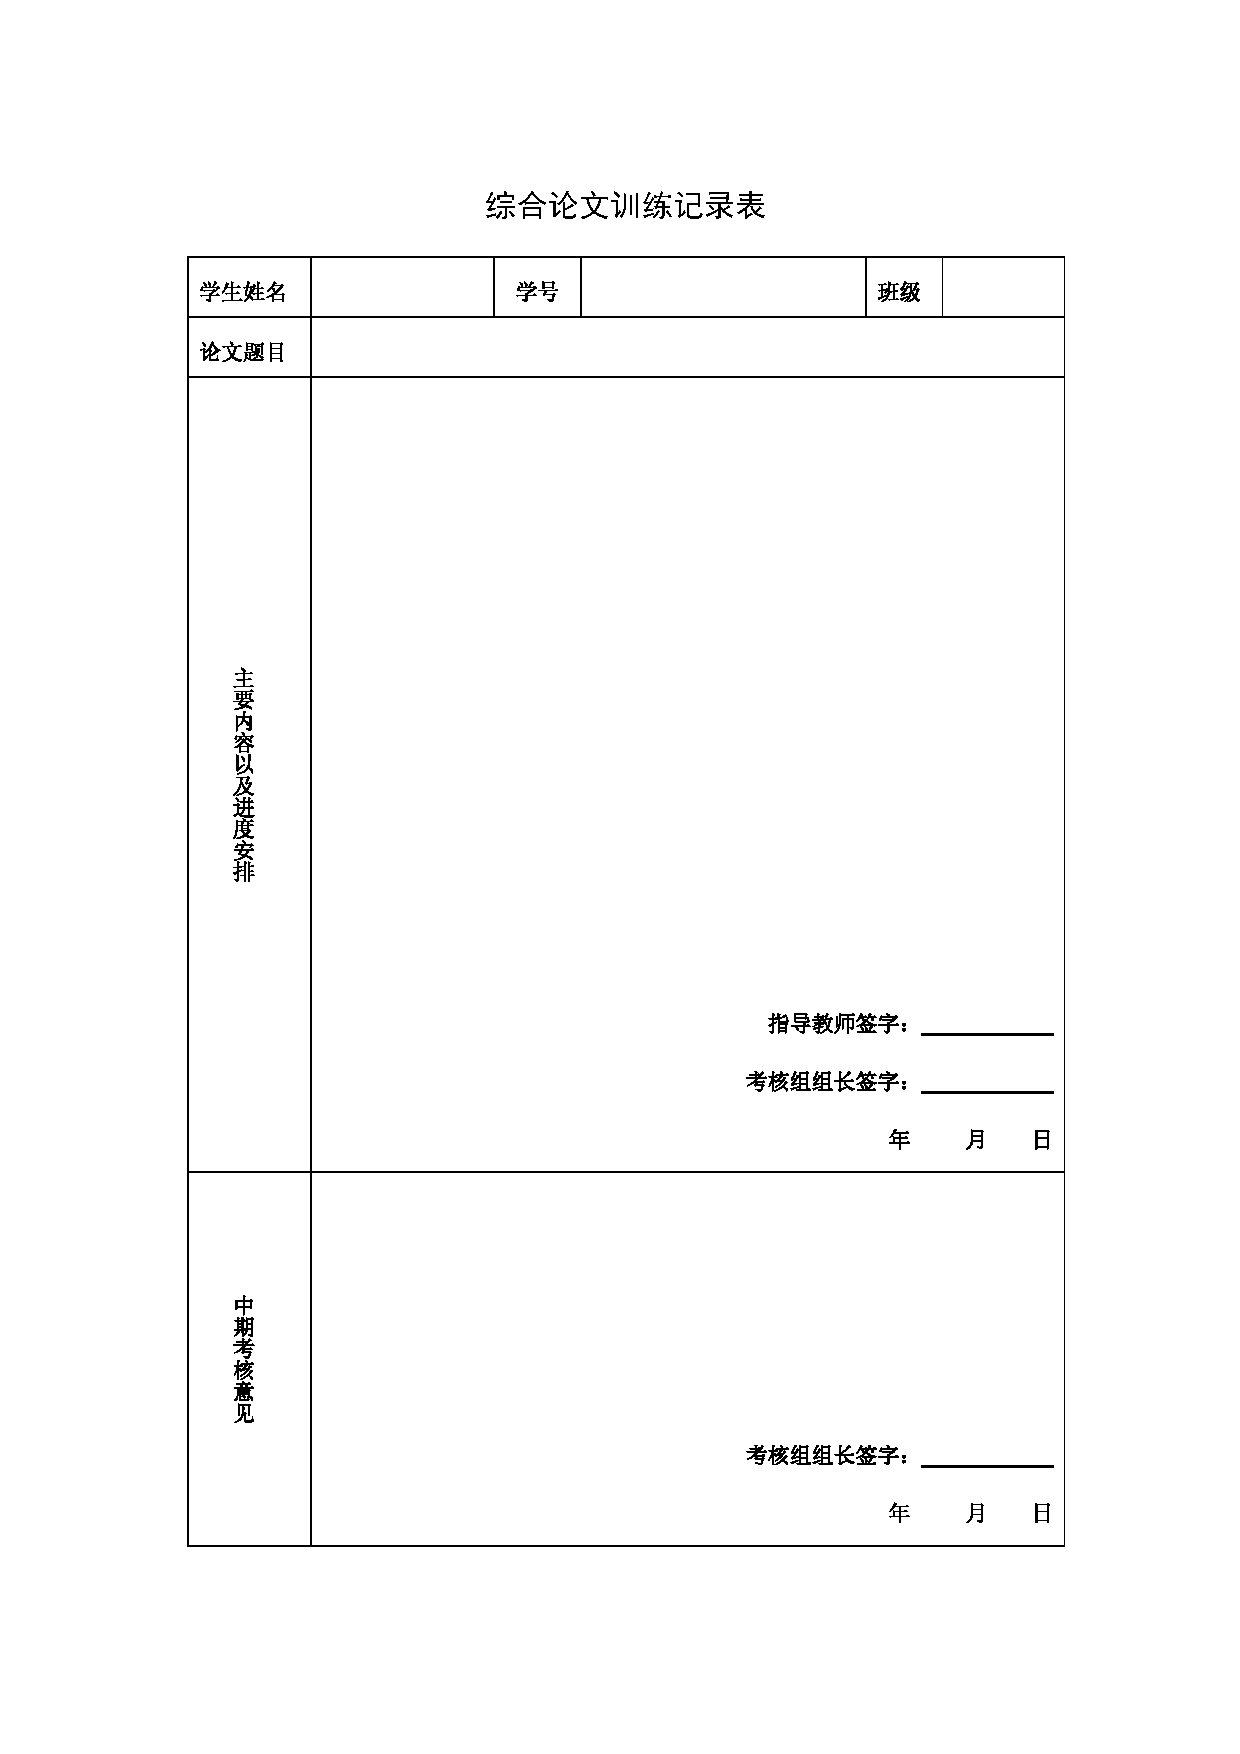
\includepdf[pages=-]{scan-record.pdf}
\end{document}
